%==============================================================================
% infufrgs-example.tex — Complete usage example for the infufrgs class
%
% This file is hereby placed in the public domain.
%
% CITAR: \cite{lamport1994latex}.
%
% Compile sequence:
%   pdflatex infufrgs-example
%   bibtex   infufrgs-example
%   pdflatex infufrgs-example
%   pdflatex infufrgs-example
%==============================================================================

% Select program (ppgc, pgmicro, cic, ecp, ppgl) and document type
% (diss/mestrado, tese/doutorado, tc/dipl, ti, rp, espec, pep, prop-tese,
%  plano-doutorado).  Add `english' for English-language documents.
\documentclass[cic,tc]{infufrgs}

% If using pdfLaTeX, declare the input encoding (UTF-8 is recommended).
% Not needed with XeLaTeX or LuaLaTeX.
\usepackage[utf8]{inputenc}

% For figure inclusion
\usepackage{graphicx}

% For professional-looking tables
\usepackage{booktabs}
\usepackage{colortbl}
\usepackage{multirow}
\usepackage{float}

% Optionally load math packages
\usepackage{amsmath}
\usepackage{tikz}
\usepackage{subcaption}
\usetikzlibrary{shapes.geometric, arrows.meta, positioning, angles, quotes, calc, babel}

% Evita o estiramento vertical de espacos (flushbottom) entre figuras [H] e texto
\raggedbottom
\allowdisplaybreaks

\DeclareMathOperator{\bd}{bd}
\DeclareMathOperator{\rpos}{rpos}

%------------------------------------------------------------------------------
% Document metadata
%------------------------------------------------------------------------------
\title{Otimização Inteira Mista Aplicada à Geração de Mapas Esquemáticos de Redes de Transporte: Um Estudo de Caso sobre o Sistema de Ônibus de Porto Alegre}
\translatedtitle{Mixed Integer Optimization Applied to the Generation of Schematic Maps of Transport Networks: A Case Study on the Bus System of Porto Alegre}

% Author: \author{Surname}{First Name(s)}
\author{Spellmeier Neves}{Gustavo}
% Multiple authors are supported:
%\author{Flaumann}{Frida Gutenberg}

% Advisor (title is optional): \advisor[Title]{Surname}{First Name(s)}
\advisor[Prof.~Dr.]{Mello Schnorr}{Lucas}
% Co-advisor is optional:
%\coadvisor[Prof.~Dr.]{Knuth}{Donald Ervin}

% Date of the defence.  Defaults to the current month and year if omitted.
%\date{maio}{2001}

% Location of the defence.  Defaults to Porto Alegre, RS.
%\location{Itaquaquecetuba}{SP}

%------------------------------------------------------------------------------
% Keywords — use Title Case; up to 10 keywords per language
%------------------------------------------------------------------------------
\keyword{Mapas Esquemáticos}
\keyword{Programação Inteira Mista}
\keyword{Transporte Público}
\keyword{Otimização Combinatória}
\keyword{Desenho de Grafos}
\keyword{GTFS}

\translatedkeyword{Schematic Maps}
\translatedkeyword{Mixed-Integer Programming}
\translatedkeyword{Public Transport}
\translatedkeyword{Combinatorial Optimization}
\translatedkeyword{Graph Drawing}
\translatedkeyword{GTFS}

%------------------------------------------------------------------------------
% Nominata — override individual fields if the bundled defaults are stale.
% Example:
%   \renewcommand{\nominataReit}{Prof\textsuperscript{a}.~Nome Sobrenome}
%   \renewcommand{\nominataReitname}{Reitora}
%------------------------------------------------------------------------------

%==============================================================================
\begin{document}
%==============================================================================

% Title page + CIP (or nominata page)
\maketitle

%------------------------------------------------------------------------------
% Optional front matter
%------------------------------------------------------------------------------
\begin{dedicatoria}
  \begin{minipage}{0.7\textwidth}
    \textit{``Cada um exerça o dom que recebeu para servir aos outros, administrando fielmente a graça de Deus nas suas múltiplas formas.''}
    \par\vspace{0.3cm}\hfill --- 1 Pedro 4:10
  \end{minipage}
\end{dedicatoria}

\begin{agradecimentos}
    Primeiramente, à minha mãe, Roseli Spellmeier Neves, e ao meu pai, Paulo Ricardo Neves, por terem me proporcionado todas as oportunidades de estudo e por terem acreditado no meu potencial antes de qualquer pessoa; pelo apoio incondicional e pelo lar acolhedor que sempre me ofereceram. Sem vocês, eu definitivamente não estaria onde me encontro hoje.
    
    À minha noiva, Katiely Scharnesky, por todos os momentos maravilhosos que compartilhamos, especialmente neste último ano; por me incentivar a me tornar uma pessoa melhor, e pelo carinho e amor constantes, mesmo nos períodos mais difíceis.

    Aos meus amigos próximos de Canoas e de Porto Alegre por todos os momentos divertidos, pelas conversas e pela companhia tão agradável, trazendo leveza e descontração em momentos complicados. Em especial, aos meus amigos Marco Antônio Chitolina e Gabriel Cortezi por terem me acolhido em suas casas durante o período das enchentes de 2024.

    Aos meus amigos da igreja e do meu grupo de crescimento por estarem ao meu lado na minha caminhada de fé, especialmente no meu período de retorno após as enchentes.

    À Universidade Federal do Rio Grande do Sul (UFRGS) e ao Instituto de Informática (INF) pela oportunidade de vivenciar um ensino superior de excelência. Ao meu orientador, Prof.~Dr.~Lucas Mello Schnorr, por ter proposto o tema deste trabalho, o qual tive grande satisfação em desenvolver, e pelo apoio e orientação ao longo de toda a sua realização.

    Por fim, agradeço a Deus por ter me sustentado durante toda a minha jornada, pelo milagre da vida e pelas lições que vão além da compreensão humana. A Ele seja dada toda a glória, agora e para sempre.

\end{agradecimentos}

%------------------------------------------------------------------------------
% Abstract in the primary language
%------------------------------------------------------------------------------
\begin{abstract}
  Este trabalho apresenta o desenvolvimento e a implementação de um modelo de Programação Linear Inteira Mista (MIP) para a geração automatizada de mapas esquemáticos de transporte público, utilizando como base a rede de ônibus de Porto Alegre. A metodologia fundamenta-se no algoritmo de Nöllenburg e Wolff, focando na conversão de grafos geográficos complexos em diagramas que priorizam a legibilidade e a preservação do mapa mental do usuário. Somado à metodologia há o estudo necessário sobre o caso específico de Porto Alegre, proveniente do grande número de linhas e paradas de ônibus, a fim de simplificar ou abstrair o problema. O modelo incorpora restrições rígidas de topologia e geometria, além de funções objetivo voltadas à minimização de curvas e otimização do espaçamento entre estações. O trabalho busca demonstrar a viabilidade do uso de solvers de alto desempenho para simplificar visualmente redes de larga escala, transformando dados brutos do padrão GTFS em ferramentas de auxílio à visualização de movimentação urbana mais eficientes.
\end{abstract}

%------------------------------------------------------------------------------
% Abstract in the second language (translatedabstract)
%------------------------------------------------------------------------------
\begin{translatedabstract}
  This work presents the development and the implementation of a Mixed Integer Programming (MIP) model for the automated generation of schematic public transport maps, using as a base the bus network of Porto Alegre. The methodology is founded on the algorithm of Nöllenburg and Wolff, focusing on the conversion of complex geographic graphs into diagrams that prioritize readability and the preservation of the user's mental map. Added to the methodology is the necessary study on the specific case of Porto Alegre, stemming from the large number of bus lines and stops, in order to simplify or abstract the problem. The model incorporates rigid constraints of topology and geometry, in addition to objective functions aimed at the minimization of bends and optimization of the spacing between stations. The work seeks to demonstrate the feasibility of the use of high-performance solvers to visually simplify large-scale networks, transforming raw data of the GTFS standard into more efficient auxiliary tools for the visualization of urban movement.
\end{translatedabstract}

%------------------------------------------------------------------------------
% Lists
%------------------------------------------------------------------------------
\tableofcontents

\listoffigures

\listoftables

% Optional: list of abbreviations
\begin{listofabbrv}{UFRGS}
  \item[ABNT] Associação Brasileira de Normas Técnicas
  \item[INF]  Instituto de Informática
  \item[MIP] Programação Inteira Mista
  \item[GTFS] Especificação Geral de Feeds de Transporte Público
  \item[EPTC] Empresa Pública de Transporte e Circulação
  \item[CPTM] Companhia Paulista de Trens Metropolitanos
  \item[UFRGS] Universidade Federal do Rio Grande do Sul
  \item[GUI] Interface Gráfica do Usuário
\end{listofabbrv}

% Optional: list of symbols
% \begin{listofsymbols}{$\alpha$}
%   \item[$\alpha$] Alpha coefficient
% \end{listofsymbols}

%==============================================================================
% Text body
%============================================================================== 

\chapter{Introdução}

As redes de transporte público são parte integral do cotidiano de grande parte da população. No Brasil, um país com forte aderência ao transporte rodoviário, o transporte por ônibus assume um papel de ainda maior destaque. Embora existam ferramentas digitais que auxiliam na locomoção urbana, como os aplicativos Moovit, Cittamobi e Google Maps, que planejam rotas e indicam as linhas a serem utilizadas, nota-se a ausência de uma visão geral e esquematizada das rotas de ônibus de Porto Alegre. Essa lacuna é especialmente sentida na ausência de mapas que possam ser consultados de forma independente, sem a necessidade de conexão à internet ou de dispositivos eletrônicos.

Em metrópoles como Porto Alegre, a visualização da rede de transporte torna-se uma tarefa desafiadora devido à alta complexidade e sobreposição das linhas. Mapas puramente geográficos perdem sua eficácia, gerando representações confusas que dificultam a compreensão dos trajetos. Para contornar esse problema, muitas cidades adotam mapas esquemáticos, que abstraem a geografia para priorizar a legibilidade e a usabilidade. No entanto, a elaboração manual desses mapas é um processo de alto custo e que demanda tempo, um obstáculo significativo para sistemas de transporte que, como o de Porto Alegre, estão em constante mudança e possuem uma complexidade expressiva, englobando aproximadamente 300 linhas em operação e quase quatro mil pontos de parada espalhados por uma malha viária densa e ramificada.

A geração automática de mapas surge como uma abordagem promissora para superar tais desafios. Nesse campo, destaca-se o trabalho de Nöllenburg e Wolff \cite{Nollenburg}, que propõem um modelo de Programação Inteira Mista (MIP) para a esquematização de redes de metrô. O modelo emprega restrições rígidas (\textit{hard constraints}) para garantir a correção topológica e geométrica, e restrições flexíveis (\textit{soft constraints}) para otimizar a qualidade estética do mapa, minimizando, por exemplo, o número de curvas e padronizando o comprimento das arestas. A aplicação bem-sucedida do algoritmo em redes como as de Sydney e Londres demonstra seu potencial para gerar layouts de alta qualidade sem a necessidade de intervenção humana. Ademais, o uso de um modelo matemático mostra-se ainda mais vantajoso para redes de ônibus do que para metrôs, pois além de rotas de ônibus sofrerem alterações operacionais com frequência muito maior do que linhas férreas, a formulação matemática permite fixar facilmente parte de uma solução anterior, possibilitando a atualização incremental do mapa sem alterá-lo por completo.

No entanto, a aplicação direta desses modelos de esquematização ao sistema de ônibus de Porto Alegre esbarra em dois grandes obstáculos. O primeiro é a \textbf{inexistência de uma representação em grafo formal e estruturada da rede}. Os dados públicos disponíveis nos feeds GTFS~\cite{gtfs_spec} da Empresa Pública de Transporte e Circulação (EPTC)~\cite{EPTCGTFS} registram itinerários operacionais e coordenadas geográficas brutas, mas não fornecem uma topologia unificada de rede conectada, com relações claras de adjacência, fusão de paradas adjacentes e modelagem de corredores compartilhados. O segundo obstáculo reside na \textbf{escala e complexidade computacional}: enquanto os estudos clássicos focam em redes de metrô com poucas dezenas ou centenas de estações (como a de Londres, com cerca de 300 nós), a malha de ônibus de Porto Alegre engloba quase 400 linhas e cerca de quatro mil paradas físicas (totalizando 3.831 nós e 4.382 arestas na malha de conexões), com trajetos de geometrias sinuosas e bifurcações não triviais. Em decorrência dessas diferenças, a aplicação direta e sem modificações do modelo de Nöllenburg e Wolff à rede de Porto Alegre não produziu resultados satisfatórios em testes preliminares, consequência da complexidade computacional proibitiva que impede a obtenção de soluções pelos solvers em tempo hábil.

Diante dessa inviabilidade prática, este trabalho investiga a viabilidade de modelar, simplificar e esquematizar automaticamente a malha de transporte por ônibus de Porto Alegre via MIP, dividindo o problema entre a estruturação dos dados e a formulação da otimização. Como principais contribuições, destacam-se: (1)~a modelagem de um grafo híbrido integrando os dados operacionais de paradas e o traçado físico das vias a partir do padrão GTFS; (2)~um pipeline de abstração e simplificação topológica capaz de contrair a escala da rede e eliminar nós de grau crítico; (3)~a adaptação e implementação de formulações MIP em Julia/CPLEX voltadas às particularidades do transporte rodoviário urbano; (4)~uma estratégia iterativa de para correção de distorções geométricas relativas sem a imposição de restrições rígidas de não-cruzamento; e (5)~a validação empírica quantitativa e qualitativa do método utilizando a malha das bacias operacionais de Porto Alegre.

O restante deste trabalho está estruturado da seguinte forma. O Capítulo~\ref{cap:trabalhos_relacionados} revisita o estado da arte na geração automatizada de mapas esquemáticos, contemplando a linhagem de otimização inteira mista, extensões de layout, abordagens voltadas a redes de ônibus e estudos de percepção do usuário. O Capítulo~\ref{cap:fundamentacao} estabelece a fundamentação teórica em cartografia esquemática e teoria dos grafos, detalhando a formulação matemática clássica de Nöllenburg e Wolff. O Capítulo~\ref{cap:metodologia} descreve a metodologia e o desenvolvimento do sistema, abrangendo a arquitetura em Julia, a construção do Grafo a partir de dados GTFS, as heurísticas de abstração topológica, as formulações MIP adaptadas, e o mecanismo iterativo de correção geométrica. O Capítulo~\ref{cap:resultados} discute os resultados experimentais obtidos nos recortes operacionais de Porto Alegre, analisando quantitativa e qualitativamente a convergência, tempos de execução, ocorrência de cruzamentos e legibilidade dos diagramas gerados. Por fim, o Capítulo~\ref{cap:conclusao} expõe as conclusões do trabalho, sintetizando suas contribuições, limitações de escalabilidade e perspectivas para pesquisas futuras.

\chapter{Trabalhos Relacionados}
\label{cap:trabalhos_relacionados}

A geração automática de mapas esquemáticos de transporte é um problema que se encontra na interseção da otimização combinatória, da cartografia computacional e da visualização de informação. O panorama atual da literatura pode ser organizado em torno de quatro eixos principais: (i) a linhagem de otimização inteira mista fundada por Nöllenburg e Wolff, que constitui a base metodológica direta deste trabalho; (ii) os refinamentos de layout, estilo e subtarefas como rotulagem, que estendem o paradigma original; (iii) os poucos trabalhos especificamente voltados a redes de ônibus e mapas de rota; e (iv) os estudos de usabilidade e percepção do usuário, que situam os critérios de qualidade no contexto do uso real.

\section{Linhagem MIP e Otimização Exata}

O trabalho seminal de Nöllenburg e Wolff \cite{Nollenburg}, descrito em detalhe na Seção~\ref{cap:fundamentacao}, estabelece o paradigma central adotado neste TCC. A formulação MIP modela as propriedades desejáveis de um mapa esquemático como restrições lineares e as integra a uma função objetivo que penaliza curvas, desvios de posição relativa e comprimento excessivo de arestas. Testada nas redes de transporte sobre trilhos de Sydney e Londres — redes com dezenas a poucas centenas de estações e topologia regular —, a formulação mostrou-se capaz de gerar layouts de alta qualidade de forma totalmente automatizada. A Figura~\ref{fig:comparativo_sydney} ilustra a eficácia desse método comparando o mapa esquemático oficial da rede de trens de Sydney (Figura~\ref{fig:sydney_original}) com o layout automatizado obtido pela formulação de Nöllenburg e Wolff (Figura~\ref{fig:sydney_nollenburg}); cabe notar que eventuais diferenças de linhas e estações entre ambos decorrem da defasagem temporal entre a publicação do artigo de Nöllenburg e Wolff (2015) e a versão atual do mapa oficial utilizada para ilustração. Tais redes metropolitanas de trilhos, contudo, diferem substancialmente da malha de ônibus de Porto Alegre tanto em escala quanto em irregularidade geométrica, o que motiva as adaptações propostas neste trabalho.

\begin{figure}[H]
    \centering
    \begin{subfigure}[b]{0.48\textwidth}
        \centering
        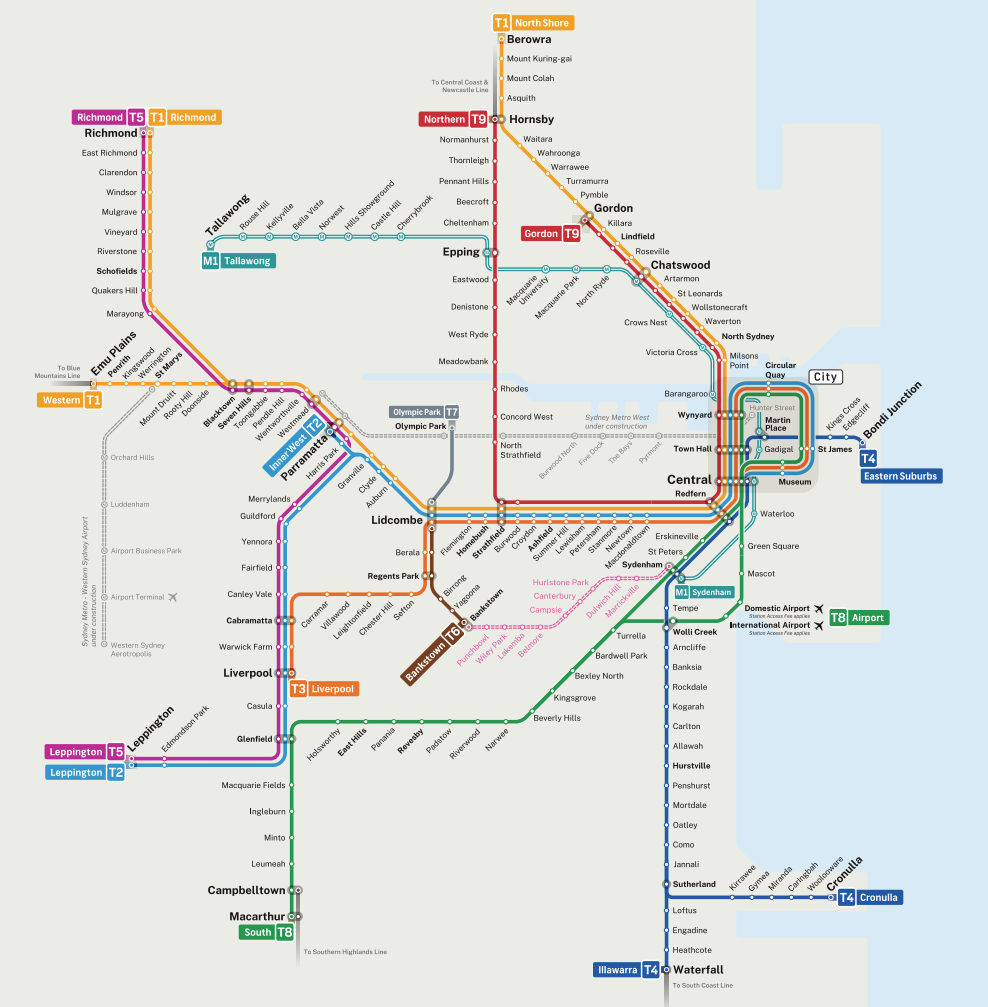
\includegraphics[width=\linewidth]{imagens/sydney_original.png}
        \caption{Mapa esquemático oficial da rede de trens de Sydney.}
        \label{fig:sydney_original}
    \end{subfigure}
    \hfill
    \begin{subfigure}[b]{0.48\textwidth}
        \centering
        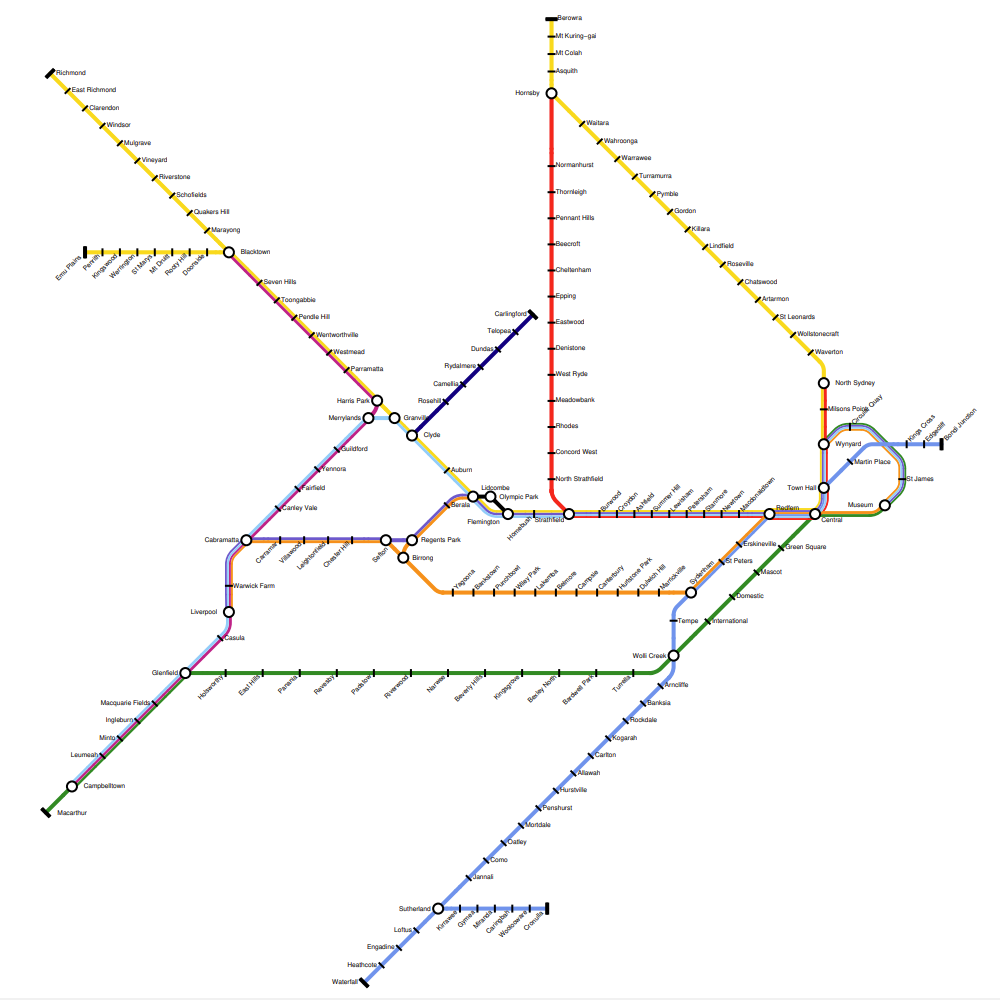
\includegraphics[width=\linewidth]{imagens/sydney_nollenburg.png}
        \caption{Layout gerado via MIP por Nöllenburg e Wolff.}
        \label{fig:sydney_nollenburg}
    \end{subfigure}
    \caption{Comparativo da rede de Sydney: mapa oficial de referência e resultado da esquematização por programação inteira mista.}
    \label{fig:comparativo_sydney}
    \vspace{0.15cm}
    \par\raggedright\footnotesize\textit{Fonte: Adaptado de Transport for NSW~\cite{TransportNSW2026} e Nöllenburg e Wolff~\cite{Nollenburg}.}
\end{figure}

Oke e Siddiqui \cite{Oke} identificam o custo computacional elevado como o principal gargalo do modelo original e propõem duas simplificações estruturais para contorná-lo. A primeira consiste em relaxar as variáveis de coordenada de inteiras para contínuas, reduzindo o espaço de busca do solver sem comprometer a octilinearidade da solução, visto que esta é garantida pelas restrições de direção. A segunda elimina a penalidade de comprimento de arestas da função objetivo, convertendo-a em uma restrição rígida de comprimento máximo; o modelo passa, assim, a ser biobjetivo, otimizando apenas curvas e preservação de posição relativa. Os autores também propõem o método AUGMECON2~\cite{MAVROTAS20139652} como alternativa à combinação linear de pesos, permitindo explorar automaticamente o conjunto de soluções Pareto-ótimas em uma única execução. Este trabalho aplica as simplificações de Oke e Siddiqui e avalia a compatibilidade do AUGMECON2 com o ciclo iterativo de correção de distorções geométricas proposto (Seção~\ref{subsec:correcao_distorcoes}).

Lan et al. \cite{TianLan} deslocam o foco do nível local para o nível global da rede, argumentando, com base em estudos de psicologia cognitiva, que a percepção visual humana opera de forma hierárquica do ``global para o local''. O trabalho é especialmente relevante para justificar decisões de abstração em redes grandes e densas como a de Porto Alegre, nas quais a fidelidade local deve ceder espaço à clareza global. Já van Dijk e Terziadis \cite{ThomasC} adotam uma perspectiva distinta ao proporem um sistema de iteração rápida assistida por algoritmo, em que o designer humano guia o processo em vez de uma otimização totalmente automatizada, o que delimitaria assim o espaço em que a abordagem deste TCC atua com maior autonomia.

\section{Trabalhos sobre Mapas de Ônibus e Outros Modelos}

A grande maioria dos trabalhos sobre mapas esquemáticos automáticos tem como objeto redes de metrô ou ferroviárias. Entre as raras iniciativas voltadas especificamente ao transporte rodoviário coletivo, o trabalho de Sadahiro et al. \cite{Sadahiro2016} figura como o estudo mais relevante e aprofundado na literatura acerca do design computacional de mapas para rotas de ônibus. Os autores realizam um levantamento sistemático das dificuldades inerentes a esse modal e identificam seis anomalias visuais críticas, decompostas em duas etapas metodológicas: na fase de ordenação de linhas, busca-se mitigar espaços vazios desnecessários entre rotas, desvios laterais ao longo de retas contínuas e cruzamentos acidentais; na fase de traçado geométrico, tratam-se os desalinhamentos das linhas com a pista viária, as sobreposições entre rotas em vias muito próximas e as curvas excessivamente fechadas em esquinas. Para solucionar a alocação combinatória das linhas nas faixas viárias, os autores recorrem a meta-heurísticas de busca tabu, combinadas a translações geométricas e a um esforço considerável de edição manual final em ambiente de Sistema de Informações Geográficas (SIG).

Embora de grande valor metodológico, a proposta de Sadahiro et al. parte de uma premissa cartográfica fundamentalmente distinta da adotada neste TCC: enquanto os autores buscam a melhor representação viária possível em escala geográfica estrita 1:1 — mantendo as rotas sobrepostas ao mapa viário real e promovendo apenas translações locais de faixas —, o objetivo deste trabalho é justamente modificar, abstrair e retificar as geometrias da rede. Ao distanciar-se da fidelidade geográfica microscópica para adotar um layout esquemático octilinear gerado de forma autônoma via Programação Inteira Mista (MIP), este trabalho prioriza a desobstrução visual, a uniformidade de trajetos e a redução da carga cognitiva na identificação dos fluxos de transporte da malha.

Em contrapartida às abordagens exatas, Galvão \cite{Galvao2016} e Galvão et al. \cite{Galvao2017} exploram algoritmos genéticos para a esquematização octilinear de linhas de ônibus; embora produzam diagramas simplificados e apresentem execução mais rápida, tais métodos heurísticos não fornecem garantias formais de otimalidade nem a estrita preservação topológica assegurada pelos modelos MIP. No campo das formulações inteiras, Xu et al. \cite{Yingying} propõem uma variação do modelo MIP que gera layouts em círculos concêntricos em vez da grade octilinear, demonstrando a versatilidade do paradigma de otimização exata para diferentes objetivos estéticos. A Figura~\ref{fig:concentric_map} exemplifica essa abordagem aplicada à malha de metrô de Pequim, organizando os anéis perimetrais e eixos radiais da rede sobre anéis concêntricos.

\begin{figure}[H]
    \centering
    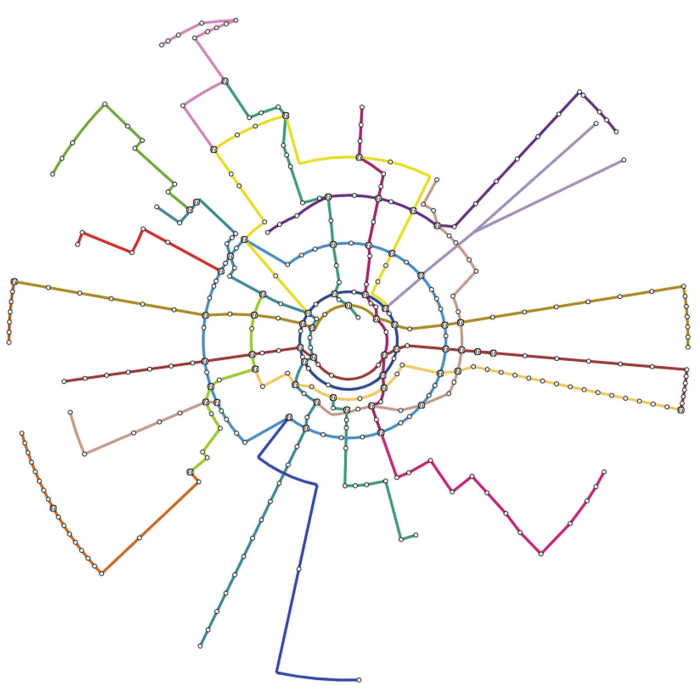
\includegraphics[width=0.62\textwidth]{imagens/conncentric_map.png}
    \caption{Layout esquemático concêntrico da rede de metrô de Pequim gerado via otimização inteira mista.}
    \label{fig:concentric_map}
    \vspace{0.15cm}
    \par\raggedright\footnotesize\textit{Fonte: Xu et al.~\cite{Yingying}.}
\end{figure}

Em uma perspectiva voltada à escalabilidade global, Brosi e Bast \cite{brosi2023large} investigam a geração automatizada de mapas de transporte para todo o planeta a partir de dados abertos do OpenStreetMap. O pipeline proposto pelos autores extrai geometrias viárias via consultas, sintetiza um grafo topológico desprovido de sobreposições por meio de amostragem e fusão incremental de vias, e ordena as linhas nos segmentos minimizando cruzamentos em nós. Contudo, ao abordarem a esquematização dos traçados, os autores relatam que a aplicação de modelos exatos de Programação Linear Inteira (ILP) torna-se computacionalmente proibitiva para redes de grande escala (exigindo mais de 12 horas de processamento sem garantia de convergência), o que os levou a adotar abordagens heurísticas de caminhos mínimos iterativos sobre grades \textit{template}. Embora essa simplificação viabilize a cobertura global e a entrega em \textit{vector tiles}, ela introduz violações de restrições topológicas em redes densas. Ademais, o estudo restringiu-se a modais sobre trilhos (\textit{trams}, metrôs e trens), preterindo redes de ônibus urbanos em virtude de sua densidade viária extrema.

Por fim, Wu et al. \cite{Wu2020} apresentam o \textit{survey} mais abrangente da área, evidenciando que a maioria dos sistemas automatizados é avaliada por critérios geométricos internos sem confronto com o desempenho real dos usuários — lacuna destacada também por Roberts, Gray e Lesnik \cite{Roberts2016}, que demonstram que a preferência subjetiva por um design não implica melhor desempenho em tarefas de navegação.

\section{Posicionamento deste Trabalho}

Os trabalhos revisados revelam que o problema de geração automática de mapas esquemáticos via MIP está bem estabelecido para redes de metrô de médio porte e topologia regular. As principais lacunas que motivam e diferenciam este TCC são:

\begin{enumerate}
    \item \textbf{Domínio de ônibus urbano em larga escala:} os trabalhos de Sadahiro et al. e Galvão lidam com redes menores e/ou abordagens heurísticas, enquanto estudos de escala global como o de Brosi e Bast \cite{brosi2023large} excluem propositalmente o modal de ônibus devido à alta complexidade. Este trabalho aplica um modelo de otimização exata (MIP) a uma malha de ônibus real de grande porte;

    \item \textbf{Fonte e integridade de dados (GTFS vs. OpenStreetMap):} embora plataformas como o OpenStreetMap (OSM) venham sendo exploradas na literatura recente, constatou-se que a base do OSM para Porto Alegre não permitia isolar com consistência apenas as rotas estritamente municipais (filtrando linhas intermunicipais metropolitanas) nem garantia a completude de todas as rotas operadas. Dessa forma, a adoção dos dados oficiais no padrão GTFS disponibilizados pela Empresa Pública de Transporte e Circulação (EPTC) assegurou uma base com 100\% de cobertura das linhas e paradas urbanas, exigindo, em contrapartida, a criação de métodos próprios de harmonização espacial;

    \item \textbf{Pipeline de pré-processamento para dados GTFS:} nenhum dos trabalhos revisados descreve um pipeline de extração, fusão e simplificação topológica a partir do padrão GTFS. A construção do grafo híbrido (\textit{shapes} + \textit{stops}), o \textit{snapping} com priorização semântica de rotas e a calibração de limiares de distância são contribuições originais deste trabalho para viabilizar o uso do MIP;

    \item \textbf{Adaptação para alta complexidade topológica e preservação de otimalidade:} enquanto Brosi e Bast contornam o custo do ILP substituindo-o por heurísticas aproximadas que geram erros topológicos, este trabalho demonstra que é viável preservar o rigor da formulação MIP em redes de ônibus, desde que aliada à simplificação do grafo e à realimentação iterativa de restrições angulares e de sobreposição espacial.
\end{enumerate}

Em síntese, este TCC insere-se na linhagem metodológica de Nöllenburg e Wolff \cite{Nollenburg} e das simplificações de Oke e Siddiqui \cite{Oke}, estendendo-a para o domínio ainda pouco explorado de mapas esquemáticos de ônibus urbano de larga escala a partir de dados abertos no padrão GTFS da EPTC. Ademais, as decisões de projeto voltadas à abstração geométrica e à simplificação estrutural da malha são formalmente guiadas pelos princípios cognitivos propostos por Lan et al. \cite{TianLan}, priorizando a coerência e a legibilidade da estrutura global da rede sobre o detalhamento irrestrito de microsegmentos locais.

\chapter{Fundamentação Teórica}
\label{cap:fundamentacao}

Este capítulo apresenta a fundamentação teórica e os conceitos essenciais que sustentam o desenvolvimento deste trabalho. Inicialmente, discutem-se os princípios de design e a relevância dos mapas esquemáticos de transporte público na facilitação da navegação urbana. Em seguida, detalha-se o modelo matemático de Programação Linear Inteira Mista (MIP) proposto por Nöllenburg e Wolff, abordando suas variáveis de decisão, restrições geométricas e funções de custo. Por fim, descreve-se a estrutura e as especificações do padrão de dados GTFS (\textit{General Transit Feed Specification}), base sobre a qual as informações da rede de ônibus são estruturadas.

\section{Mapas Esquemáticos de Transporte}

Um mapa esquemático é uma representação gráfica e visual de uma rede de transporte. Estes mapas tem o intuito de facilitar a visualização da rede para o usuário, seguindo algumas características e princípios que tornam mais fácil a elaboração de um mapa mental para o usuário. Destes princípios podemos citar a preservação topológica, octilinearidade, minimização de curvas, minimização de tamanho de arestas, minimização de mudança das arestas.

Estes mapas se mostram extremamente necessários em redes complexas, onde um mapa em escala 1:1 não ajuda o usuário a se localizar, e podem ter diversos formatos, pode ser por parada, por linha de ônibus ou até um mapa que contempla toda a rede de transporte. Os mapas além de serem uma forma de fornecer informação a pessoas não familiriarizadas com a região como turistas, também são uma forma de democratizar o uso público de transporte, disponibilizando a informação necessária para o uso da rede a qualquer um que use-a, sem a necessidade de aparelhos eletrônicos ou acesso a internet.

A Figura~\ref{fig:exemplos_mapas_esquematicos} ilustra duas aplicações emblemáticas desse conceito em sistemas de transporte metropolitanos de grande escala. O mapa do metrô de Londres, apresentado na Figura~\ref{fig:exemplos_mapas_esquematicos}(a), consolidou-se a partir da proposta pioneira de Harry Beck na década de 1930 como a principal referência internacional da área: as curvas geográficas reais foram substituídas por alinhamentos octilineares estritos (ângulos múltiplos de 45°), com espaçamento uniforme entre estações e ampliação visual da região central. No cenário brasileiro, o mapa da rede sobre trilhos da Região Metropolitana de São Paulo (Figura~\ref{fig:exemplos_mapas_esquematicos}(b)) evidencia a aplicação desse paradigma em escala nacional, integrando as diversas linhas de metrô e da Companhia Paulista de Trens Metropolitanos (CPTM) em um layout geométrico coeso e de fácil interpretação, permitindo aos passageiros traçar trajetos e conexões de maneira rápida e autônoma.

\begin{figure}[H]
    \centering
    \begin{subfigure}[b]{0.48\textwidth}
        \centering
        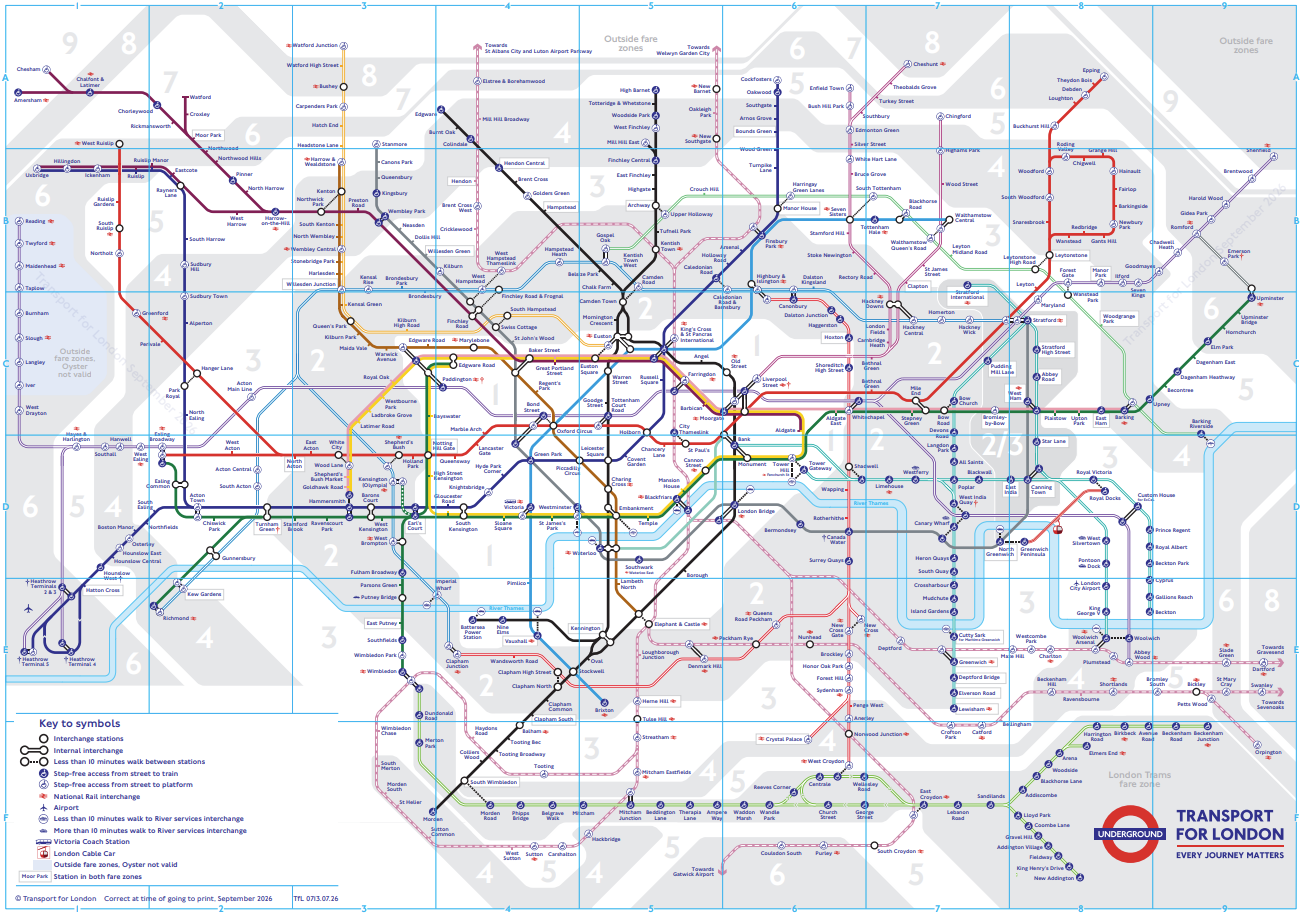
\includegraphics[width=\linewidth]{imagens/mapa_esquematico_londres.png}
        \caption{Rede do Metrô de Londres.}
        \label{fig:mapa_esquematico_londres}
    \end{subfigure}
    \hfill
    \begin{subfigure}[b]{0.48\textwidth}
        \centering
        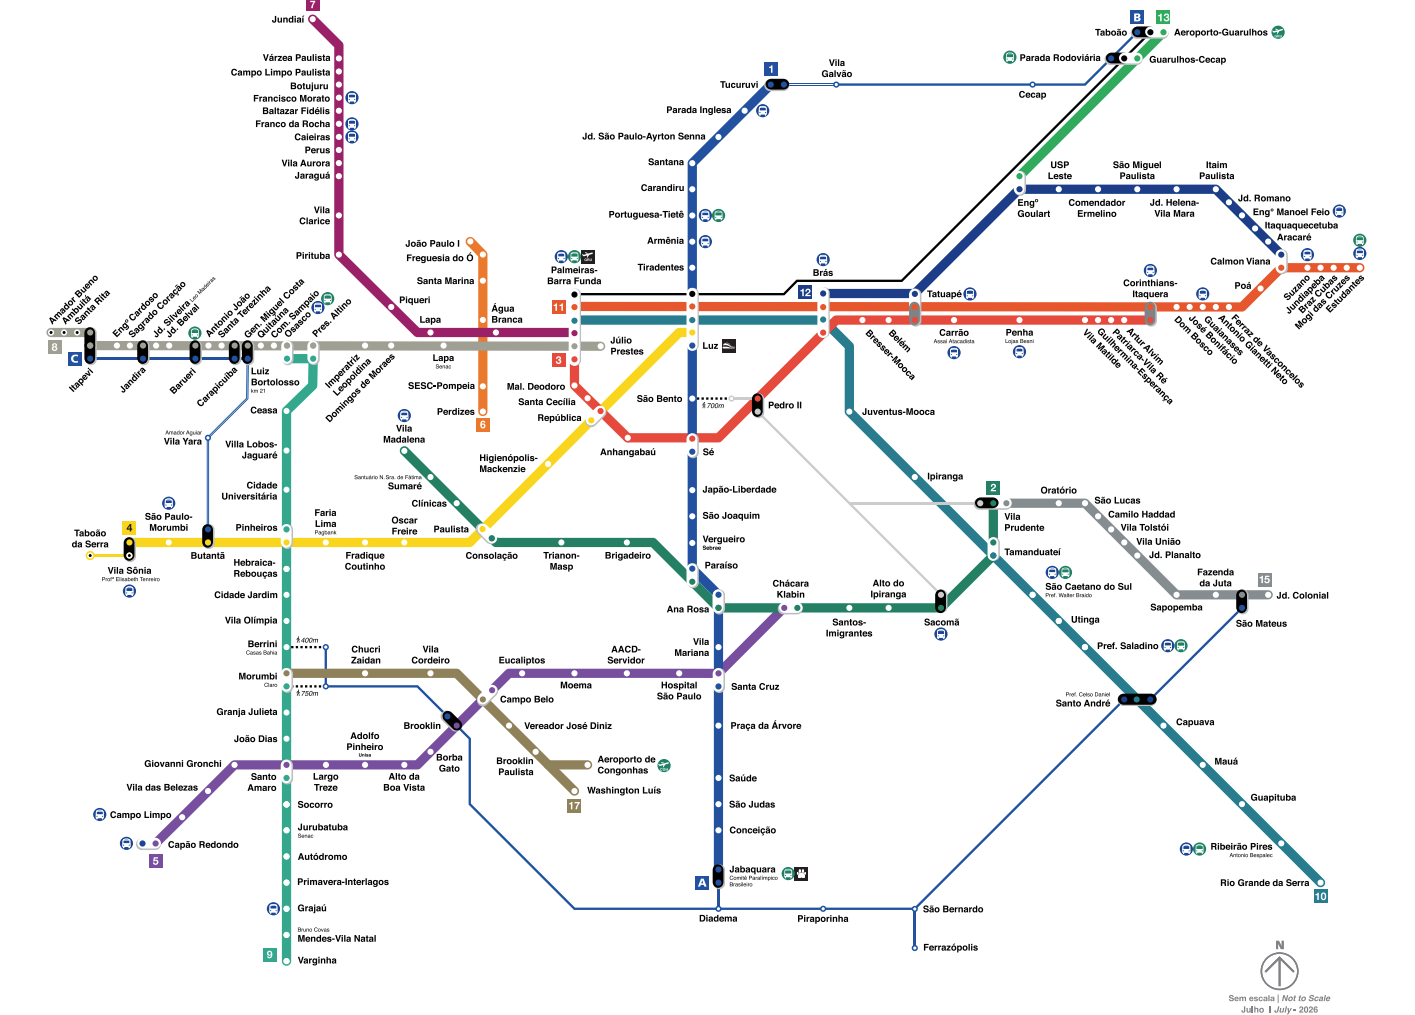
\includegraphics[width=\linewidth]{imagens/mapa_esquematico_saopaulo.png}
        \caption{Rede Metropolitana de São Paulo (Metrô e CPTM).}
        \label{fig:mapa_esquematico_saopaulo}
    \end{subfigure}
    \caption{Exemplos consagrados de mapas esquemáticos de transporte: em (a), a rede pioneira do metrô de Londres; em (b), a malha metropolitana sobre trilhos de São Paulo.}
    \label{fig:exemplos_mapas_esquematicos}
    \vspace{0.15cm}
    \par\raggedright\footnotesize\textit{Fonte: Adaptado de Transport for London~\cite{TfLTubeMap} e Companhia do Metropolitano de São Paulo~\cite{MetroSPMap}.}
\end{figure}


% Esta é a subseção mais importante deste capítulo. Apresente em detalhes o trabalho que é a base do seu TCC.
\subsection{O Modelo de Nöllenburg e Wolff}
% Comece explicando o problema que eles resolvem e a abordagem geral (MIP).
% Descreva as variáveis de decisão do modelo: o que elas representam? (e.g., coordenadas dos nós, direções das arestas).
% Detalhe as restrições rígidas (hard constraints): quais são elas e o que garantem? (e.g., topologia, geometria octolinear, não sobreposição).
% Explique a função objetivo e as restrições flexíveis (soft constraints): o que o modelo tenta otimizar? (e.g., minimizar o número de curvas, manter o comprimento das arestas uniforme, manter a proximidade com a geografia original).

Dadas as propriedades que dão ao mapa uma melhor legibilidade, Nöllenburg e Wolff propuseram um modelo de Programação Inteira Mista (MIP) que as transformam em equações lineares de otimização, separando-as em \textit{hard constraint} que são restrições que o modelo não pode permitir que sejam quebradas como por exemplo a octilinearidade do mapa, a ordem circular dos vértices vizinhos, o tamanho mínimo de arestas e o cruzamento de arestas indevido, e \textit{soft constraint} que são restrições cuja quebra resulta em uma penalidade e então é feito uma otimização de minimização destas penalidades, no caso o que se está minimizando são: dobras nas arestas, diferença de posição relativa, isto é, a diferença entre o ângulo original e o resultante, e o tamanho das arestas.

Para garantir a octilinearidade, o modelo emprega um sistema de coordenadas específico, apresentado na Figura~\ref{fig:nollenburg_coords_sec}(a). Nele, para cada vértice $v$, são definidas as variáveis inteiras $(x(v), y(v))$, que representam as coordenadas cartesianas na grade discreta, e as expressões lineares derivadas $z_1(v) = (x(v) + y(v))/2$ e $z_2(v) = (x(v) - y(v))/2$, as quais atuam como coordenadas rotacionadas e permitem tratar os eixos diagonais com a mesma linearidade dos eixos ortogonais. Com base nessas coordenadas, o plano em torno de cada nó $u$ é particionado em oito setores angulares de 45°, indexados de 0 a 7, conforme ilustrado na Figura~\ref{fig:nollenburg_coords_sec}(b).

A relação angular original entre um nó $u$ e seu vizinho $v$ é mapeada no setor correspondente por meio da constante $\text{sec}_u(v)$. A fim de permitir um leve desvio em relação à geografia original e conceder flexibilidade ao solver, o modelo incorpora variáveis binárias auxiliares, denotadas por $\alpha_i(u, v)$, que conferem a liberdade de inclinar uma aresta para um setor imediatamente adjacente (no sentido horário ou anti-horário). Por fim, a variável $\text{dir}(u, v)$ é utilizada para codificar a direção final octilinear atribuída a cada aresta no layout resultante.

\begin{figure}[H]
    \centering
    \begin{subfigure}[b]{0.42\textwidth}
        \centering
        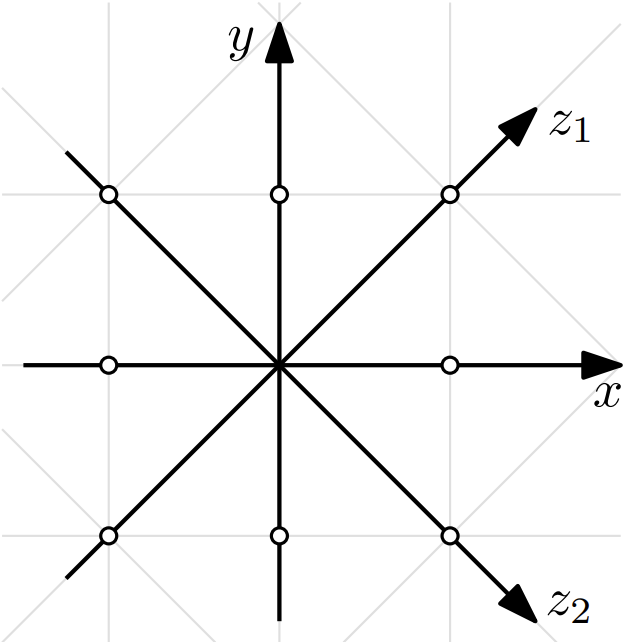
\includegraphics[width=0.85\linewidth]{imagens/nollenburg-coords.png}
        \caption{Sistema de coordenadas octilineares.}
        \label{fig:nollenburg_coords}
    \end{subfigure}
    \hspace{0.06\textwidth}
    \begin{subfigure}[b]{0.42\textwidth}
        \centering
        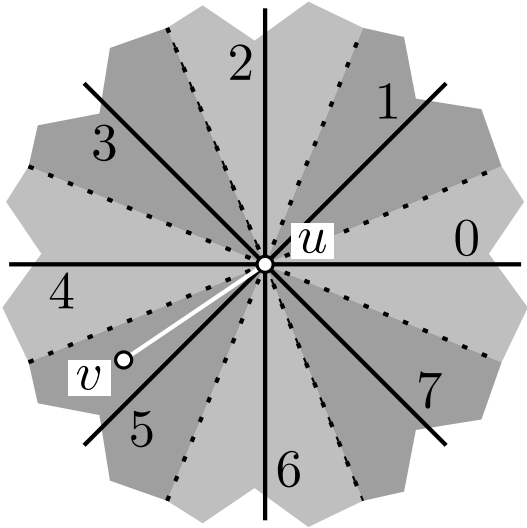
\includegraphics[width=0.85\linewidth]{imagens/nollenburg-sec.png}
        \caption{Setores angulares com $\text{sec}_u(v) = 5$.}
        \label{fig:nollenburg_sec}
    \end{subfigure}
    \caption{Fundamentos geométricos do modelo de Nöllenburg e Wolff: em (a), os eixos de coordenadas octilineares ($x, y, z_1, z_2$); em (b), a divisão do plano em oito setores angulares centrados em $u$, ilustrando o mapeamento de um nó vizinho $v$ no setor $\text{sec}_u(v) = 5$.}
    \label{fig:nollenburg_coords_sec}
    \vspace{0.15cm}
    \par\raggedright\footnotesize\textit{Fonte: Nöllenburg e Wolff~\cite{Nollenburg}.}
\end{figure}



A Equação~\ref{eq:alpha_sum} garante que cada aresta seja atribuída a exatamente um desvio angular, onde $\alpha_{\text{prec}}$ indica um movimento no sentido anti-horário, $\alpha_{\text{orig}}$ mantém a angulação original e $\alpha_{\text{succ}}$ representa um movimento no sentido horário. As equações em~\ref{eq:dir_calc} definem a direção final da aresta com base no setor original e no desvio escolhido. Finalmente, um subconjunto das restrições que forçam as coordenadas dos vértices a respeitarem a direção octilinear selecionada é mostrado em~\ref{eq:octi_coords}, onde $M$ é uma constante grande (Big M) e $\ell_{uv}$ é o comprimento mínimo da aresta.

\begin{equation}
\alpha_{\text{prec}}(u, v) + \alpha_{\text{orig}}(u, v) + \alpha_{\text{succ}}(u, v) = 1 \quad \forall (u, v) \in E.
\label{eq:alpha_sum}
\end{equation}

\begin{align}
\text{dir}(u, v) &= \sum_{i \in \{\text{prec,orig,succ}\}} \text{sec}_i^u(v) \cdot \alpha_i(u, v) && \forall (u, v) \in E, \label{eq:dir_calc} \\
\text{dir}(v, u) &= \sum_{i \in \{\text{prec,orig,succ}\}} \text{sec}_i^v(u) \cdot \alpha_i(u, v) && \forall (u, v) \in E. \nonumber
\end{align}

\begin{align}
\forall (u, v) \in E, \quad &\forall i \in \{\text{prec}, \text{orig}, \text{succ}\}: \label{eq:octi_coords} \\[0.4em]
\text{Se } \text{sec}_i^u(v) = 0 \text{ (Leste):} \quad & \left\{ \begin{aligned}
y(u) - y(v) &\le M(1 - \alpha_i(u, v)), \\
y(u) - y(v) &\ge -M(1 - \alpha_i(u, v)), \\
x(v) - x(u) &\ge \ell_{uv} - M(1 - \alpha_i(u, v)),
\end{aligned} \right. \nonumber \\[0.4em]
\text{Se } \text{sec}_i^u(v) = 1 \text{ (Nordeste):} \quad & \left\{ \begin{aligned}
z_2(u) - z_2(v) &\le M(1 - \alpha_i(u, v)), \\
z_2(u) - z_2(v) &\ge -M(1 - \alpha_i(u, v)), \\
z_1(v) - z_1(u) &\ge \ell_{uv} - M(1 - \alpha_i(u, v)),
\end{aligned} \right. \nonumber \\[0.4em]
\text{Se } \text{sec}_i^u(v) = 2 \text{ (Norte):} \quad & \left\{ \begin{aligned}
x(u) - x(v) &\le M(1 - \alpha_i(u, v)), \\
x(u) - x(v) &\ge -M(1 - \alpha_i(u, v)), \\
y(v) - y(u) &\ge \ell_{uv} - M(1 - \alpha_i(u, v)),
\end{aligned} \right. \nonumber \\[0.4em]
\text{Se } \text{sec}_i^u(v) = 3 \text{ (Noroeste):} \quad & \left\{ \begin{aligned}
z_1(u) - z_1(v) &\le M(1 - \alpha_i(u, v)), \\
z_1(u) - z_1(v) &\ge -M(1 - \alpha_i(u, v)), \\
z_2(u) - z_2(v) &\ge \ell_{uv} - M(1 - \alpha_i(u, v)),
\end{aligned} \right. \nonumber \\[0.4em]
\text{Se } \text{sec}_i^u(v) = 4 \text{ (Oeste):} \quad & \left\{ \begin{aligned}
y(u) - y(v) &\le M(1 - \alpha_i(u, v)), \\
y(u) - y(v) &\ge -M(1 - \alpha_i(u, v)), \\
x(u) - x(v) &\ge \ell_{uv} - M(1 - \alpha_i(u, v)),
\end{aligned} \right. \nonumber \\[0.4em]
\text{Se } \text{sec}_i^u(v) = 5 \text{ (Sudoeste):} \quad & \left\{ \begin{aligned}
z_2(u) - z_2(v) &\le M(1 - \alpha_i(u, v)), \\
z_2(u) - z_2(v) &\ge -M(1 - \alpha_i(u, v)), \\
z_1(u) - z_1(v) &\ge \ell_{uv} - M(1 - \alpha_i(u, v)),
\end{aligned} \right. \nonumber \\[0.4em]
\text{Se } \text{sec}_i^u(v) = 6 \text{ (Sul):} \quad & \left\{ \begin{aligned}
x(u) - x(v) &\le M(1 - \alpha_i(u, v)), \\
x(u) - x(v) &\ge -M(1 - \alpha_i(u, v)), \\
y(u) - y(v) &\ge \ell_{uv} - M(1 - \alpha_i(u, v)),
\end{aligned} \right. \nonumber \\[0.4em]
\text{Se } \text{sec}_i^u(v) = 7 \text{ (Sudeste):} \quad & \left\{ \begin{aligned}
z_1(u) - z_1(v) &\le M(1 - \alpha_i(u, v)), \\
z_1(u) - z_1(v) &\ge -M(1 - \alpha_i(u, v)), \\
z_2(v) - z_2(u) &\ge \ell_{uv} - M(1 - \alpha_i(u, v)).
\end{aligned} \right. \nonumber
\end{align}

A preservação da ordem circular das arestas em torno de um vértice é outra restrição fundamental. Para cada vértice $v$ com grau $deg(v) \ge 2$, seus vizinhos $u_1, \dots, u_{\text{deg}(v)}$ são ordenados no sentido anti-horário. O modelo então utiliza variáveis binárias $\beta_j(v)$ para indicar em qual par consecutivo de vizinhos ocorre a quebra de monotonicidade na transição do setor $7$ para o $0$. A Equação~\ref{eq:beta_sum} assegura que esse salto ocorra em uma única posição, enquanto as inequações em~\ref{eq:circular_order} forçam as direções das arestas a crescerem respeitando a ordem circular original.

\begin{equation}
\sum_{j=1}^{\text{deg}(v)} \beta_j(v) = 1 \quad \forall v \in V \mid \text{deg}(v) \ge 2.
\label{eq:beta_sum}
\end{equation}

\begin{align}
\text{dir}(v, u_1) &\le \text{dir}(v, u_2) - 1 + 8\beta_1(v), && \forall v \in V \mid \text{deg}(v) \ge 2 \label{eq:circular_order} \\
\text{dir}(v, u_2) &\le \text{dir}(v, u_3) - 1 + 8\beta_2(v), \nonumber \\
&\vdots \nonumber \\
\text{dir}(v, u_{\text{deg}(v)}) &\le \text{dir}(v, u_1) - 1 + 8\beta_{\text{deg}(v)}(v). \nonumber
\end{align}

Para evitar o cruzamento entre arestas, o modelo impõe uma restrição de separação espacial. A lógica consiste em garantir que, para qualquer par de arestas não adjacentes $e_1=(u_1, v_1)$ e $e_2=(u_2, v_2)$, suas caixas delimitadoras (bounding boxes) não se sobreponham. Isso é modelado forçando que os vértices de uma aresta estejam completamente de um lado da outra em pelo menos uma das oito direções octilineares. Variáveis binárias $\gamma_k(e_1, e_2)$ são introduzidas para selecionar em qual dessas direções a separação deve ocorrer. A Equação~\ref{eq:crossing_sum} força a escolha de pelo menos uma direção, e as inequações em~\ref{eq:crossing_coord} detalham como essa separação é imposta para cada uma das oito direções, onde $d_{\text{min}}$ é uma distância mínima.

\begin{equation}
\sum_{k \in \{\text{N,S,E,W,NE,NW,SE,SW}\}} \gamma_k(e_1, e_2) \ge 1 \quad \forall e_1, e_2 \in E.
\label{eq:crossing_sum}
\end{equation}

\begin{align}
\forall e_1 = (u_1, v_1), \quad &\forall e_2 = (u_2, v_2) \in E: \label{eq:crossing_coord} \\[0.4em]
\text{Direção Leste ($\gamma_{\text{E}}$):} \quad & \left\{ \begin{aligned}
x(u_2) - x(u_1) &\le M(1 - \gamma_{\text{E}}(e_1, e_2)) - d_{\text{min}}, \\
x(u_2) - x(v_1) &\le M(1 - \gamma_{\text{E}}(e_1, e_2)) - d_{\text{min}}, \\
x(v_2) - x(u_1) &\le M(1 - \gamma_{\text{E}}(e_1, e_2)) - d_{\text{min}}, \\
x(v_2) - x(v_1) &\le M(1 - \gamma_{\text{E}}(e_1, e_2)) - d_{\text{min}},
\end{aligned} \right. \nonumber \\[0.4em]
\text{Direção Nordeste ($\gamma_{\text{NE}}$):} \quad & \left\{ \begin{aligned}
z_1(u_2) - z_1(u_1) &\le M(1 - \gamma_{\text{NE}}(e_1, e_2)) - d_{\text{min}}, \\
z_1(u_2) - z_1(v_1) &\le M(1 - \gamma_{\text{NE}}(e_1, e_2)) - d_{\text{min}}, \\
z_1(v_2) - z_1(u_1) &\le M(1 - \gamma_{\text{NE}}(e_1, e_2)) - d_{\text{min}}, \\
z_1(v_2) - z_1(v_1) &\le M(1 - \gamma_{\text{NE}}(e_1, e_2)) - d_{\text{min}},
\end{aligned} \right. \nonumber \\[0.4em]
\text{Direção Norte ($\gamma_{\text{N}}$):} \quad & \left\{ \begin{aligned}
y(u_2) - y(u_1) &\le M(1 - \gamma_{\text{N}}(e_1, e_2)) - d_{\text{min}}, \\
y(u_2) - y(v_1) &\le M(1 - \gamma_{\text{N}}(e_1, e_2)) - d_{\text{min}}, \\
y(v_2) - y(u_1) &\le M(1 - \gamma_{\text{N}}(e_1, e_2)) - d_{\text{min}}, \\
y(v_2) - y(v_1) &\le M(1 - \gamma_{\text{N}}(e_1, e_2)) - d_{\text{min}},
\end{aligned} \right. \nonumber \\[0.4em]
\text{Direção Noroeste ($\gamma_{\text{NW}}$):} \quad & \left\{ \begin{aligned}
-z_2(u_2) + z_2(u_1) &\le M(1 - \gamma_{\text{NW}}(e_1, e_2)) - d_{\text{min}}, \\
-z_2(u_2) + z_2(v_1) &\le M(1 - \gamma_{\text{NW}}(e_1, e_2)) - d_{\text{min}}, \\
-z_2(v_2) + z_2(u_1) &\le M(1 - \gamma_{\text{NW}}(e_1, e_2)) - d_{\text{min}}, \\
-z_2(v_2) + z_2(v_1) &\le M(1 - \gamma_{\text{NW}}(e_1, e_2)) - d_{\text{min}},
\end{aligned} \right. \nonumber \\[0.4em]
\text{Direção Oeste ($\gamma_{\text{W}}$):} \quad & \left\{ \begin{aligned}
-x(u_2) + x(u_1) &\le M(1 - \gamma_{\text{W}}(e_1, e_2)) - d_{\text{min}}, \\
-x(u_2) + x(v_1) &\le M(1 - \gamma_{\text{W}}(e_1, e_2)) - d_{\text{min}}, \\
-x(v_2) + x(u_1) &\le M(1 - \gamma_{\text{W}}(e_1, e_2)) - d_{\text{min}}, \\
-x(v_2) + x(v_1) &\le M(1 - \gamma_{\text{W}}(e_1, e_2)) - d_{\text{min}},
\end{aligned} \right. \nonumber \\[0.4em]
\text{Direção Sudoeste ($\gamma_{\text{SW}}$):} \quad & \left\{ \begin{aligned}
-z_1(u_2) + z_1(u_1) &\le M(1 - \gamma_{\text{SW}}(e_1, e_2)) - d_{\text{min}}, \\
-z_1(u_2) + z_1(v_1) &\le M(1 - \gamma_{\text{SW}}(e_1, e_2)) - d_{\text{min}}, \\
-z_1(v_2) + z_1(u_1) &\le M(1 - \gamma_{\text{SW}}(e_1, e_2)) - d_{\text{min}}, \\
-z_1(v_2) + z_1(v_1) &\le M(1 - \gamma_{\text{SW}}(e_1, e_2)) - d_{\text{min}},
\end{aligned} \right. \nonumber \\[0.4em]
\text{Direção Sul ($\gamma_{\text{S}}$):} \quad & \left\{ \begin{aligned}
-y(u_2) + y(u_1) &\le M(1 - \gamma_{\text{S}}(e_1, e_2)) - d_{\text{min}}, \\
-y(u_2) + y(v_1) &\le M(1 - \gamma_{\text{S}}(e_1, e_2)) - d_{\text{min}}, \\
-y(v_2) + y(u_1) &\le M(1 - \gamma_{\text{S}}(e_1, e_2)) - d_{\text{min}}, \\
-y(v_2) + y(v_1) &\le M(1 - \gamma_{\text{S}}(e_1, e_2)) - d_{\text{min}},
\end{aligned} \right. \nonumber \\[0.4em]
\text{Direção Sudeste ($\gamma_{\text{SE}}$):} \quad & \left\{ \begin{aligned}
z_2(u_2) - z_2(u_1) &\le M(1 - \gamma_{\text{SE}}(e_1, e_2)) - d_{\text{min}}, \\
z_2(u_2) - z_2(v_1) &\le M(1 - \gamma_{\text{SE}}(e_1, e_2)) - d_{\text{min}}, \\
z_2(v_2) - z_2(u_1) &\le M(1 - \gamma_{\text{SE}}(e_1, e_2)) - d_{\text{min}}, \\
z_2(v_2) - z_2(v_1) &\le M(1 - \gamma_{\text{SE}}(e_1, e_2)) - d_{\text{min}}.
\end{aligned} \right. \nonumber
\end{align}

Passando para as restrições flexíveis (soft constraints), que compõem a função objetivo, um dos principais componentes é a minimização de curvas. Para cada par de arestas adjacentes $(u, v)$ e $(v, w)$ em uma rota $L$, uma variável $\bd(u, v, w)$ é introduzida para quantificar a penalidade da curva no vértice $v$. O custo total associado às curvas, $C_{\text{bends}}$, é então a soma dessas penalidades sobre todas as rotas, conforme a Equação~\ref{eq:cost_bends}.

\begin{equation}
C_{\text{bends}} = \sum_{L \in \mathcal{L}} \sum_{(u,v),(v,w) \in L} \bd(u, v, w).
\label{eq:cost_bends}
\end{equation}

A magnitude da curva é calculada com base na diferença, $\Delta_{\text{dir}}(u,v,w)$, entre as direções octilineares $\text{dir}(u, v)$ e $\text{dir}(v, w)$. Como o sistema de direções é cíclico (módulo 8), a menor ``distância'' angular entre duas direções é dada pela Equação~\ref{eq:bend_calc}. Esta função não-linear é então modelada no MIP por meio de variáveis binárias auxiliares $\delta_1$ e $\delta_2$ e do conjunto de inequações em~\ref{eq:bend_linearization}.

\begin{equation}
\begin{aligned}
&\forall L \in \mathcal{L}, \; \forall (u,v),(v,w) \in L: \\
&\bd(u, v, w) = \min\{|\Delta_{\text{dir}}(u,v,w)|, 8 - |\Delta_{\text{dir}}(u,v,w)|\}.
\end{aligned}
\label{eq:bend_calc}
\end{equation}

\begin{align}
\forall L \in \mathcal{L}, \quad &\forall (u,v),(v,w) \in L: \label{eq:bend_linearization} \\
-\bd(u, v, w) &\le \Delta_{\text{dir}}(u,v,w) - 8\delta_1(u, v, w) + 8\delta_2(u, v, w), \nonumber \\
\bd(u, v, w) &\ge \Delta_{\text{dir}}(u,v,w) - 8\delta_1(u, v, w) + 8\delta_2(u, v, w). \nonumber
\end{align}

A segunda penalidade da função objetivo visa preservar a posição relativa das arestas, mantendo a geometria geral do mapa. Para cada aresta $(u,v)$, uma variável de penalidade binária $\rpos(u,v)$ é ativada se a direção final $\text{dir}(u,v)$ divergir da direção do setor original $\text{sec}_u(v)$. O custo total, $C_{\text{rpos}}$, é a soma dessas penalidades (Equação~\ref{eq:cost_rpos}). A relação entre a penalidade e a mudança de direção é linearizada através da inequação em~\ref{eq:rpos_linearization}, onde $M$ é uma constante grande.

\begin{equation}
C_{\text{rpos}} = \sum_{(u,v) \in E} \rpos(u, v).
\label{eq:cost_rpos}
\end{equation}

\begin{equation}
-M \cdot \rpos(u,v) \le \text{dir}(u, v) - \text{sec}_u(v) \le M \cdot \rpos(u,v) \quad \forall (u, v) \in E.
\label{eq:rpos_linearization}
\end{equation}
 
Por fim, a última penalidade na função objetivo busca minimizar o comprimento total das arestas. Para cada aresta $(u,v)$, uma variável $\lambda(u,v)$ é introduzida para representar um limite superior (upper bound) para seu comprimento. O custo total associado, $C_{\text{len}}$, é a soma dessas variáveis, como mostra a Equação~\ref{eq:cost_len}. A relação entre $\lambda(u,v)$ e as coordenadas dos vértices é estabelecida por um conjunto de inequações (Equação~\ref{eq:len_linearization}), que efetivamente modelam o comprimento de Manhattan da aresta.

\begin{equation}
C_{\text{len}} = \sum_{(u,v) \in E} \lambda(u, v).
\label{eq:cost_len}
\end{equation}

\begin{align}
x(u) - x(v) &\le \lambda(u,v), && \forall (u, v) \in E \label{eq:len_linearization} \\
-x(u) + x(v) &\le \lambda(u,v), \nonumber \\
y(u) - y(v) &\le \lambda(u,v), \nonumber \\
-y(u) + y(v) &\le \lambda(u,v). \nonumber
\end{align}

Com todas as penalidades devidamente formuladas, a função objetivo global do modelo é definida como uma combinação linear ponderada desses três componentes, conforme apresentado na Equação~\ref{eq:funcao_objetivo_nollenburg}. Os coeficientes $w_{\text{bends}}$, $w_{\text{rpos}}$ e $w_{\text{len}}$ correspondem aos pesos atribuídos a cada penalidade, permitindo priorizar determinados critérios estéticos ou topológicos durante o processo de otimização.

\begin{equation}
\min \quad w_{\text{bends}} \cdot C_{\text{bends}} + w_{\text{rpos}} \cdot C_{\text{rpos}} + w_{\text{len}} \cdot C_{\text{len}}.
\label{eq:funcao_objetivo_nollenburg}
\end{equation}
 
% Explique o que é o padrão GTFS (General Transit Feed Specification).
% Descreva a estrutura dos dados e quais arquivos são relevantes para o seu trabalho.
% Detalhe a informação que você extrai de cada arquivo: `routes.txt`, `stops.txt`, `trips.txt`, `shapes.txt`.
% Isso fará a ponte para o seu capítulo de Metodologia, onde você explica como processou esses dados.
\section{Padrão de Dados GTFS}

O padrão \textit{General Transit Feed Specification} (GTFS) é um formato de dados aberto, originalmente desenvolvido pela Google, que se tornou o padrão internacional de fato para a divulgação de dados operacionais e geográficos de transporte público em arquivos no formato de valores separados por vírgula (CSV). Para este trabalho, foram utilizados os dados da rede de Porto Alegre fornecidos pela EPTC, com foco nos arquivos essenciais que permitem reconstruir a topologia e a geografia da malha de transporte. As Tabelas~\ref{tab:gtfs_routes} a~\ref{tab:gtfs_shapes} detalham os campos empregados em cada um desses arquivos.

O arquivo \texttt{routes.txt}, sumarizado na Tabela~\ref{tab:gtfs_routes}, cataloga o conjunto de linhas de ônibus em operação. Cada linha é identificada pelo campo \texttt{route\_id}, possuindo a denominação operacional (\texttt{route\_short\_name}) e o código de cor hexadecimal (\texttt{route\_color}), atributo fundamental para assegurar a distinção cromática dos múltiplos itinerários na renderização do mapa esquemático.

\begin{table}[H]
  \centering
  \caption{Campos relevantes do arquivo \texttt{routes.txt}.}
  \label{tab:gtfs_routes}
  \begin{tabular}{ll}
    \toprule
    \textbf{Campo} & \textbf{Descrição} \\
    \midrule
    \texttt{route\_id} & Identificador único da rota. \\
    \texttt{route\_short\_name} & Nome curto da rota (ex: ``T1'', ``272''). \\
    \texttt{route\_color} & Cor associada à rota para uso em mapas. \\
    \bottomrule
  \end{tabular}
\end{table}

O arquivo \texttt{trips.txt}, detalhado na Tabela~\ref{tab:gtfs_trips}, atua como a entidade relacional que conecta as linhas aos seus respectivos percursos físicos e operacionais. Cada registro descreve uma viagem específica \texttt{trip\_id}, associando-a à linha correspondente por meio da chave estrangeira \texttt{route\_id}. Adicionalmente, o arquivo especifica o sentido do deslocamento pelo atributo \texttt{direction\_id} (diferenciando viagens de ida e de volta) e vincula a viagem à sua geometria contínua mediante a chave estrangeira \texttt{shape\_id}.

\begin{table}[H]
  \centering
  \caption{Campos relevantes do arquivo \texttt{trips.txt}.}
  \label{tab:gtfs_trips}
  \begin{tabular}{ll}
    \toprule
    \textbf{Campo} & \textbf{Descrição} \\
    \midrule
    \texttt{trip\_id} & Identificador único da viagem. \\
    \texttt{route\_id} & Chave estrangeira para \texttt{routes.txt}. \\
    \texttt{shape\_id} & Chave estrangeira para \texttt{shapes.txt}. \\
    \texttt{direction\_id} & Sentido da viagem (e.g., ida ou volta). \\
    \bottomrule
  \end{tabular}
\end{table}

O arquivo \texttt{stops.txt}, apresentado na Tabela~\ref{tab:gtfs_stops}, relaciona todos os pontos físicos de embarque e desembarque atendidos pelo sistema. Cada parada é unicamente definida pelo atributo \texttt{stop\_id} e possui uma denominação textual no campo \texttt{stop\_name}. As coordenadas geográficas reais de cada ponto são informadas em \texttt{stop\_lat} e \texttt{stop\_lon}, constituindo os dados de posicionamento indispensáveis para a localização e para as operações de projeção geométrica.

\begin{table}[H]
  \centering
  \caption{Campos relevantes do arquivo \texttt{stops.txt}.}
  \label{tab:gtfs_stops}
  \begin{tabular}{ll}
    \toprule
    \textbf{Campo} & \textbf{Descrição} \\
    \midrule
    \texttt{stop\_id} & Identificador único da parada. \\
    \texttt{stop\_name} & Nome da parada para exibição. \\
    \texttt{stop\_lat} & Latitude da parada (coordenada geográfica). \\
    \texttt{stop\_lon} & Longitude da parada (coordenada geográfica). \\
    \bottomrule
  \end{tabular}
\end{table}

O arquivo \texttt{stop\_times.txt}, sintetizado na Tabela~\ref{tab:gtfs_stoptimes}, estabelece o encadeamento operacional entre as viagens e as paradas ao longo do tempo e do espaço. A tabela associa cada viagem (\texttt{trip\_id}) à parada atendida (\texttt{stop\_id}) e estipula a ordem estrita em que os veículos percorrem cada ponto mediante o índice sequencial \texttt{stop\_sequence}. Essa estrutura viabiliza a reconstrução direta da sequência de viagens e a geração do grafo baseado em conexões diretas entre paradas consecutivas.

\begin{table}[H]
  \centering
  \caption{Campos relevantes do arquivo \texttt{stop\_times.txt}.}
  \label{tab:gtfs_stoptimes}
  \begin{tabular}{ll}
    \toprule
    \textbf{Campo} & \textbf{Descrição} \\
    \midrule
    \texttt{trip\_id} & Chave estrangeira para \texttt{trips.txt}. \\
    \texttt{stop\_id} & Chave estrangeira para \texttt{stops.txt}. \\
    \texttt{stop\_sequence} & Ordem da parada dentro de uma viagem. \\
    \bottomrule
  \end{tabular}
\end{table}

Por fim, o arquivo \texttt{shapes.txt}, descrito na Tabela~\ref{tab:gtfs_shapes}, define a geometria detalhada do traçado percorrido pelas linhas na infraestrutura viária urbana. Cada alinhamento espacial é indexado por \texttt{shape\_id} e formado por uma série ordenada de pontos geográficos (\texttt{shape\_pt\_lat} e \texttt{shape\_pt\_lon}), cuja sucessão física é governada pelo campo \texttt{shape\_pt\_sequence}. Esse arquivo fornece o alinhamento contínuo das vias necessário para a construção do esqueleto estrutural (\textit{backbone}) da rede.

\begin{table}[H]
  \centering
  \caption{Campos relevantes do arquivo \texttt{shapes.txt}.}
  \label{tab:gtfs_shapes}
  \begin{tabular}{ll}
    \toprule
    \textbf{Campo} & \textbf{Descrição} \\
    \midrule
    \texttt{shape\_id} & Identificador único do traçado (\textit{shape}). \\
    \texttt{shape\_pt\_lat} & Latitude do ponto geográfico do traçado. \\
    \texttt{shape\_pt\_lon} & Longitude do ponto geográfico do traçado. \\
    \texttt{shape\_pt\_sequence} & Ordem sequencial do ponto ao longo do traçado. \\
    \bottomrule
  \end{tabular}
\end{table}

A combinação desses arquivos permite reconstruir tanto a topologia quanto a geometria da rede de transporte, estruturando-se segundo o modelo relacional apresentado na Figura~\ref{fig:diagrama_relacional_gtfs}. O arquivo \texttt{routes.txt} define as linhas do sistema, enquanto o \texttt{trips.txt} atua como a entidade central de junção, especificando as viagens associadas a cada linha. A partir dessas viagens, existem duas abordagens possíveis para a modelagem do traçado: a primeira utiliza a chave estrangeira \texttt{trip\_id} para associar a viagem ao arquivo \texttt{stop\_times.txt}, gerando um grafo baseado na conexão direta entre paradas sucessivas; a segunda utiliza a chave estrangeira \texttt{shape\_id} para consultar o arquivo \texttt{shapes.txt}, gerando um grafo fundamentado no traçado geográfico real das vias. Enquanto a primeira abordagem enfatiza os pontos de embarque e desembarque atendidos pelos ônibus, a segunda preserva com maior fidelidade a continuidade física e topológica dos itinerários. A lógica de construção em ambos os casos é semelhante, empregando-se os campos de ordenação \texttt{stop\_sequence} e \texttt{shape\_pt\_sequence}, respectivamente, para encadear a sequência de vértices que compõem cada rota no grafo. A escolha entre essas duas estratégias define a estrutura da malha de entrada e impacta diretamente a complexidade e o desempenho da otimização via modelo MIP.

\begin{figure}[H]
  \centering
  \caption{Diagrama relacional das tabelas GTFS utilizadas na modelagem da rede.}
  \label{fig:diagrama_relacional_gtfs}
  \vspace{0.3cm}
  \resizebox{0.95\textwidth}{!}{%
  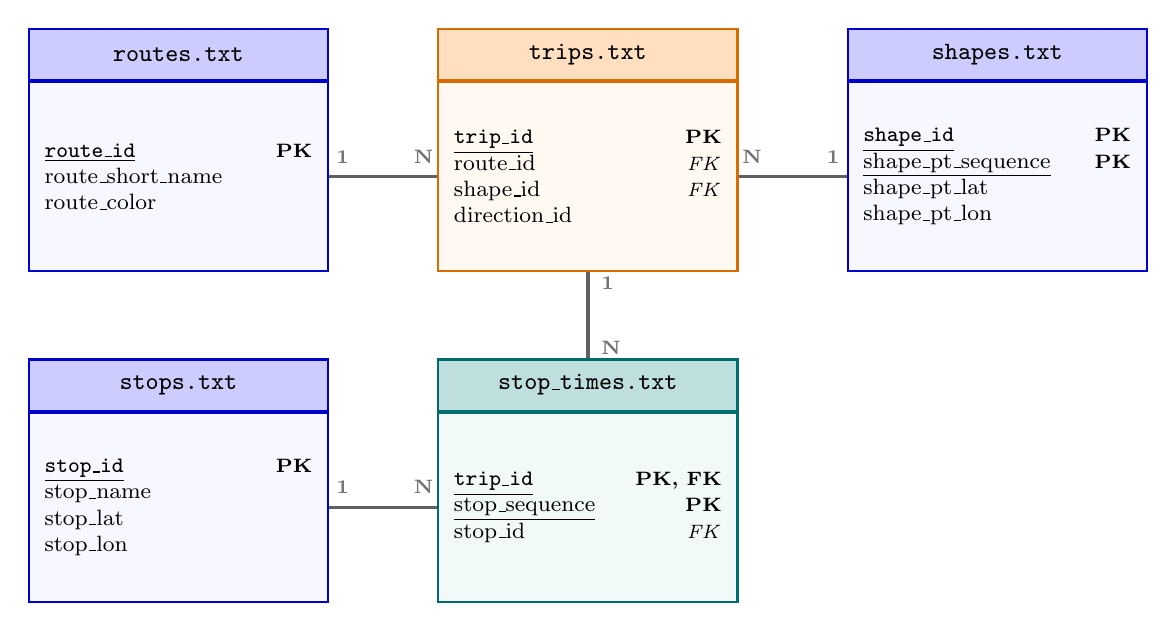
\begin{tikzpicture}[
    table_header/.style={
      rectangle,
      draw=blue!80!black,
      fill=blue!20,
      thick,
      minimum width=3.8cm,
      minimum height=0.65cm,
      font=\bfseries\small,
      align=center
    },
    table_body/.style={
      rectangle,
      draw=blue!80!black,
      fill=blue!3,
      thick,
      minimum width=3.8cm,
      minimum height=2.4cm,
      align=left,
      text width=3.4cm,
      font=\footnotesize\ttfamily,
      inner sep=5pt
    },
    rel_edge/.style={
      very thick,
      gray!75!black
    },
    card_label/.style={
      font=\scriptsize\bfseries,
      text=gray!90!black
    }
  ]
    % --- LINHA 1 (Superior) ---
    % routes.txt
    \node[table_header] (routes_h) at (0, 3.8) {\texttt{routes.txt}};
    \node[table_body, below=0pt of routes_h] (routes_b) {
      \underline{route\_id} \hfill \normalfont\textbf{\scriptsize PK} \\
      route\_short\_name \\
      route\_color
    };

    % trips.txt (Central)
    \node[table_header, fill=orange!25, draw=orange!85!black] (trips_h) at (5.2, 3.8) {\texttt{trips.txt}};
    \node[table_body, fill=orange!5, draw=orange!85!black, below=0pt of trips_h] (trips_b) {
      \underline{trip\_id} \hfill \normalfont\textbf{\scriptsize PK} \\
      route\_id \hfill \normalfont\textit{\scriptsize FK} \\
      shape\_id \hfill \normalfont\textit{\scriptsize FK} \\
      direction\_id
    };

    % shapes.txt
    \node[table_header] (shapes_h) at (10.4, 3.8) {\texttt{shapes.txt}};
    \node[table_body, below=0pt of shapes_h] (shapes_b) {
      \underline{shape\_id} \hfill \normalfont\textbf{\scriptsize PK} \\
      \underline{shape\_pt\_sequence} \hfill \normalfont\textbf{\scriptsize PK} \\
      shape\_pt\_lat \\
      shape\_pt\_lon
    };

    % --- LINHA 2 (Inferior) ---
    % stops.txt
    \node[table_header] (stops_h) at (0, -0.4) {\texttt{stops.txt}};
    \node[table_body, below=0pt of stops_h] (stops_b) {
      \underline{stop\_id} \hfill \normalfont\textbf{\scriptsize PK} \\
      stop\_name \\
      stop\_lat \\
      stop\_lon
    };

    % stop_times.txt
    \node[table_header, fill=teal!25, draw=teal!85!black] (stoptimes_h) at (5.2, -0.4) {\texttt{stop\_times.txt}};
    \node[table_body, fill=teal!5, draw=teal!85!black, below=0pt of stoptimes_h] (stoptimes_b) {
      \underline{trip\_id} \hfill \normalfont\textbf{\scriptsize PK, FK} \\
      \underline{stop\_sequence} \hfill \normalfont\textbf{\scriptsize PK} \\
      stop\_id \hfill \normalfont\textit{\scriptsize FK}
    };

    % --- RELACIONAMENTOS (Arestas não direcionadas com cardinalidades) ---
    % 1) routes (1) -- (N) trips
    \draw[rel_edge] (routes_b.east) -- (trips_b.west |- routes_b.east)
      node[card_label, very near start, above=1pt] {1}
      node[card_label, very near end, above=1pt] {N};

    % 2) shapes (1) -- (N) trips
    \draw[rel_edge] (shapes_b.west) -- (trips_b.east |- shapes_b.west)
      node[card_label, very near start, above=1pt] {1}
      node[card_label, very near end, above=1pt] {N};

    % 3) trips (1) -- (N) stop_times
    \draw[rel_edge] (trips_b.south) -- (stoptimes_h.north -| trips_b.south)
      node[card_label, very near start, right=1pt] {1}
      node[card_label, very near end, right=1pt] {N};

    % 4) stops (1) -- (N) stop_times
    \draw[rel_edge] (stops_b.east) -- (stoptimes_b.west |- stops_b.east)
      node[card_label, very near start, above=1pt] {1}
      node[card_label, very near end, above=1pt] {N};

  \end{tikzpicture}%
  }
\end{figure}

\chapter{Metodologia e Desenvolvimento}
\label{cap:metodologia}

Este capítulo descreve a metodologia e as decisões de projeto adotadas para a concepção do pipeline de geração automatizada de mapas esquemáticos da rede de ônibus de Porto Alegre. A abordagem proposta transforma os dados brutos no formato GTFS~\cite{gtfs_spec} em uma estrutura de grafo apta a representações octilineares simplificadas, formulando e resolvendo o problema de layout automático por meio de Programação Inteira Mista (MIP).

Para alcançar esse objetivo, o restante deste capítulo organiza-se acompanhando o encadeamento das etapas do fluxo desenvolvido. Inicialmente, a Seção~\ref{sec:arquitetura} apresenta a arquitetura modular da solução e a divisão de responsabilidades entre os componentes do sistema. Em seguida, a Seção~\ref{sec:preprocessamento} detalha a ingestão dos dados operacionais e geográficos das linhas e a construção de uma malha topológica simplificada, com o intuito de mitigar a complexidade da rede a ser processada. Na sequência, a Seção~\ref{sec:modelo_otimizacao} expõe a formulação matemática do modelo MIP adaptado ao transporte rodoviário urbano, abordando o relaxamento de restrições de cruzamento e o algoritmo de correção iterativa de distorções geométricas. Por fim, a Seção~\ref{sec:exportacao} descreve a estruturação e exportação dos resultados no padrão GraphML~\cite{brandes2010graph} para renderização e avaliação qualitativa em interface gráfica.

A seleção das tecnologias empregadas em cada etapa foi guiada sobretudo por requisitos de eficiência computacional, desempenho e escalabilidade. A linguagem Julia~\cite{bezanson2017julia} foi adotada para a implementação dos algoritmos de manipulação de grafos e integração do modelo matemático, atuando em conjunto com o solver comercial IBM ILOG CPLEX (versão~22.1.1.0)~\cite{cplex2022} para a resolução do problema. Por sua vez, a etapa de renderização e inspeção visual dos mapas gerados baseou-se na interface gráfica (GUI) em Java desenvolvida por Nöllenburg, cuja compatibilidade foi assegurada mediante a geração padronizada de arquivos GraphML.



\section{Arquitetura da Solução e Fluxo Modular}
\label{sec:arquitetura}

Para viabilizar a execução do pipeline de forma extensível e organizada, a solução foi projetada sob uma arquitetura modular baseada em scripts e pacotes na linguagem Julia. O fluxo de dados e a divisão de responsabilidades entre os componentes do sistema estão ilustrados na Figura~\ref{fig:fluxo_arquitetura}. A execução é coordenada pelo script orquestrador \texttt{map.jl}, que gerencia o ciclo de vida completo do processo. Inicialmente, o módulo \texttt{data\_parser.jl} é acionado para realizar a leitura dos arquivos GTFS brutos (\texttt{routes.txt}, \texttt{trips.txt}, \texttt{stops.txt}, \texttt{stop\_times.txt} e \texttt{shapes.txt}), aplicando os filtros e as rotinas de simplificação topológica para gerar um grafo de entrada tratável. Em seguida, o grafo estruturado é encaminhado ao módulo \texttt{mip\_constraints.jl}, onde o modelo matemático de otimização é instanciado com todas as variáveis, restrições e funções de custo octilineares. O orquestrador então submete o modelo ao solver CPLEX, que executa a resolução das variáveis de posicionamento e direção dos vértices e arestas. Uma vez obtidas as coordenadas otimizadas, o controle retorna ao fluxo principal, e o módulo \texttt{gtfs\_to\_xml.jl} é encarregado de consolidar a geometria da rede e os metadados das linhas de ônibus, exportando o resultado final no formato padronizado GraphML. Adicionalmente, o módulo \texttt{util.jl} provê funções auxiliares de suporte geométrico e cálculos de distâncias compartilhadas entre os demais componentes.

\begin{figure}[htbp]
  \centering
  \caption{Visão geral da arquitetura da solução e fluxo de dados.}
  \label{fig:fluxo_arquitetura}
  \vspace{0.5cm}
  \resizebox{\textwidth}{!}{%
  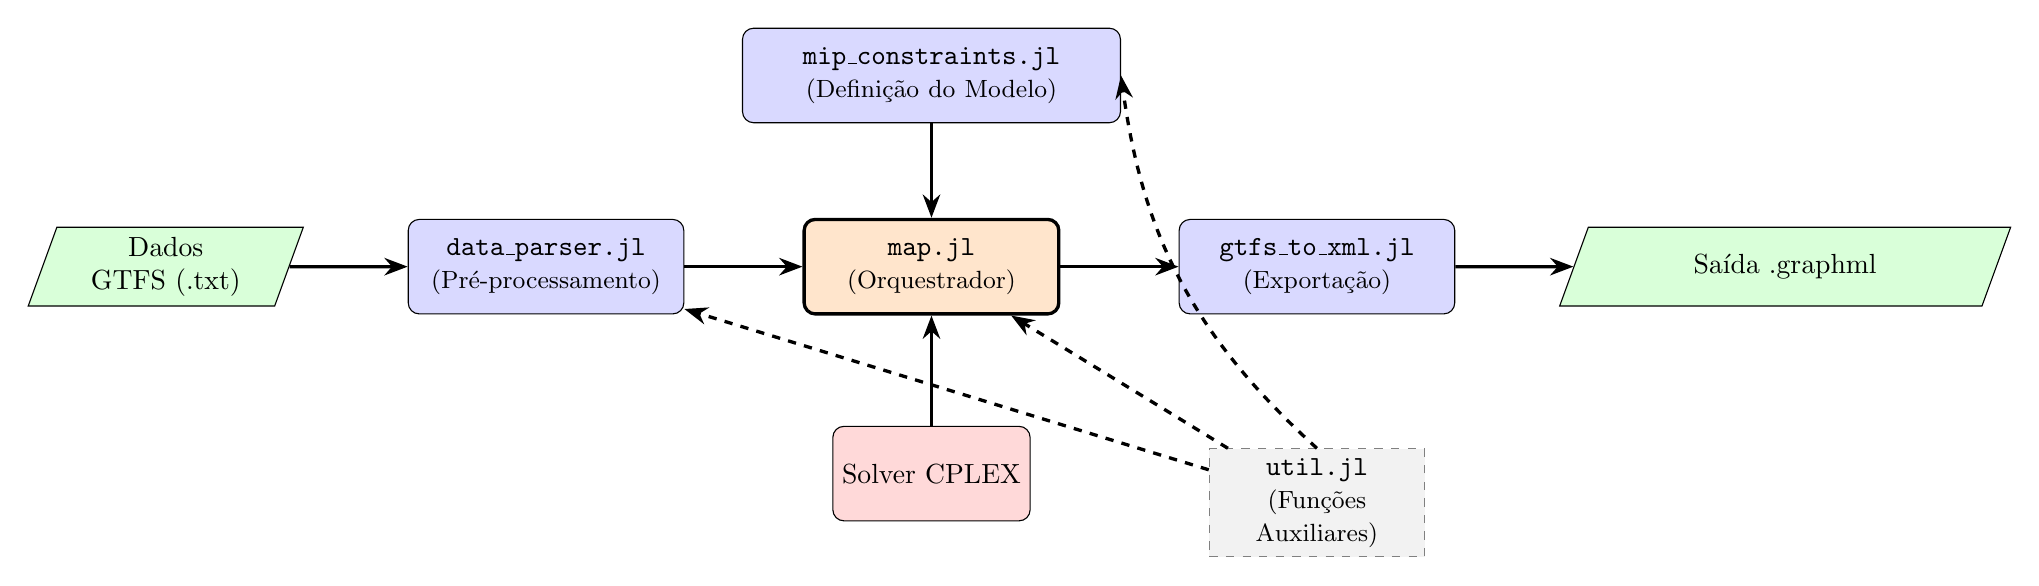
\begin{tikzpicture}[
    node distance=1.2cm and 1.5cm,
    % Estilos dos blocos e setas
    io/.style={trapezium, trapezium left angle=70, trapezium right angle=110, minimum width=2.5cm, minimum height=1cm, text centered, text width=2.5cm, draw=black, fill=green!15},
    modulo/.style={rectangle, rounded corners, minimum width=3.5cm, minimum height=1.2cm, text centered, text width=3cm, draw=black, fill=blue!15},
    modulo_constraint/.style={rectangle, rounded corners, minimum width=4.8cm, minimum height=1.2cm, text centered, text width=4.5cm, draw=black, fill=blue!15},
    modulo_main/.style={rectangle, rounded corners, minimum width=3cm, minimum height=1.2cm, text centered, text width=3cm, draw=black, fill=orange!20, very thick},
    modulo_util/.style={rectangle, dashed, minimum width=2.5cm, minimum height=1cm, text centered, text width=2.5cm, draw=gray, fill=gray!10},
    solver/.style={rectangle, rounded corners, minimum width=2.5cm, minimum height=1.2cm, text centered, draw=black, fill=red!15},
    seta/.style={-Stealth, very thick}
  ]
    % Nós do fluxo principal
    \node (gtfs) [io] {Dados GTFS (.txt)};
    \node (parser) [modulo, right=of gtfs] {\texttt{data\_parser.jl} \\ \small (Pré-processamento)};
    \node (map) [modulo_main, right=of parser] {\texttt{map.jl} \\ \small (Orquestrador)};
    \node (export) [modulo, right=of map] {\texttt{gtfs\_to\_xml.jl} \\ \small (Exportação)};
    \node (graphml) [io, right=of export] {Saída .graphml};

    % Módulos auxiliares
    \node (mip) [modulo_constraint, above=of map] {\texttt{mip\_constraints.jl} \\ \small (Definição do Modelo)};
    \node (cplex) [solver, below=of map, yshift=-0.2cm] {Solver CPLEX};
    \node (utils) [modulo_util, below=of export, yshift=-0.5cm] {\texttt{util.jl} \\ \small (Funções Auxiliares)};

    % Setas do fluxo principal
    \draw[seta] (gtfs) -- (parser); \draw[seta] (parser) -- (map); \draw[seta] (map) -- (export); \draw[seta] (export) -- (graphml);

    % Setas de interação
    \draw[seta] (mip.south) -- (map.north);
    \draw[seta] (cplex.north) to[out=90,in=-90] (map.south);

    % Setas de utilitários (tracejadas)
    \draw[seta, dashed] (utils) -- (parser);
    \draw[seta, dashed] (utils) -- (map);
    \draw[seta, dashed] (utils.north) to[bend left=20] (mip.east);
  \end{tikzpicture}%
  }
\end{figure}


\section{Pré-processamento e Abstração de Dados}
\label{sec:preprocessamento}

A modelagem da rede de transporte coletivo por ônibus de Porto Alegre a partir dos dados no formato GTFS impõe um dilema fundamental referente à topologia do grafo de entrada para o modelo de otimização. Inicialmente, explorou-se a estratégia de construir o grafo a partir das sequências de paradas sucessivas descritas no arquivo \texttt{stops.txt}, preservando integralmente os pontos de embarque e desembarque das rotas — informação essencial para a usabilidade do mapa esquemático. Contudo, a malha gerada por essa abordagem revelou-se excessivamente complexa, mesmo após a aplicação de técnicas de simplificação. O principal obstáculo reside no elevado grau de conectividade de determinados nós: o grafo baseado exclusivamente em paradas apresentou 61 vértices com grau superior a 4, incluindo dois vértices de grau 7 e um vértice de grau 8. Como a discretização octilinear dispõe de apenas oito direções espaciais, levanta-se a hipótese de que vértices com grau superior a 5 possam saturar a capacidade angular das interseções e impor um gargalo de desempenho ao solver MIP, em virtude do crescimento de variáveis binárias e restrições exigidas para governar a ordem circular das arestas incidentes (Equações~\ref{eq:beta_sum} e~\ref{eq:circular_order}).

Por outro lado, a construção do grafo pode ter como base o traçado geométrico real das vias contido no arquivo \texttt{shapes.txt}. Nessa modelagem, os vértices mantêm graus estritamente inferiores a 5, uma vez que o desenho reflete a infraestrutura viária urbana, na qual interseções com mais de cinco vias são extremamente raras. Contudo, a utilização exclusiva dessa malha física implica a perda das informações de embarque e desembarque, descaracterizando o propósito funcional do mapa. Para conciliar ambos os requisitos, desenvolveu-se uma solução híbrida que adota a topologia viária de \texttt{shapes.txt} como grafo estrutural base (\textit{backbone}), acoplando a ela as informações semânticas e operacionais de \texttt{stops.txt}.

Após a estruturação desse grafo híbrido, a rede é submetida a um conjunto de técnicas de simplificação topológica: a aderência de vértices a arestas (\textit{snapping}), o agrupamento de paradas próximas por limiar de distância, e, por fim, a eliminação de vértices intermediários adjacentes. Tais procedimentos visam abstrair a complexidade geométrica da rede e reduzir sua escala computacional, mantendo informações essenciais e a clareza do mapa mental do usuário. Os detalhes da construção do grafo híbrido e os aspectos de cada etapa de simplificação topológica são aprofundados a seguir.

\subsection{Construção do Grafo Híbrido}
\label{subsec:construcao_grafo_hibrido}

A concepção do grafo híbrido inicia-se com a estruturação independente de duas representações topológicas a partir dos dados do GTFS: o grafo de paradas (\textit{stops}) e o grafo de traçados (\textit{shapes}).

Para a construção do grafo de paradas, realiza-se inicialmente a junção relacional entre as tabelas \texttt{stop\_times.txt} e \texttt{trips.txt}, mapeando as viagens. Cada parada registrada em \texttt{stops.txt} é convertida em um vértice contendo sua respectiva coordenada geográfica $(\text{lat}, \text{lon})$ e seu nome textual. As arestas são então estabelecidas iterando-se sobre a sequência de paradas (\texttt{stop\_sequence}) de cada viagem, criando conexões diretas entre paradas consecutivas e registrando nas arestas o conjunto de rotas que realizam aquele trajeto.

Paralelamente, o grafo de traçado físico (\textit{backbone}) é construído a partir do arquivo \texttt{shapes.txt}. Os pontos geográficos (\texttt{shape\_pt\_lat}, \texttt{shape\_pt\_lon}) são ordenados sequencialmente através do campo \texttt{shape\_pt\_sequence} para cada identificador de traçado (\texttt{shape\_id}). Cada coordenada geográfica única é associada a um vértice geométrico no grafo, enquanto pontos consecutivos ao longo do trajeto formam as arestas da malha viária física, as quais herdam a cobertura de todas as linhas de ônibus associadas àquele respectivo \textit{shape}.

Uma análise inicial do grafo de paradas revelou a existência de arestas com comprimentos anômalos, que se estendiam por distâncias significativamente maiores que as demais. A verificação com mapas geográficos das rotas confirmou que tais conexões representavam falhas na modelagem dos dados, e não trechos contínuos de percurso. Diante disso, essas arestas foram removidas, e as lacunas resultantes na topologia da rede foram corrigidas pela inserção manual de conexões apropriadas, restabelecendo a continuidade dos trajetos, como ilustrado na Figura~\ref{fig:anomalia_correcao}.

\begin{figure}[htbp]
    \centering
    \begin{minipage}{0.48\textwidth}
        \centering
        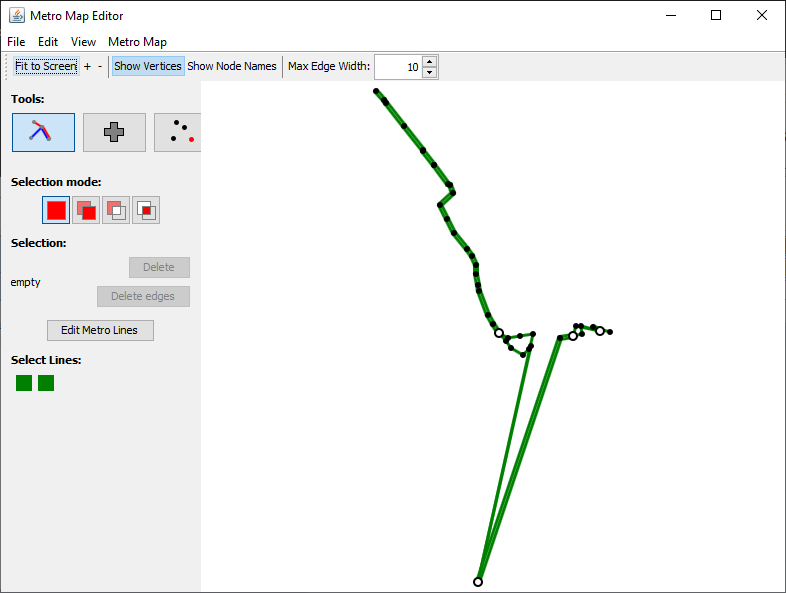
\includegraphics[width=\linewidth, trim=160 2 120 62, clip]{imagens/anomalia_antes.png}
    \end{minipage}\hfill
    \begin{minipage}{0.48\textwidth}
        \centering
        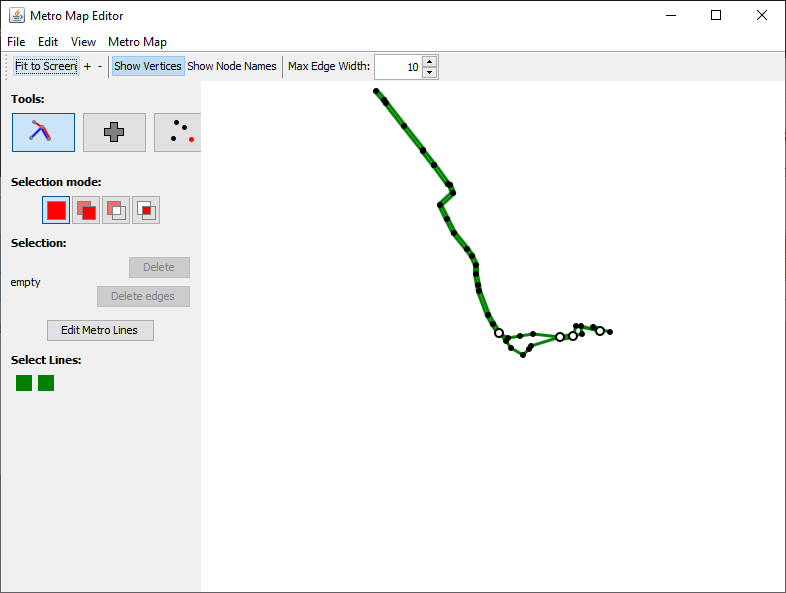
\includegraphics[width=\linewidth, trim=160 2 120 62, clip]{imagens/anomalia_depois.png}
    \end{minipage}
    \caption{Comparação da remoção de anomalias. À esquerda, as arestas com comprimentos anômalos. À direita, a rede após a correção manual.}
    \label{fig:anomalia_correcao}
\end{figure}

O grafo de traçado é então submetido à fusão de vértices e \textit{snapping} de vértices a arestas próximas (cujo detalhamento é apresentado na Seção~\ref{subsec:snapping}), com o objetivo de mitigar redundâncias espaciais decorrentes dos sentidos opostos de circulação em uma mesma via que, de outro modo, produziriam segmentos paralelos artificiais. Ao final dessa etapa preparatória, obtêm-se as duas malhas estruturadas: o grafo de paradas e o grafo de traçado viário. A Figura~\ref{fig:comparativo_grafos_iniciais} ilustra essas duas representações, nas quais os pontos pretos representam vértices adjacentes (de grau~2) e os pontos brancos destacam vértices com grau superior a~2, indicando bifurcações e cruzamentos da rede.

\begin{figure}[H]
    \centering
    \begin{subfigure}[b]{0.48\textwidth}
        \centering
        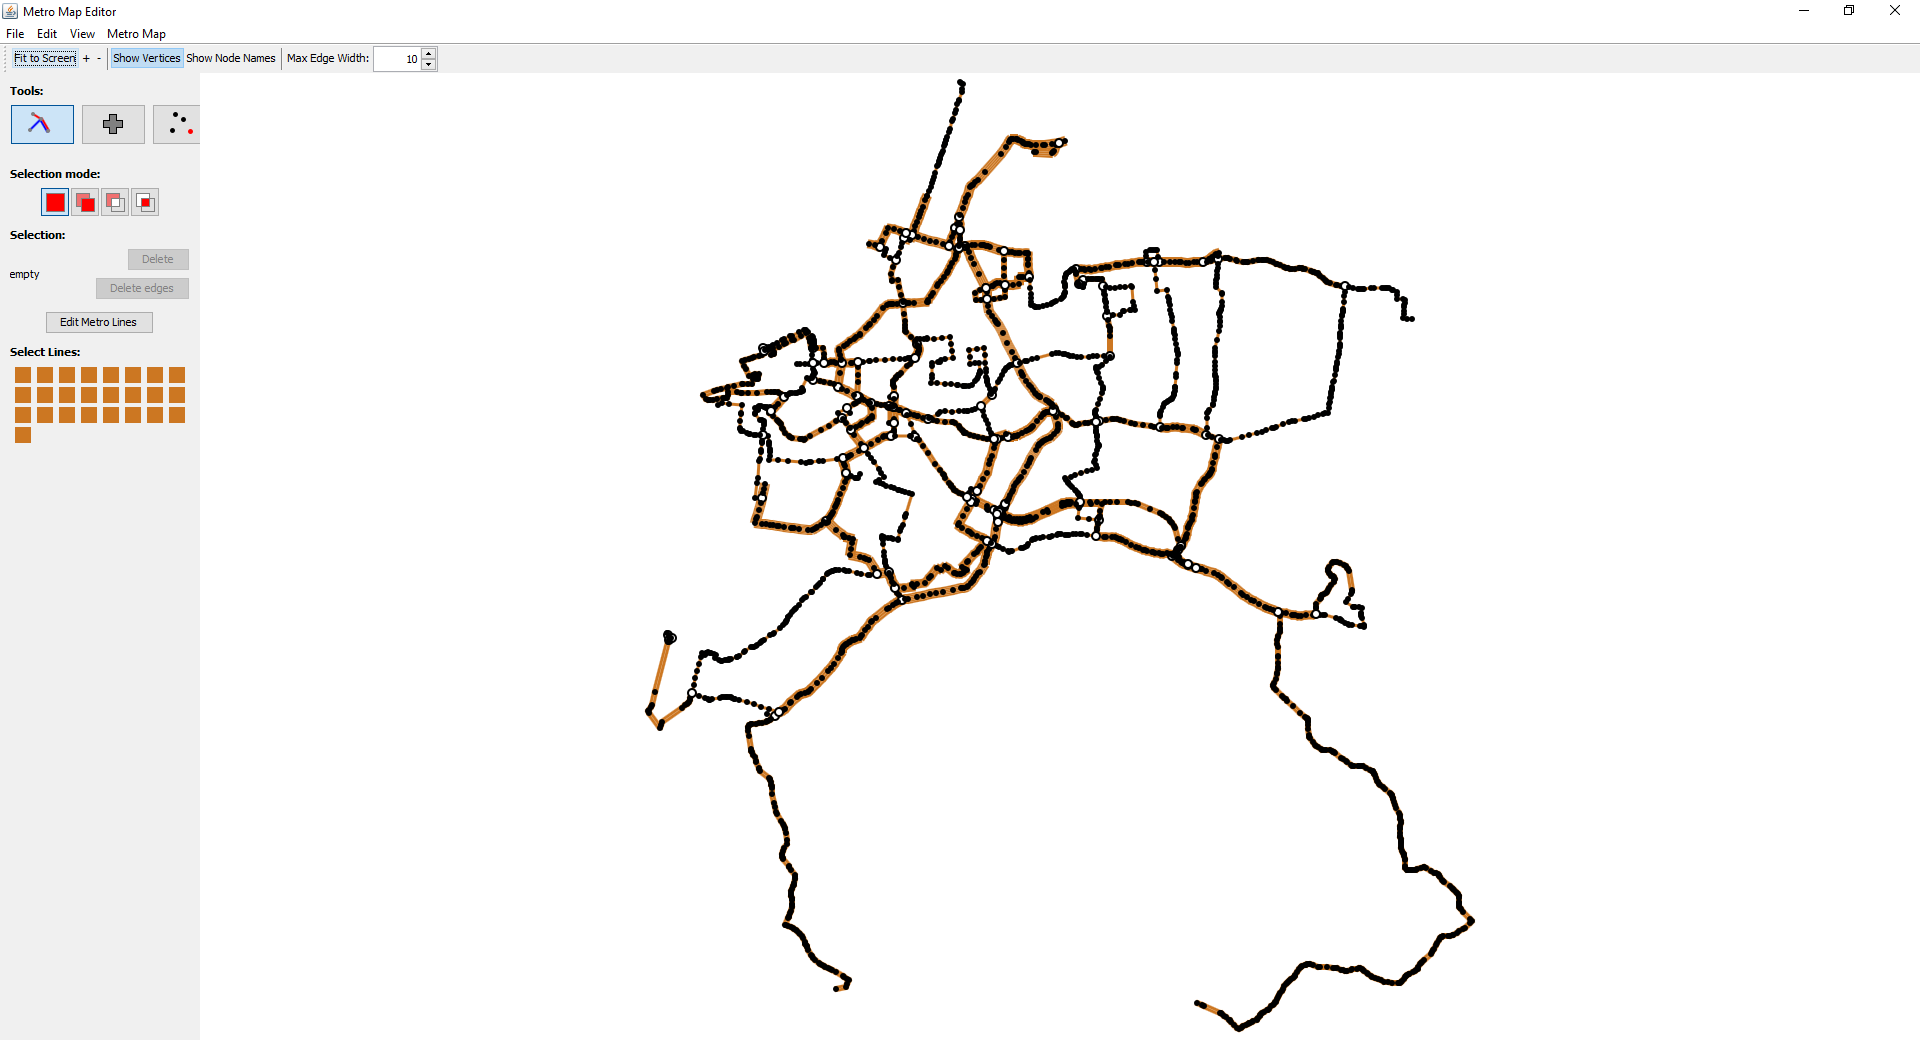
\includegraphics[width=\linewidth, trim=480 0 320 60, clip]{imagens/mapa_tracado.png}
        \caption{Grafo de traçado (\textit{shapes}).}
        \label{fig:grafo_tracado}
    \end{subfigure}
    \hfill
    \begin{subfigure}[b]{0.48\textwidth}
        \centering
        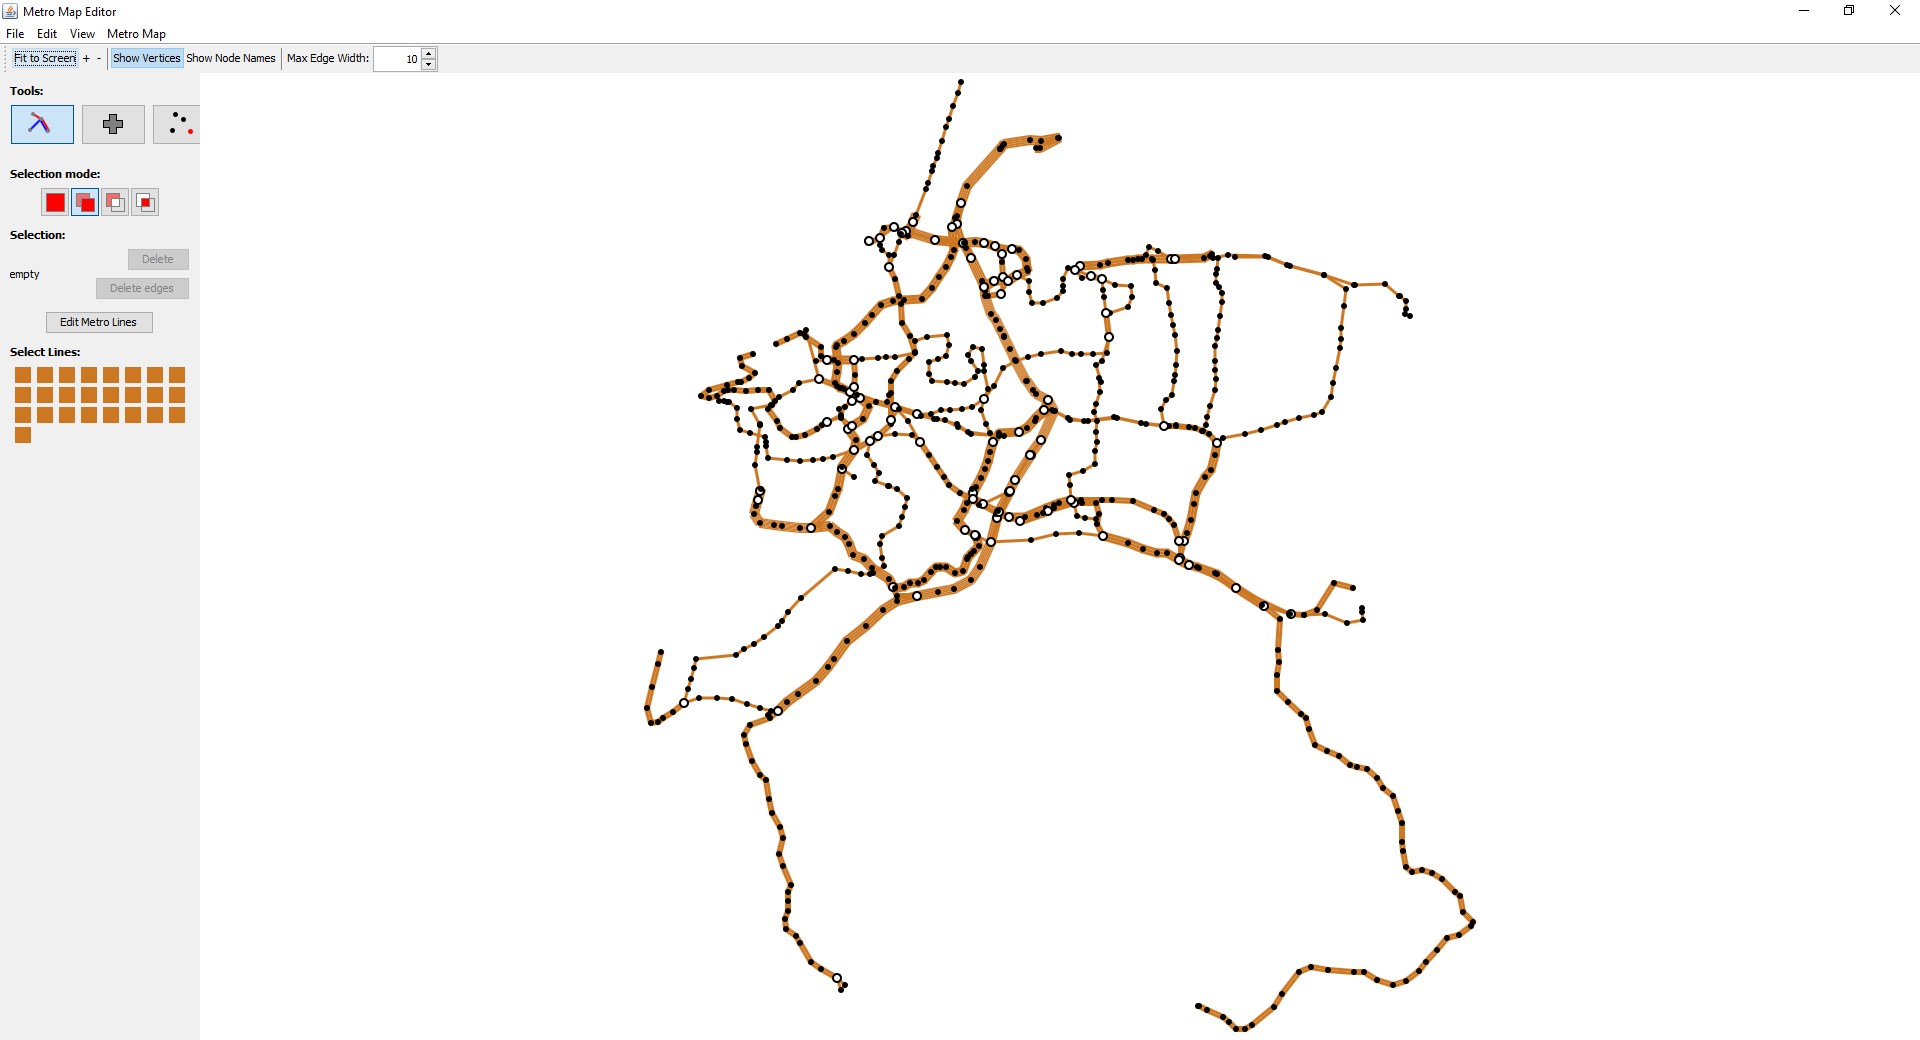
\includegraphics[width=\linewidth, trim=480 0 320 60, clip]{imagens/mapa_paradas.png}
        \caption{Grafo de paradas (\textit{stops}).}
        \label{fig:grafo_paradas}
    \end{subfigure}
    \caption{Comparativo das representações iniciais da rede de transporte: o grafo de traçado físico (a) e o grafo operacional de paradas (b). Os pontos pretos indicam vértices adjacentes, enquanto os pontos brancos representam vértices com grau superior a 2 (bifurcações e cruzamentos).}
    \label{fig:comparativo_grafos_iniciais}
\end{figure}

Com a estruturação de ambas as malhas concluída, inicia-se a etapa de acoplamento das paradas sobre a malha viária física (\textit{backbone}), empregando-se a técnica de projeção geométrica (\textit{snapping}). Contudo, a sobreposição das camadas revelou desafios significativos: embora ambos os grafos apresentem alta similaridade visual global, constataram-se discrepâncias entre as coordenadas geográficas dos dois grafos para um mesmo local físico. A Figura~\ref{fig:compara_tracado_parada} ilustra esse fenômeno na região da Avenida Assis Brasil, evidenciando o descompasso entre o traçado contínuo das vias (em laranja) e o grafo derivado das paradas (em linhas pontilhadas). Em decorrência dessa divergência de georreferenciamento intrínseca aos dados brutos do GTFS, alguns pontos de parada situaram-se a distâncias consideráveis da via correspondente — excedendo, em determinados casos, 100 metros —, o que exigiu tratamentos heurísticos específicos para evitar a aderência incorreta a arestas de vias adjacentes ou paralelas.

Para contornar essa imprecisão, implementou-se uma heurística de priorização semântica por compatibilidade de rotas durante o \textit{snapping}: ao buscar o segmento viário de destino para uma parada, o algoritmo prioriza arestas do traçado que compartilham ao menos uma linha de ônibus atendida por aquele ponto, mesmo que existam outras arestas espacialmente mais próximas pertencentes a outras linhas. Caso nenhuma aresta com rotas coincidentes seja identificada dentro do limiar de busca, adota-se uma estratégia de contingência (\textit{fallback}), associando a parada à aresta viária geometricamente mais próxima. Esse mecanismo reduz as associações indevidas e eleva a fidelidade dos itinerários vinculados às vias correspondentes, cujos ganhos percentuais são avaliados quantitativamente na Seção~\ref{sec:analise_quantitativa}.

\begin{figure}[H]
    \centering
    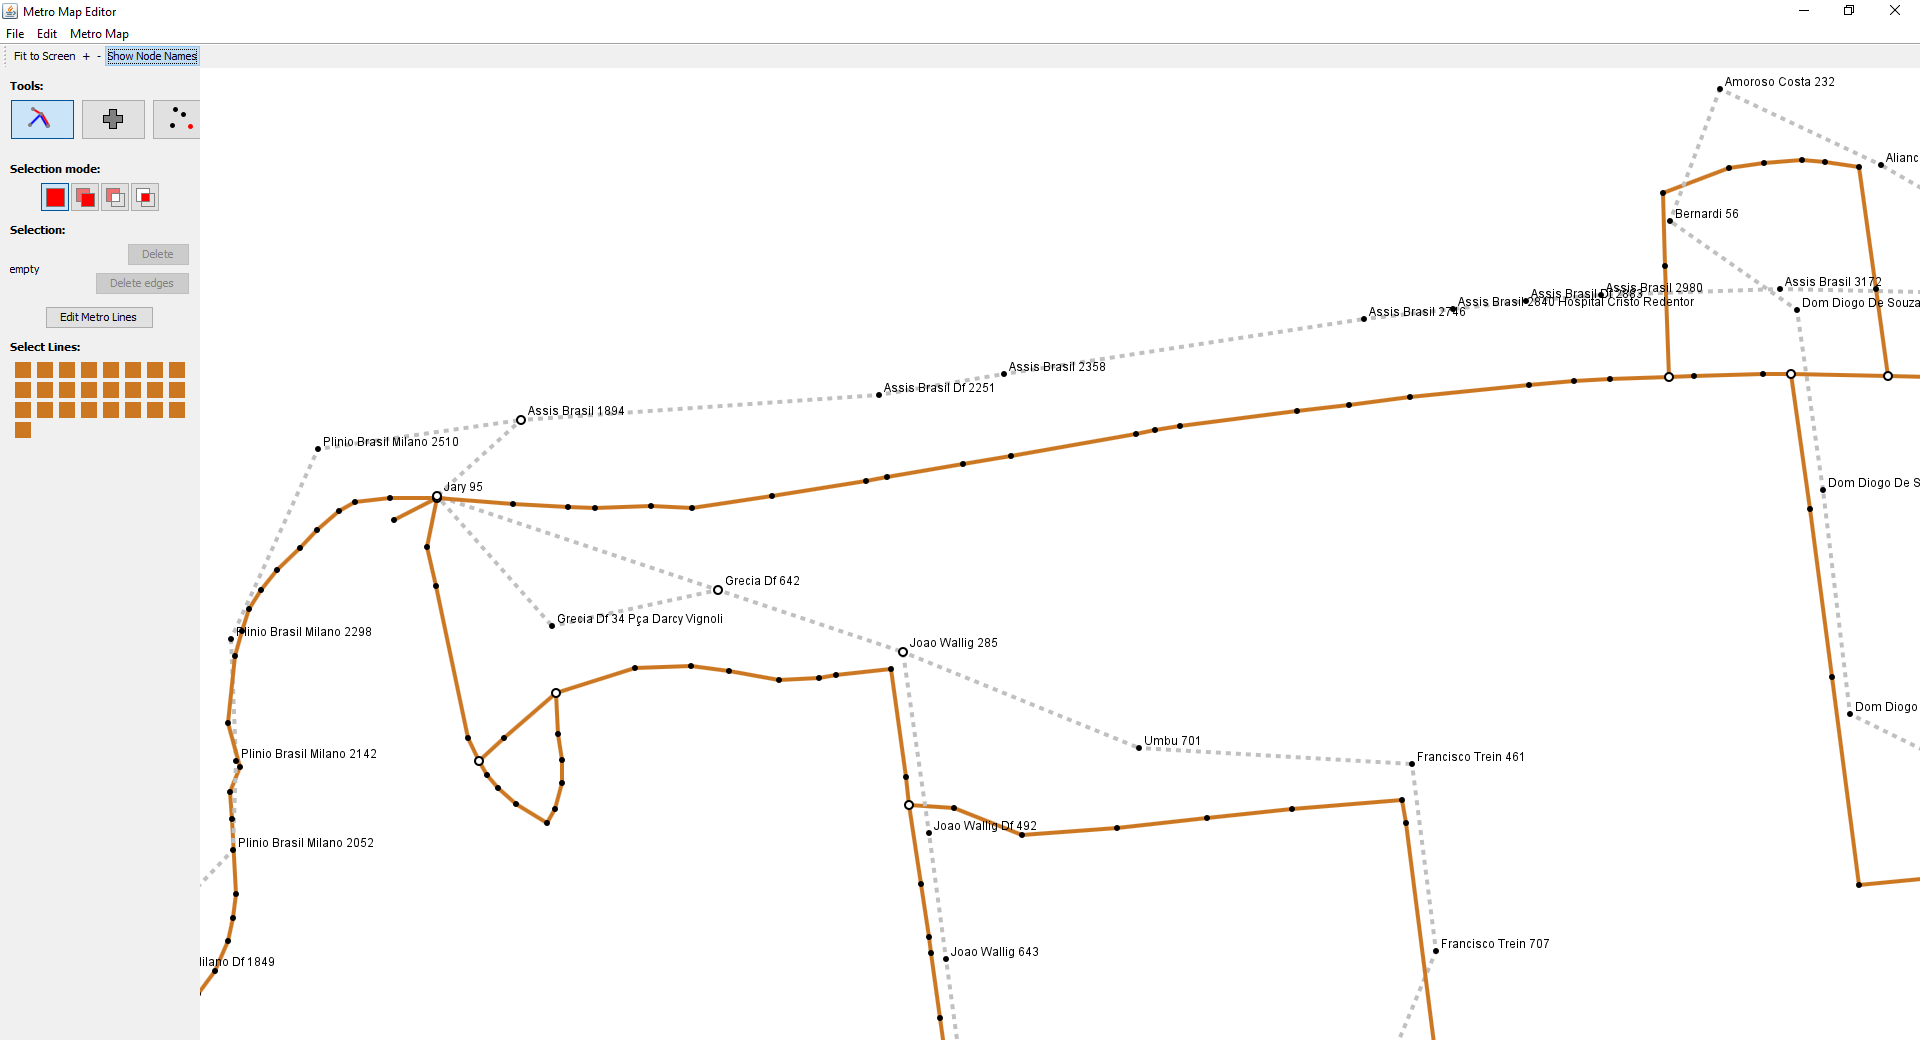
\includegraphics[width=0.85\linewidth, trim=160 0 160 60, clip]{imagens/mapa_compara_tracado_parada.png}
    \caption{Comparação e sobreposição espacial dos dois grafos na região da Avenida Assis Brasil: o grafo de traçado físico (\textit{shapes}, em linha sólida laranja) e o grafo operacional de conexões entre paradas (\textit{stops}, em linhas pontilhadas).}
    \label{fig:compara_tracado_parada}
\end{figure}

Concluída a projeção geométrica descrita, obtém-se uma malha integrada contendo tanto os vértices correspondentes às paradas quanto os pontos intermediários herdados do traçado físico de \texttt{shapes.txt}. A etapa subsequente consiste em uma contração topológica do grafo, eliminando os nós intermediários do \textit{backbone} que não agregam valor estrutural à rede — isto é, vértices que não correspondem a paradas e possuem grau de conectividade estritamente igual a 2. Esse procedimento remove os nós colineares redundantes e conecta diretamente suas extremidades adjacentes, preservando o conjunto de rotas associadas. Como resultado, ilustrado na Figura~\ref{fig:contracao_shape_nodes}, o grafo passa a ser constituído exclusivamente por vértices de paradas e por nós estruturais que representam cruzamentos e bifurcações viárias. Esta contração constitui a etapa final de consolidação do grafo híbrido, resultando na malha unificada que servirá de base para as etapas posteriores de abstração e simplificação da rede.


\begin{figure}[H]
    \centering
    % --- ANTES DA CONTRAÇÃO ---
    \begin{subfigure}[b]{0.48\textwidth}
        \centering
        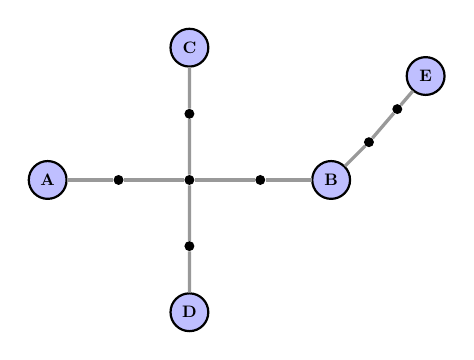
\begin{tikzpicture}[
            scale=0.6,
            every node/.style={transform shape},
            stop_node/.style={circle, draw=black, fill=blue!25, thick, minimum size=0.8cm, font=\bfseries},
            shape_node/.style={circle, fill=black, inner sep=0pt, minimum size=6pt},
            edge_style/.style={very thick, gray!80}
        ]
            % Paradas principais
            \node[stop_node] (A) at (0, 0) {A};
            \node[stop_node] (B) at (6, 0) {B};
            \node[stop_node] (C) at (3, 2.8) {C};
            \node[stop_node] (D) at (3, -2.8) {D};
            \node[stop_node] (E) at (8, 2.2) {E};

            % Nós intermediários (pontos pretos)
            \node[shape_node] (s1) at (1.5, 0) {};
            \node[shape_node] (cross) at (3, 0) {};
            \node[shape_node] (s2) at (4.5, 0) {};
            
            \node[shape_node] (s3) at (3, 1.4) {};
            \node[shape_node] (s4) at (3, -1.4) {};
            
            \node[shape_node] (s5) at (6.8, 0.8) {};
            \node[shape_node] (s6) at (7.4, 1.5) {};

            % Arestas
            \draw[edge_style] (A) -- (s1) -- (cross) -- (s2) -- (B);
            \draw[edge_style] (C) -- (s3) -- (cross) -- (s4) -- (D);
            \draw[edge_style] (B) -- (s5) -- (s6) -- (E);
        \end{tikzpicture}
        \caption{Antes da contração.}
        \label{fig:contracao_antes}
    \end{subfigure}
    \hfill
    % --- DEPOIS DA CONTRAÇÃO ---
    \begin{subfigure}[b]{0.48\textwidth}
        \centering
        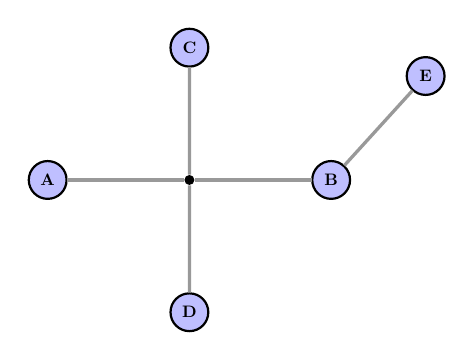
\begin{tikzpicture}[
            scale=0.6,
            every node/.style={transform shape},
            stop_node/.style={circle, draw=black, fill=blue!25, thick, minimum size=0.8cm, font=\bfseries},
            shape_node/.style={circle, fill=black, inner sep=0pt, minimum size=6pt},
            edge_style/.style={very thick, gray!80}
        ]
            % Paradas principais
            \node[stop_node] (A) at (0, 0) {A};
            \node[stop_node] (B) at (6, 0) {B};
            \node[stop_node] (C) at (3, 2.8) {C};
            \node[stop_node] (D) at (3, -2.8) {D};
            \node[stop_node] (E) at (8, 2.2) {E};

            % Apenas o nó de cruzamento (grau 4) é preservado
            \node[shape_node] (cross) at (3, 0) {};

            % Arestas reconectadas diretamente
            \draw[edge_style] (A) -- (cross);
            \draw[edge_style] (cross) -- (B);
            \draw[edge_style] (C) -- (cross);
            \draw[edge_style] (cross) -- (D);
            \draw[edge_style] (B) -- (E);
        \end{tikzpicture}
        \caption{Após a contração.}
        \label{fig:contracao_depois}
    \end{subfigure}
    \caption{Processo de contração de nós do traçado: (a) grafo integrado contendo nós intermediários de grau 2 e o cruzamento viário; (b) grafo simplificado após a eliminação dos pontos colineares de grau 2, preservando os cruzamentos estruturais e as paradas de embarque.}
    \label{fig:contracao_shape_nodes}
\end{figure}

A fim de avaliar quantitativamente a fidelidade topológica do Grafo Híbrido, foi desenvolvida uma rotina que opera mediante a extração e a comparação dos conjuntos de paradas por rota:

\begin{enumerate}
    \item Para cada rota $r \in \mathcal{R}$ do sistema, extrai-se o conjunto $\mathcal{S}_{\text{stops}}(r)$ contendo as paradas originalmente vinculadas à rota no grafo bruto de paradas ($G_{\text{stops}}$);
    \item De forma análoga, extrai-se o conjunto $\mathcal{S}_{\text{híbrido}}(r)$, correspondente às paradas retidas e associadas à rota $r$ na estrutura do grafo híbrido unificado ($G_{\text{híbrido}}$);
    \item Determina-se a quantidade de paradas omitidas na rota $r$ como $m(r) = |\mathcal{S}_{\text{stops}}(r) \setminus \mathcal{S}_{\text{híbrido}}(r)|$, computando-se a taxa global de retenção de paradas ($\tau_{\text{ret}}$) expressa na Equação~\ref{eq:taxa_retencao_paradas}:
\end{enumerate}

\begin{equation}
\tau_{\text{ret}} = \frac{\sum_{r \in \mathcal{R}} |\mathcal{S}_{\text{stops}}(r) \cap \mathcal{S}_{\text{híbrido}}(r)|}{\sum_{r \in \mathcal{R}} |\mathcal{S}_{\text{stops}}(r)|} = 1 - \frac{\sum_{r \in \mathcal{R}} m(r)}{\sum_{r \in \mathcal{R}} |\mathcal{S}_{\text{stops}}(r)|}.
\label{eq:taxa_retencao_paradas}
\end{equation}

A Figura~\ref{fig:fluxo_grafo_hibrido} ilustra esquematicamente esse processo de projeção geométrica e validação, cujos resultados quantitativos são avaliados na Seção~\ref{subsec:analise_grafo_hibrido}.

\begin{figure}[H]
    \centering
    \resizebox{\textwidth}{!}{%
    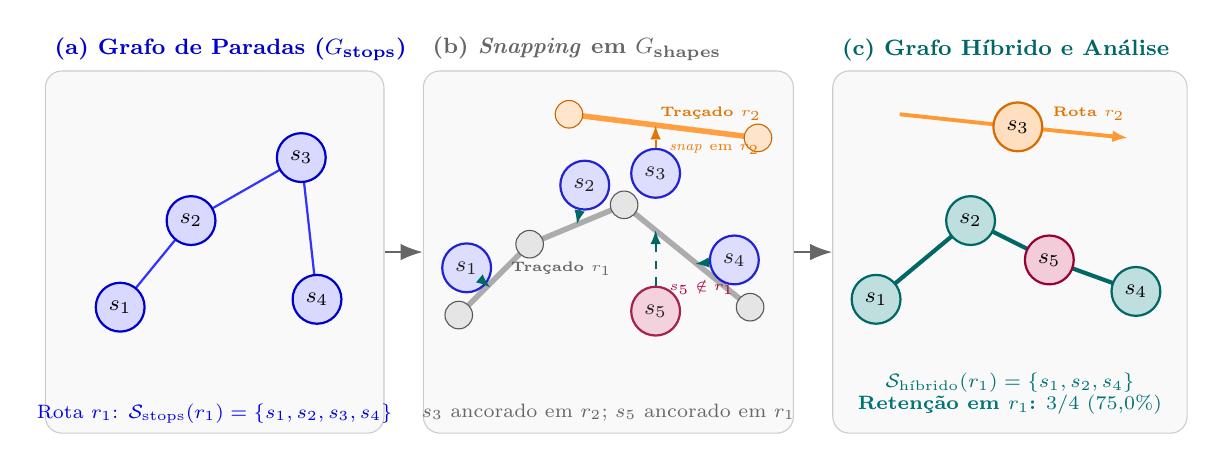
\begin{tikzpicture}[
        stop_node/.style={circle, draw=blue!80!black, thick, fill=blue!15, minimum size=0.62cm, inner sep=0pt, font=\bfseries\footnotesize},
        shape_node/.style={circle, draw=gray!70!black, fill=gray!20, minimum size=0.35cm, inner sep=0pt},
        hybrid_node/.style={circle, draw=teal!80!black, thick, fill=teal!25, minimum size=0.62cm, inner sep=0pt, font=\bfseries\footnotesize},
        other_route_node/.style={circle, draw=orange!85!black, thick, fill=orange!25, minimum size=0.62cm, inner sep=0pt, font=\bfseries\footnotesize},
        ext_node/.style={circle, draw=purple!80!black, thick, fill=purple!20, minimum size=0.62cm, inner sep=0pt, font=\bfseries\footnotesize},
        box_panel/.style={draw=gray!40, fill=gray!5, rounded corners=6pt, inner sep=7pt},
        arrow_flow/.style={-{Latex[length=2.8mm]}, thick, gray!80!black}
    ]
        % --- PAINEL A: Grafo de Paradas Original ---
        \node[box_panel, minimum width=4.3cm, minimum height=4.6cm] (panelA) at (0, 0) {};
        \node[above right, font=\bfseries\footnotesize, text=blue!80!black] at (panelA.north west) {(a) Grafo de Paradas ($G_{\text{stops}}$)};
        
        \coordinate (S1) at (-1.2, -0.7);
        \coordinate (S2) at (-0.3, 0.4);
        \coordinate (S3) at (1.1, 1.2);
        \coordinate (S4) at (1.3, -0.6);
        
        \draw[thick, blue!80, -{Latex[length=2.2mm]}] (S1) -- (S2);
        \draw[thick, blue!80, -{Latex[length=2.2mm]}] (S2) -- (S3);
        \draw[thick, blue!80, -{Latex[length=2.2mm]}] (S3) -- (S4);
        
        \node[stop_node] at (S1) {$s_1$};
        \node[stop_node] at (S2) {$s_2$};
        \node[stop_node] at (S3) {$s_3$};
        \node[stop_node] at (S4) {$s_4$};
        \node[below, font=\scriptsize, text=blue!90!black] at (0, -1.8) {Rota $r_1$: $\mathcal{S}_{\text{stops}}(r_1) = \{s_1, s_2, s_3, s_4\}$};

        % --- PAINEL B: Grafo de Shapes e Snapping ---
        \node[box_panel, minimum width=4.7cm, minimum height=4.6cm] (panelB) at (5.0, 0) {};
        \node[above right, font=\bfseries\footnotesize, text=gray!80!black] at (panelB.north west) {(b) \textit{Snapping} em $G_{\text{shapes}}$};
        
        % Linha de shape contínua (Rota r1)
        \coordinate (W1) at (3.1, -0.8);
        \coordinate (W2) at (4.0, 0.1);
        \coordinate (W3) at (5.2, 0.6);
        \coordinate (W4) at (6.8, -0.7);
        
        \draw[line width=2pt, gray!65] (W1) -- (W2) -- (W3) -- (W4);
        \node[shape_node] at (W1) {};
        \node[shape_node] at (W2) {};
        \node[shape_node] at (W3) {};
        \node[shape_node] at (W4) {};
        \node[font=\tiny\bfseries, text=gray!80!black, below] at (4.4, 0.0) {Traçado $r_1$};

        % Linha de shape de outra rota (Rota r2 / via adjacente mais ao alto)
        \coordinate (R2_A) at (4.5, 1.75);
        \coordinate (R2_B) at (6.9, 1.45);
        \draw[line width=2pt, orange!75] (R2_A) -- (R2_B);
        \node[shape_node, draw=orange!80!black, fill=orange!20] at (R2_A) {};
        \node[shape_node, draw=orange!80!black, fill=orange!20] at (R2_B) {};
        \node[font=\tiny\bfseries, text=orange!90!black, above] at (6.3, 1.55) {Traçado $r_2$};

        % Paradas originais
        \node[stop_node, opacity=0.85] (p1_orig) at (3.2, -0.2) {$s_1$};
        \node[stop_node, opacity=0.85] (p2_orig) at (4.7, 0.85) {$s_2$};
        \node[stop_node, opacity=0.85] (p3_orig) at (5.6, 1.0) {$s_3$};
        \node[stop_node, opacity=0.85] (p4_orig) at (6.6, -0.1) {$s_4$};
        % Parada externa s5 (não pertencente a r1)
        \node[ext_node, opacity=0.85] (p5_orig) at (5.6, -0.75) {$s_5$};

        % Projeções ortogonais corretas (em r1)
        \draw[dashed, thick, teal!80!black, -{Latex[length=1.8mm]}] (p1_orig) -- (3.5, -0.45);
        \draw[dashed, thick, teal!80!black, -{Latex[length=1.8mm]}] (p2_orig) -- (4.6, 0.35);
        \draw[dashed, thick, teal!80!black, -{Latex[length=1.8mm]}] (p4_orig) -- (6.1, -0.15);

        % Projeção incorreta de s3 para a aresta de r2 (para cima)
        \draw[dashed, thick, orange!90!black, -{Latex[length=1.8mm]}] (p3_orig) -- (5.6, 1.61);
        \node[font=\tiny, text=orange!95!black, right] at (5.65, 1.3) {\textit{snap} em $r_2$};

        % Projeção de s5 para a aresta de r1 (para cima)
        \draw[dashed, thick, teal!80!black, -{Latex[length=1.8mm]}] (p5_orig) -- (5.6, 0.28);
        \node[font=\tiny, text=purple!90!black, right] at (5.65, -0.45) {$s_5 \notin r_1$};
        
        \node[below, font=\scriptsize, text=gray!80!black] at (5.0, -1.8) {$s_3$ ancorado em $r_2$; $s_5$ ancorado em $r_1$};

        % --- PAINEL C: Grafo Híbrido Final ---
        \node[box_panel, minimum width=4.5cm, minimum height=4.6cm] (panelC) at (10.1, 0) {};
        \node[above right, font=\bfseries\footnotesize, text=teal!80!black] at (panelC.north west) {(c) Grafo Híbrido e Análise};
        
        % Aresta da rota r2 com s3 incorporado
        \coordinate (HR2_A) at (8.7, 1.75);
        \coordinate (HR2_B) at (11.6, 1.45);
        \coordinate (H3) at (10.2, 1.59);
        \draw[line width=1.4pt, orange!80, -{Latex[length=2.0mm]}] (HR2_A) -- (H3);
        \draw[line width=1.4pt, orange!80, -{Latex[length=2.0mm]}] (H3) -- (HR2_B);
        \node[other_route_node] at (H3) {$s_3$};
        \node[font=\tiny\bfseries, text=orange!90!black, above] at (11.1, 1.55) {Rota $r_2$};

        % Rota r1 no grafo híbrido (com nós elevados para afastar do subtexto)
        \coordinate (H1) at (8.4, -0.6);
        \coordinate (H2) at (9.6, 0.4);
        \coordinate (H5) at (10.6, -0.1);
        \coordinate (H4) at (11.7, -0.5);
        
        \draw[line width=1.5pt, teal!80!black, -{Latex[length=2.2mm]}] (H1) -- (H2);
        \draw[line width=1.5pt, teal!80!black, -{Latex[length=2.2mm]}] (H2) -- (H5);
        \draw[line width=1.5pt, teal!80!black, -{Latex[length=2.2mm]}] (H5) -- (H4);
        
        \node[hybrid_node] at (H1) {$s_1$};
        \node[hybrid_node] at (H2) {$s_2$};
        \node[ext_node] at (H5) {$s_5$};
        \node[hybrid_node] at (H4) {$s_4$};
        
        \node[align=center, font=\scriptsize, text=teal!90!black] at (10.1, -1.8) {
            $\mathcal{S}_{\text{híbrido}}(r_1) = \{s_1, s_2, s_4\}$ \\
            \textbf{Retenção em $r_1$:} $3/4$ ($75{,}0\%$)
        };

        % Setas entre painéis
        \draw[arrow_flow] (panelA.east) -- (panelB.west);
        \draw[arrow_flow] (panelB.east) -- (panelC.west);

    \end{tikzpicture}%
    }
    \caption{Representação esquemática do procedimento de construção e avaliação do Grafo Híbrido. Em (a), extrai-se a sequência original de paradas da rota $r_1$; em (b), as paradas são projetadas ortogonalmente sobre o traçado viário contínuo, onde $s_3$ sofre \textit{snapping} na aresta de uma via adjacente pertencente à rota $r_2$, enquanto a parada $s_5$ (não pertencente a $r_1$) é ancorada no traçado físico de $r_1$; em (c), obtém-se o grafo híbrido resultante, no qual $s_5$ não afeta a estatística de fidelidade topológica de $r_1$ por não pertencer a rota.}
    \label{fig:fluxo_grafo_hibrido}
\end{figure}

\subsection{Fusão de Paradas}
\label{subsec:snapping}

Após a formação do grafo híbrido, uma análise visual e estatística sobre o grau de conexão dos vértices apresentou uma distribuição topológica densa e fragmentada em determinados pontos, característica da escala microscópica das paradas de ônibus urbanas. Vértices geograficamente próximos e perceptivamente em uma mesma via geram redundâncias espaciais e ampliam o espaço de busca do modelo de otimização. Para reduzir essa complexidade sem descaracterizar as rotas, implementaram-se técnicas de simplificação baseadas na fusão e agrupamento de vértices. A seguir, detalham-se os mecanismos de aderência de paradas a arestas (\textit{snapping}) e a união de paradas com base em limiares de distância.

Primeiramente, paradas que estão muito próximas a arestas foram aderidas a elas, em um processo conhecido como \textit{snapping}, ilustrado na Figura~\ref{fig:snapping_ilustracao}. Para isso, calcula-se a distância de cada parada (ponto $P$) a cada trecho de rota (segmento de reta entre os vértices $U$ e $V$). Este cálculo é realizado projetando-se as coordenadas geográficas em um plano cartesiano local com origem em $U$, onde se determina o parâmetro escalar de projeção $t$ por meio da Equação~\ref{eq:snapping_t}.

\begin{equation}
t = \frac{\vec{UP} \cdot \vec{UV}}{\|\vec{UV}\|^2}.
\label{eq:snapping_t}
\end{equation}

O valor de $t$ define a posição relativa da projeção ortogonal ao longo do segmento. Caso $0 < t < 1$, a projeção recai estritamente no interior da aresta, e a menor distância euclidiana $d$ entre o ponto $P$ e a projeção ortogonal $P'$ é calculada conforme a Equação~\ref{eq:snapping_dist}.

\begin{equation}
d = \|P - (U + t \cdot \vec{UV})\|.
\label{eq:snapping_dist}
\end{equation}

Se essa distância for inferior a um limiar pré-estabelecido ($D_{\text{snap}}$), a aresta original $(U,V)$ é substituída por duas novas arestas, $(U,P)$ e $(P,V)$, efetivamente inserindo a parada no trajeto.

\begin{figure}[H]
    \centering
    \vspace{0.5cm}
    % --- ANTES ---
    \begin{minipage}{0.48\textwidth}
        \centering
        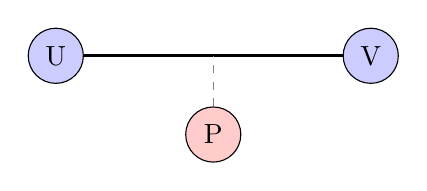
\begin{tikzpicture}[
            node_style/.style={circle, draw, fill=blue!20, minimum size=0.7cm, text centered},
            edge_style/.style={very thick}
        ]
            % Nós
            \node[node_style] (U) at (0,3) {U};
            \node[node_style] (V) at (4,3) {V};
            \node[node_style, fill=red!20] (P) at (2,2) {P};
            
            % Aresta original
            \draw[edge_style] (U) -- (V);
            
            % Linha de projeção
            \draw[dashed, gray] (P) -- (2,3);
        \end{tikzpicture}
    \end{minipage}\hfill
    % --- DEPOIS ---
    \begin{minipage}{0.48\textwidth}
        \centering
        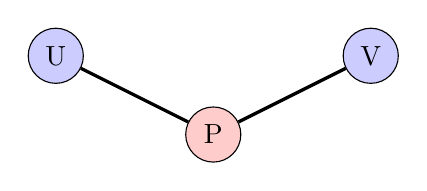
\begin{tikzpicture}[
            node_style/.style={circle, draw, fill=blue!20, minimum size=0.7cm, text centered},
            edge_style/.style={very thick}
        ]
            % Nós
            \node[node_style] (U) at (0,3) {U};
            \node[node_style] (V) at (4,3) {V};
            \node[node_style, fill=red!20] (P) at (2,2) {P}; % P foi movido
            
            % Novas arestas
            \draw[edge_style] (U) -- (P);
            \draw[edge_style] (P) -- (V);
        \end{tikzpicture}
    \end{minipage}
    \vspace{0.5cm}
    \caption{Ilustração do processo de \textit{snapping} de uma parada a uma aresta.}
    \label{fig:snapping_ilustracao}
\end{figure}

Uma segunda estratégia de simplificação adotada consiste na fusão de paradas próximas. Com base na distância euclidiana, paradas com proximidade inferior a um limiar $D_{\text{merge}}$ são unidas em um único vértice, o qual herda as conexões de ambas. A Figura~\ref{fig:fusao_paradas_logica} ilustra essa lógica, mostrando como um vértice principal (P) pode atrair outro vértice (U) dependendo de sua distância.

\begin{figure}[H]
    \centering
    \vspace{0.5cm}
    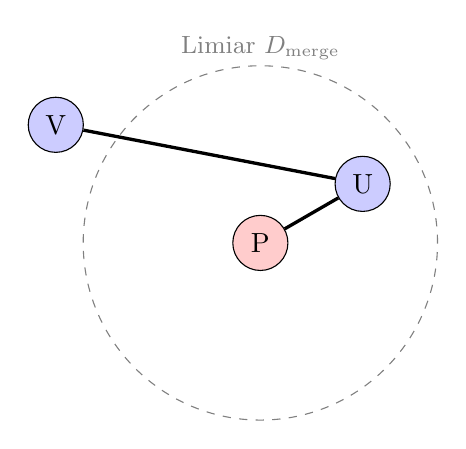
\begin{tikzpicture}[
        node_style/.style={circle, draw, fill=blue!20, minimum size=0.7cm, text centered},
        aura/.style={circle, draw, dashed, gray},
        edge_style/.style={very thick}
    ]
        % Nó principal
        \node[node_style, fill=red!20] (P1) at (0,0) {P};

        % Auras/Limiares de distância
        \node[aura, minimum size=4.5cm] {};
        \node[text=gray, font=\small] at (0,2.2cm) [above] {Limiar $D_{\text{merge}}$};

        % Outros nós para comparação
        \node[node_style] (P2) at (30:1.5cm) {U};
        \node[node_style] (P3) at (150:3cm) {V};

        \draw[edge_style] (P1) -- (P2);
        \draw[edge_style] (P2) -- (P3);
    \end{tikzpicture}
    \caption{Ilustração da lógica de fusão de paradas com limiar de distância.}
    \label{fig:fusao_paradas_logica}
\end{figure}

Para evidenciar o impacto prático dessas estratégias, a Figura~\ref{fig:fusao_pratica} ilustra a simplificação topológica alcançada em um trecho viário na região ao norte do Aeroporto Internacional Salgado Filho. Nota-se que o traçado original, excessivamente entrelaçado, foi substancialmente desobstruído por meio da redução do grau de conectividade de múltiplos nós; essa regularização não apenas aprimora a legibilidade visual das rotas, como também reduz consideravelmente a complexidade imposta à resolução do modelo matemático. A definição dos limiares de distância adotados para o \textit{snapping} e para a união de paradas resultou de uma calibração empírica sistemática, na qual diferentes combinações de valores foram avaliadas quanto à redução da complexidade topológica do grafo. O critério que conduziu essa escolha baseou-se na distribuição dos graus de conectividade dos nós, priorizando configurações que eliminassem vértices de grau crítico ($\deg(v) > 4$). Uma análise quantitativa aprofundada desses parâmetros e dos impactos das distâncias sobre o grau máximo do grafo é apresentada na Seção~\ref{sec:analise_quantitativa}.

\begin{figure}[H]
    \centering
    \vspace{0.5cm}
    % --- ANTES ---
    \begin{minipage}{0.48\textwidth}
        \centering
        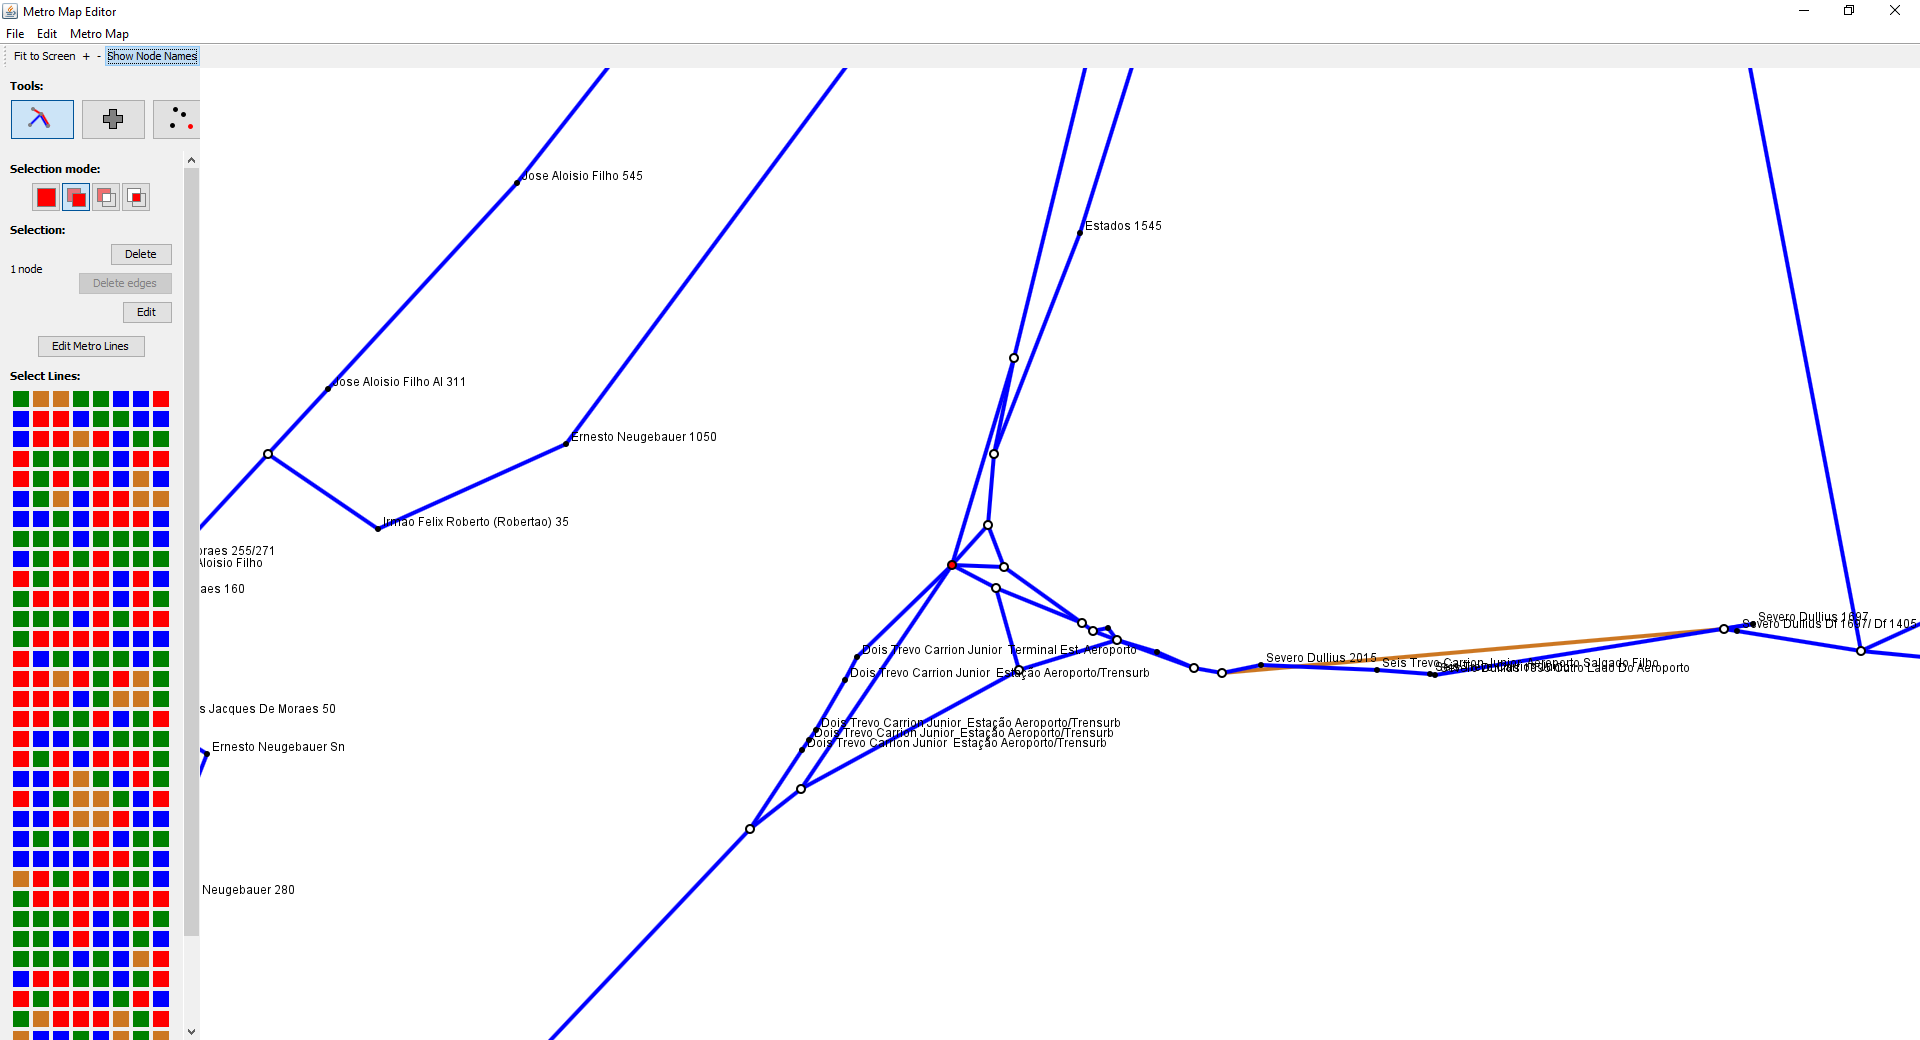
\includegraphics[width=\linewidth, trim=558 100 560 160, clip]{imagens/abstracao_antes.png}
        \subcaption{Antes da fusão.}
    \end{minipage}\hfill
    % --- DEPOIS ---
    \begin{minipage}{0.48\textwidth}
        \centering
        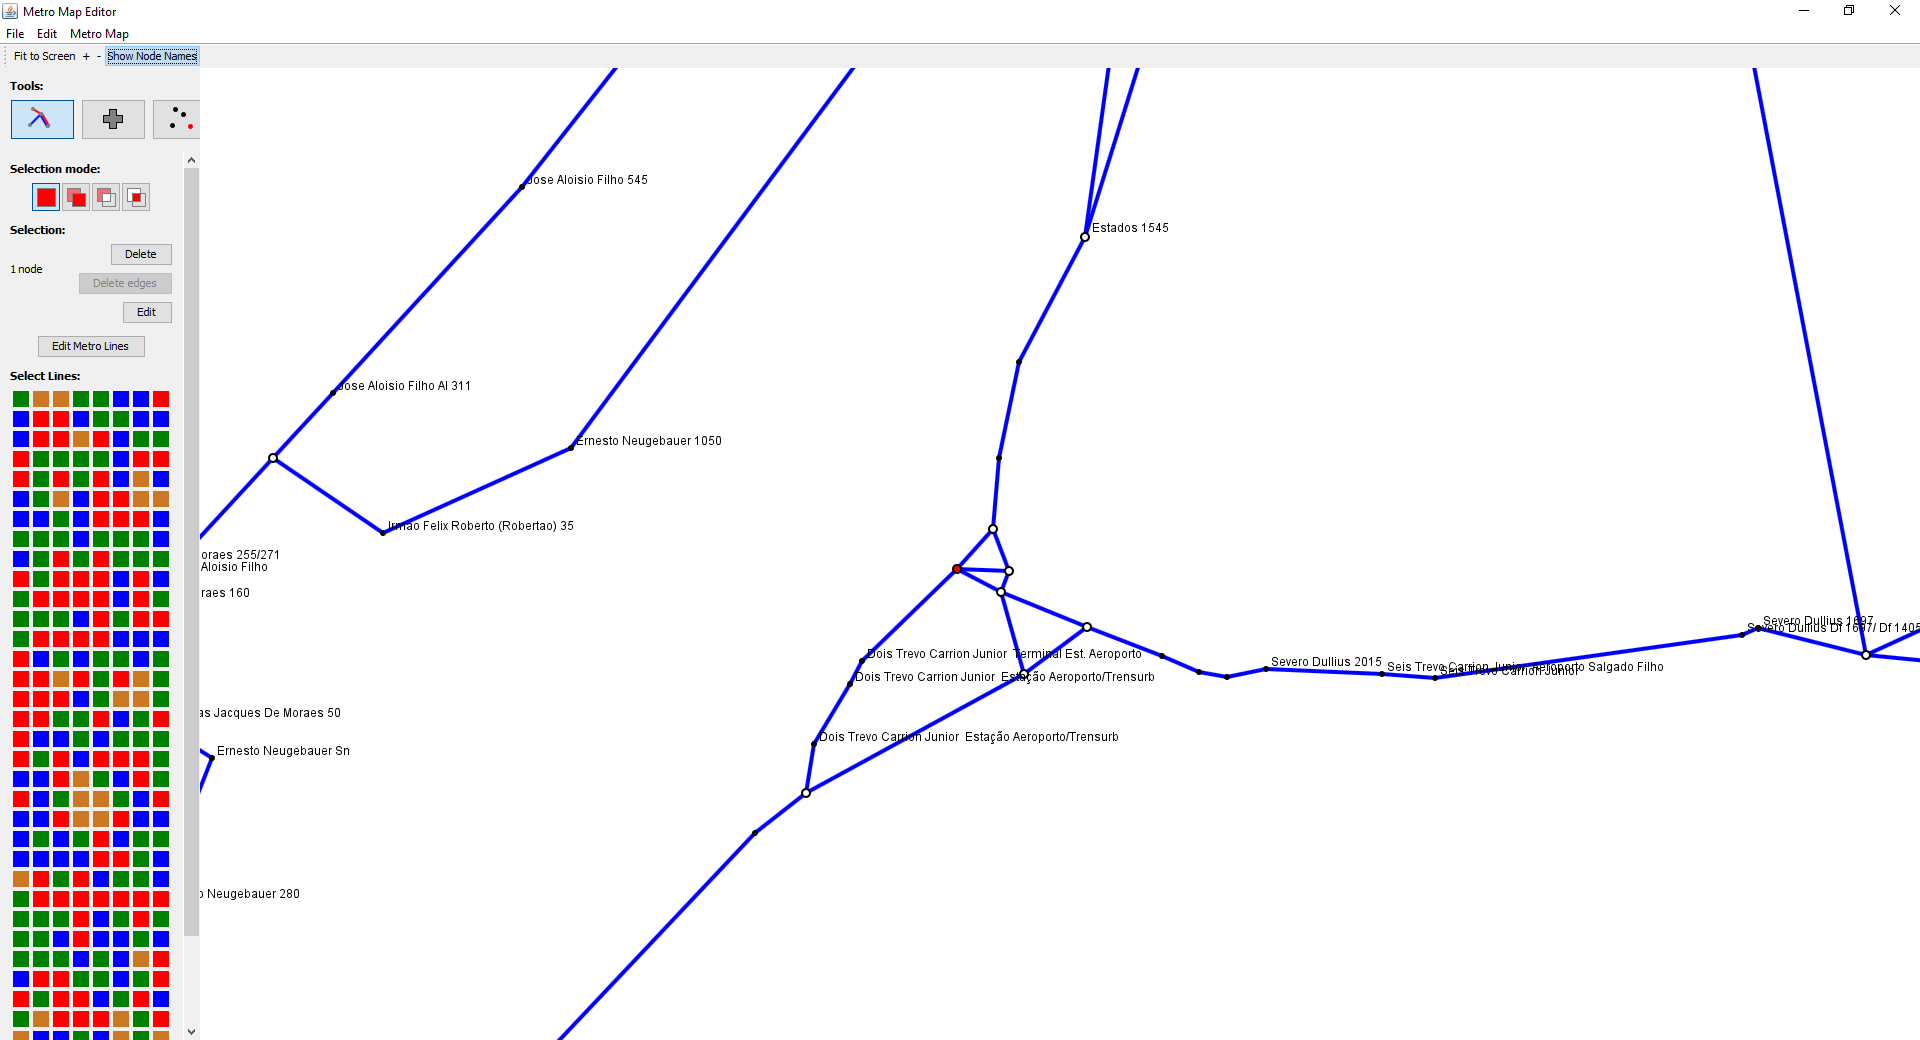
\includegraphics[width=\linewidth, trim=562 100 560 160, clip]{imagens/abstracao_depois.png}
        \subcaption{Depois da fusão.}
    \end{minipage}
    \vspace{0.5cm}
    \caption{Ilustração prática da fusão de paradas próximas na rede de transporte, utilizando a região norte do aeroporto Salgado Filho como exemplo.}
    \label{fig:fusao_pratica}
\end{figure}

\subsection{Remoção de Paradas Adjacentes}
\label{subsec:remocao_paradas_adjacentes}

Uma técnica de abstração, mencionada por autores como Nöllenburg e Wolff, consiste na remoção de paradas sequenciais para reduzir a complexidade do problema. Os vértices removidos podem, então, ser re-inseridos de forma posterior ao solver MIP em uma etapa de pós-processamento.

No entanto, a aplicação irrestrita dessa estratégia em uma rede de alta densidade, como a de ônibus de Porto Alegre, revela-se ser problemática. Diferentemente das redes de metrô, cujos traçados são predominantemente retilíneos, as rotas de ônibus seguem a geometria curvilínea das vias urbanas. A remoção total de paradas adjacentes comprometeria a representação visual dessas curvas, prejudicando a legibilidade do mapa e a preservação do mapa mental do usuário.

Para a remoção de vértices adjacentes, adotou-se um critério angular. Vértices que formam ângulos (denominados por $\varphi$) excessivamente agudos são eliminados, pois representam curvas desnecessárias que podem prejudicar a construção do mapa mental do usuário. Similarmente, vértices com $\varphi$ excessivamente obtuso são removidos, uma vez que já se assemelham a segmentos de reta. Essa lógica é implementada por meio de limites angulares inferior ($\varphi_{\min} = 80^\circ$) e superior ($\varphi_{\max} = 150^\circ$), conforme esquematizado na Figura~\ref{fig:criterio_angular}. No cenário ilustrado, considerando-se os vértices $A$ e $B$ conectados e três posicionamentos possíveis para um vértice adjacente subsequente $C$, avalia-se o ângulo de inflexão $\varphi = \angle CAB$: caso $C$ recaia na região em vermelho, formando um ângulo superior a $\varphi_{\max} = 150^\circ$ (quase colinear) ou inferior a $\varphi_{\min} = 80^\circ$ (curva excessivamente fechada), o nó intermediário $A$ é removido, estabelecendo-se uma ligação direta entre $C$ e $B$; por outro lado, caso $\varphi$ situe-se no setor em verde ($\varphi_{\min} \le \varphi \le \varphi_{\max}$, isto é, entre $80^\circ$ e $150^\circ$), o vértice $A$ é mantido no grafo para preservar a geometria da via.

\begin{figure}[H]
    \centering
    \vspace{0.5cm}
    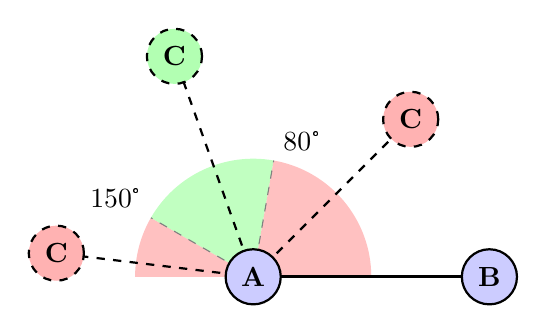
\begin{tikzpicture}[node_style/.style={circle, draw, thick, fill=blue!20, minimum size=0.7cm, inner sep=0pt, font=\bfseries}]
        % Coordenadas dos nós base
        \coordinate (A) at (0,0);
        \coordinate (B) at (3,0);
        \coordinate (C) at (-2.5,0.3);
        \coordinate (D) at (-1.0,2.8);
        \coordinate (E) at (2,2);

        % Raio para os setores angulares
        \def\auraradius{1.5cm}

        % Desenha os setores de decisão preenchidos (fica no fundo)
        \fill[red!30, opacity=0.8] (A) -- ($(A)+(150:\auraradius)$) arc (150:180:\auraradius) -- cycle;
        \fill[green!30, opacity=0.8] (A) -- ($(A)+(80:\auraradius)$) arc (80:150:\auraradius) -- cycle;
        \fill[red!30, opacity=0.8] (A) -- ($(A)+(0:\auraradius)$) arc (0:80:\auraradius) -- cycle;

        % Linhas e rótulos dos ângulos limítrofes (fundo, atrás das arestas)
        \draw[gray, dashed] (A) -- ($(A)+(80:\auraradius)$);
        \node[above right] at ($(A)+(80:\auraradius)$) {80°};
        \draw[gray, dashed] (A) -- ($(A)+(150:\auraradius)$);
        \node[above left] at ($(A)+(150:\auraradius)$) {150°};

        % PRIMEIRO as arestas...
        \draw[very thick] (A) -- (B);
        \draw[thick, dashed] (A) -- (C);
        \draw[thick, dashed] (A) -- (D);
        \draw[thick, dashed] (A) -- (E);

        % ...DEPOIS os nós, para ficarem por cima
        \node[node_style] at (A) {A};
        \node[node_style] (b_node) at (B) {B};
        \node[node_style, fill=red!30, dashed] at (C) {C};
        \node[node_style, fill=green!30, dashed] at (D) {C};
        \node[node_style, fill=red!30, dashed] at (E) {C};

    \end{tikzpicture}
    \caption{Ilustração do critério angular para remoção de vértices com base no ângulo $\varphi$. Setores coloridos indicam a decisão: quando $\varphi$ recai na faixa verde ($\varphi_{\min} \le \varphi \le \varphi_{\max}$, com $80^\circ \le \varphi \le 150^\circ$), o nó é mantido para preservar a geometria; caso $\varphi$ situe-se nas faixas vermelhas ($\varphi < 80^\circ$ ou $\varphi > 150^\circ$), o vértice intermediário é removido.}
    \label{fig:criterio_angular}
\end{figure}

O impacto visual dessas abordagens é contrastado na Figura~\ref{fig:comparativo_remocao} sobre o subsistema das Linhas Transversais: a Figura~\ref{fig:adj_antes} exibe a malha inicial sem nenhuma remoção de paradas adjacentes; a Figura~\ref{fig:adj_total} retrata o resultado da remoção de todos os vértices adjacentes de grau 2; e a Figura~\ref{fig:adj_limiar} apresenta a simplificação guiada pela heurística angular $\varphi$ proposta nesta seção. Observa-se que, enquanto a eliminação irrestrita e total de nós intermediários provoca uma simplificação excessiva que achata o traçado e descaracteriza a geometria original das vias, o critério angular $\varphi \in [80^\circ, 150^\circ]$ estabelece um equilíbrio eficiente, reduzindo substancialmente a densidade do grafo sem comprometer as curvas essenciais para a orientação espacial do usuário.


\begin{figure}[H]
    \centering
    \begin{subfigure}[b]{0.32\textwidth}
        \centering
        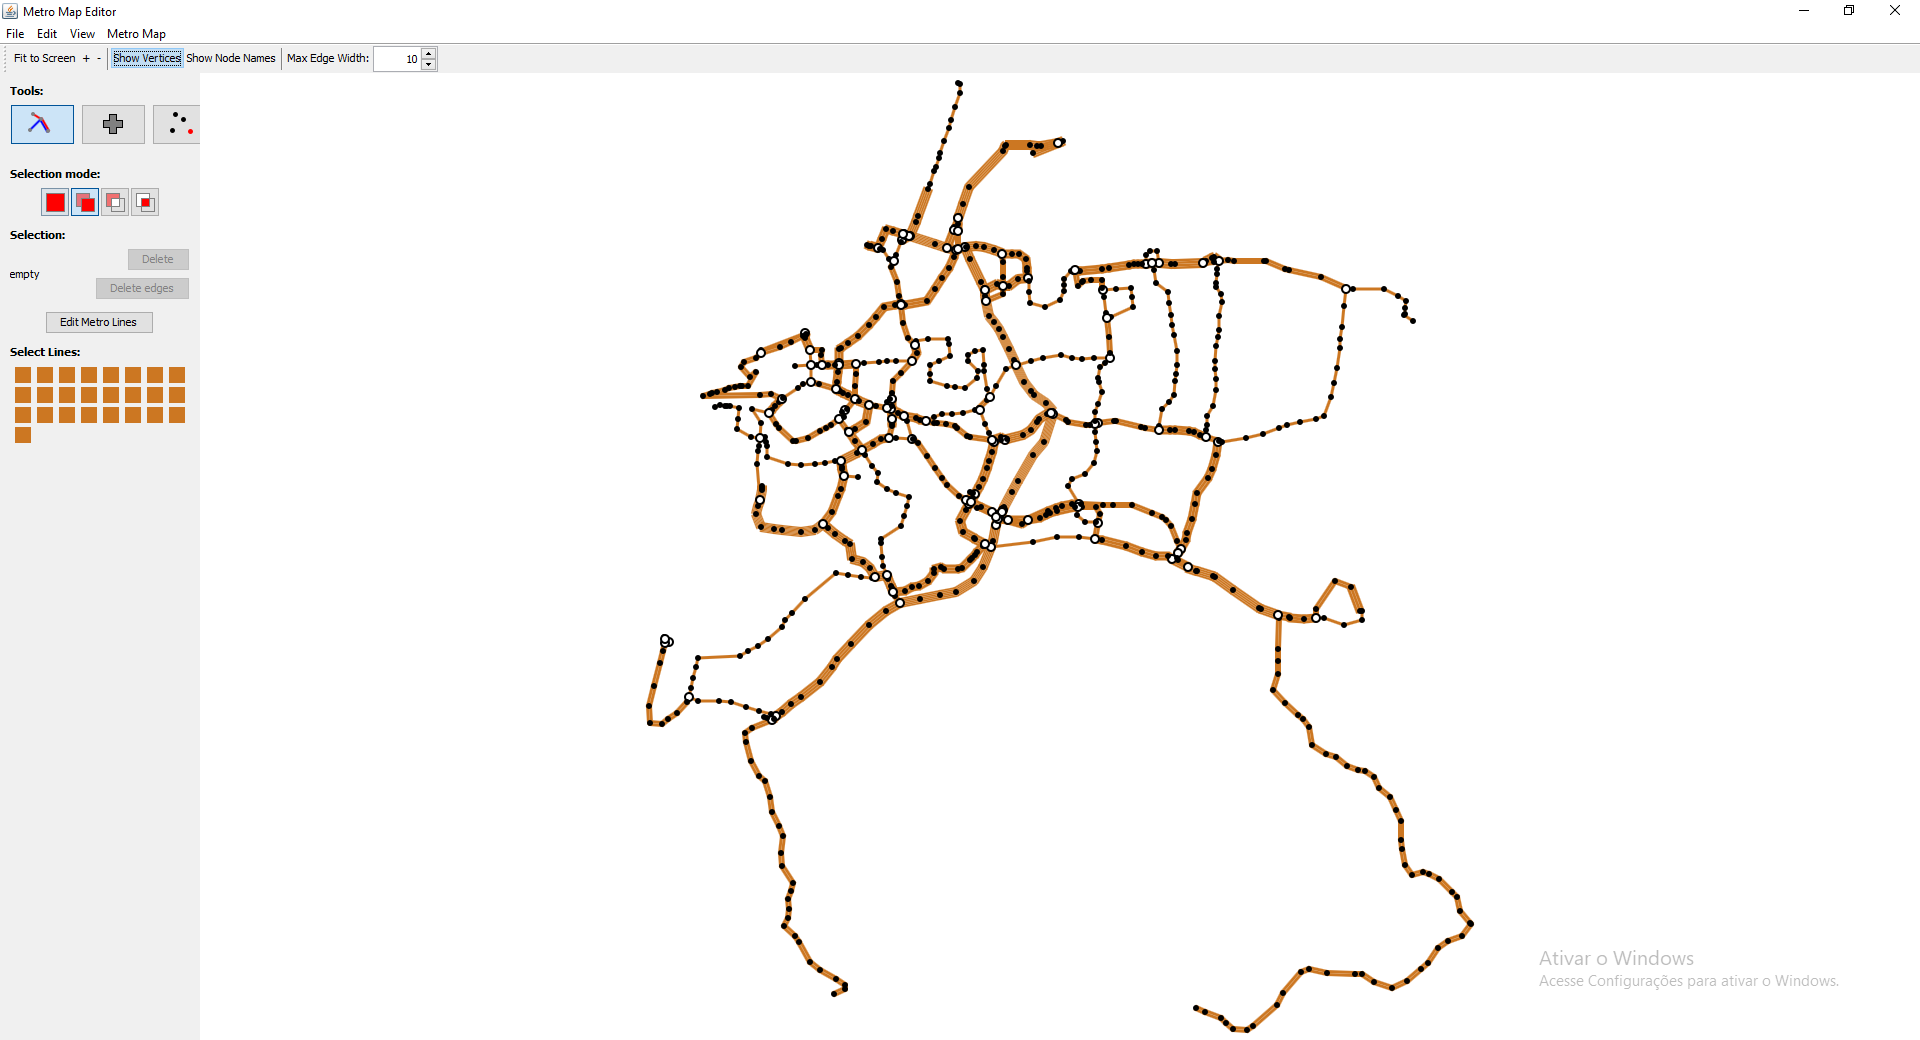
\includegraphics[width=\linewidth, trim=450 0 330 60, clip]{imagens/adjacentes_antes.png}
        \caption{Mapa original.}
        \label{fig:adj_antes}
    \end{subfigure}
    \hfill
    \begin{subfigure}[b]{0.32\textwidth}
        \centering
        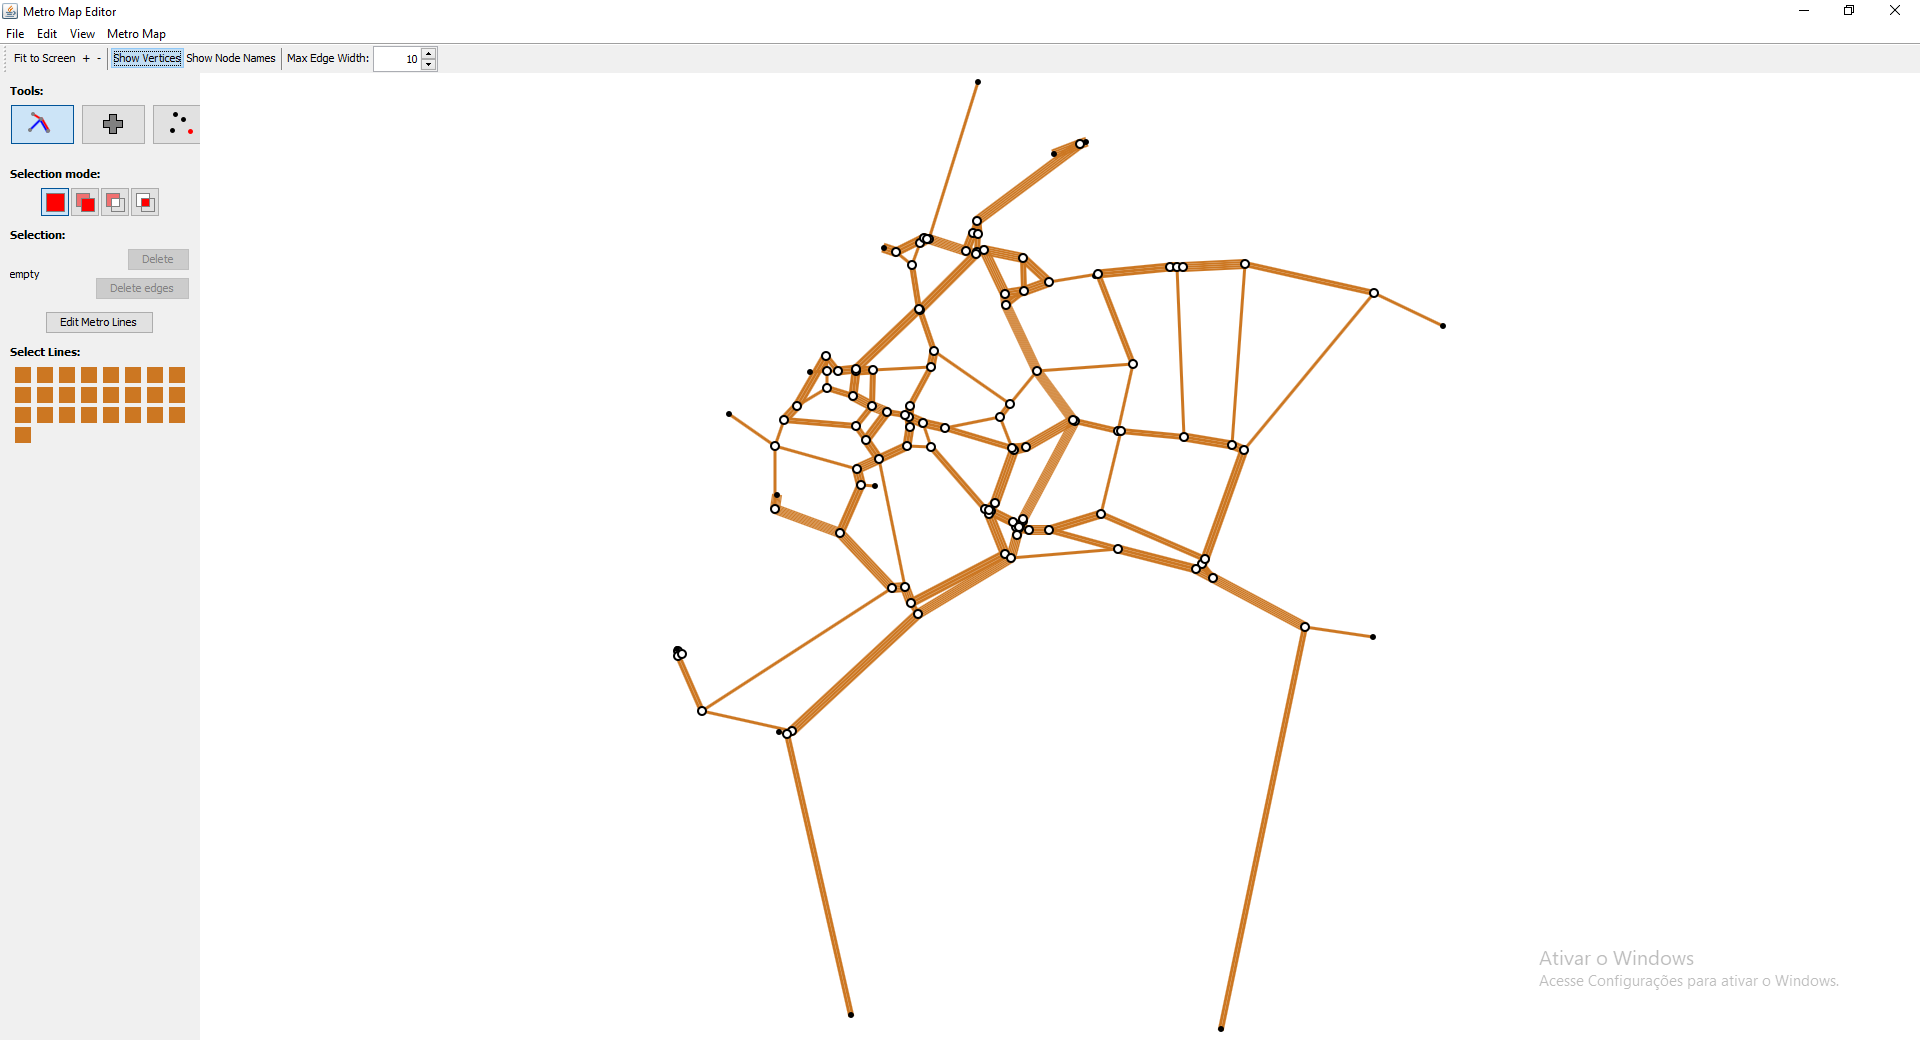
\includegraphics[width=\linewidth, trim=450 0 330 60, clip]{imagens/adjacentes_tudo.png}
        \caption{Remoção total.}
        \label{fig:adj_total}
    \end{subfigure}
    \hfill
    \begin{subfigure}[b]{0.32\textwidth}
        \centering
        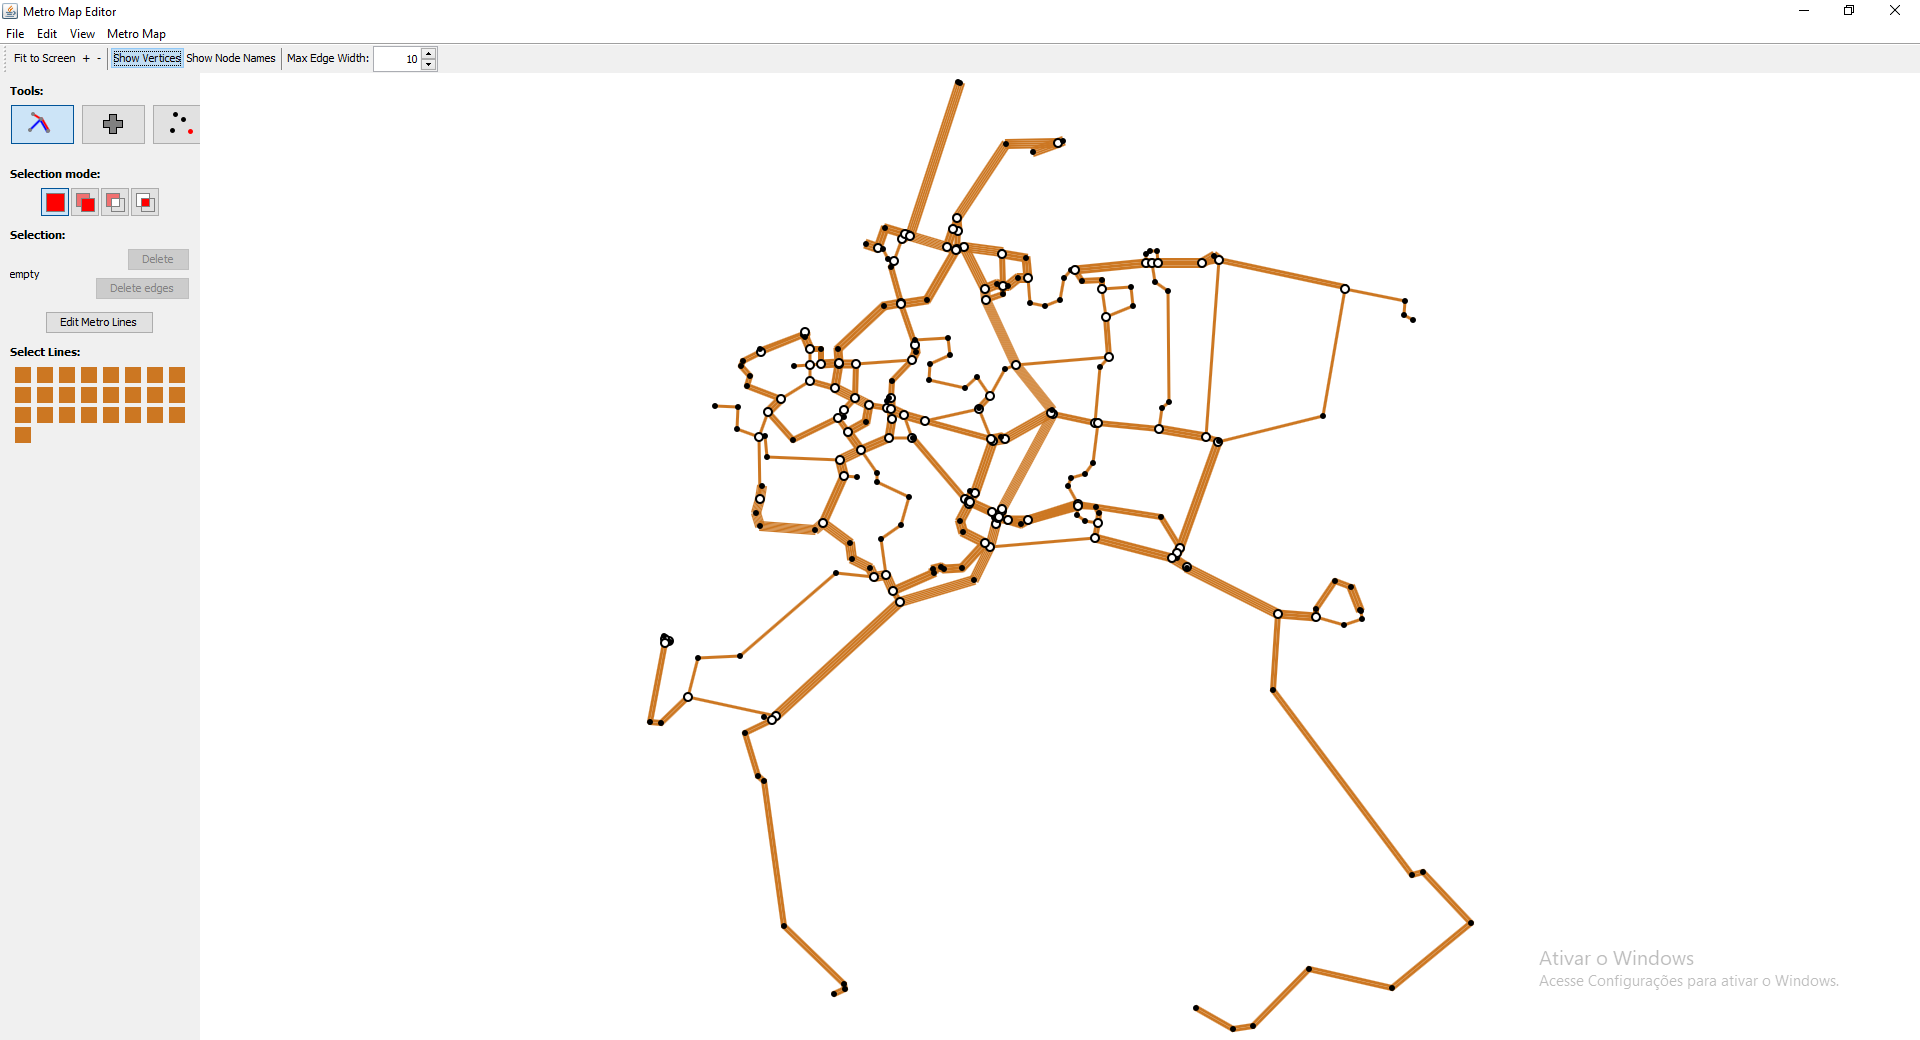
\includegraphics[width=\linewidth, trim=450 0 330 60, clip]{imagens/adjacentes_limiar.png}
        \caption{Remoção por limiar ($\varphi$).}
        \label{fig:adj_limiar}
    \end{subfigure}
    \caption{Comparativo das estratégias de remoção de vértices adjacentes: (a) mapa original; (b) remoção irrestrita total, que compromete a geometria; e (c) simplificação orientada pelo limiar angular $\varphi$, que preserva as curvas essenciais.}
    \label{fig:comparativo_remocao}
\end{figure}


\section{Modelo de Otimização Adaptado}
\label{sec:modelo_otimizacao}

A formulação matemática desenvolvida neste trabalho fundamenta-se no modelo de Programação Linear Inteira Mista (MIP) proposto por Nöllenburg e Wolff \cite{Nollenburg}. Embora a formulação original tenha sido concebida primariamente para sistemas ferroviários e metropolitanos compostos por grafos de escala moderada, sua aplicação à malha de ônibus de Porto Alegre demandou adaptações estruturais tanto no conjunto de restrições geométricas quanto na condução do processo de otimização.

O principal gargalo computacional do modelo original reside no conjunto de restrições rígidas que impedem o cruzamento entre arestas não adjacentes (Equações~\ref{eq:crossing_sum} e~\ref{eq:crossing_coord}). A imposição de não-cruzamento exibe complexidade quadrática em relação ao número de arestas ($O(|E|^2)$), tornando-se o componente mais custoso da formulação e inviabilizando a convergência do solver em instâncias de grande porte. Diversos trabalhos que extendem o de Nöllenburg desativam estas restrições, já que em malhas ferroviárias a supressão dessas restrições raramente acarreta sobreposições indesejadas. Contudo em grafos densos de ônibus a desativação total resulta em fortes distorções na geometria final, degradando o posicionamento relativo entre vértices não adjacentes. Para contornar essa limitação sem reintroduzir o custo quadrático no solver, foi desenvolvida uma etapa iterativa voltada a identificar e corrigir vértices excessivamente distorcidos, baseada na ideia de Nöllenburg restaurando a coerência espacial do mapa esquemático.

Para avaliar diferentes compromissos de desempenho e qualidade visual, o presente trabalho estruturou duas variantes do pipeline de otimização MIP: a \textbf{versão biobjetiva} e a \textbf{versão triobjetiva}. A herança metodológica de cada versão define-se de forma direta: a \textbf{versão biobjetiva} herda integralmente a formulação de Oke e Siddiqui~\cite{Oke}, otimizando apenas curvas e posição relativa sob restrição rígida de comprimento das arestas; já a \textbf{versão triobjetiva} utiliza as mesmas melhorias e simplificações de Oke e Siddiqui~\cite{Oke}, mas resgata de Nöllenburg e Wolff~\cite{Nollenburg} a modelagem do comprimento das arestas como uma \textit{soft constraint} na função objetivo, sem transformá-la em uma \textit{hard constraint}. Em ambas as formulações, as restrições rígidas de cruzamento de complexidade quadrática ($O(|E|^2)$) de Nöllenburg e Wolff são suprimidas e substituídas pela correção iterativa angular proposta neste trabalho.

\subsection{Correção Iterativa de Distorções Geométricas}
\label{subsec:correcao_distorcoes}

Para mitigar o custo computacional das restrições de não-cruzamento em redes ferroviárias, Nöllenburg e Wolff \cite{Nollenburg} propõem uma estratégia iterativa: o modelo é inicialmente resolvido sem tais restrições e, caso cruzamentos indevidos sejam detectados no layout resultante, restrições de separação espacial são adicionadas sob demanda apenas para os pares de arestas conflitantes, reotimizando o mapa até a eliminação das sobreposições.

No caso da rede de ônibus de Porto Alegre, contudo, a eliminação sistemática de cruzamentos entre arestas não adjacentes mostrou-se computacionalmente proibitiva diante da elevada densidade da malha, inviabilizando a convergência do solver mesmo através de abordagens sob demanda. Como alternativa substancialmente mais barata para assegurar a preservação da topologia global e conter deformações espaciais severas, adaptou-se o paradigma iterativo para atuar mediante a verificação de nós não adjacentes sob duas condições. Primeiramente, identifica-se se os vértices ficaram espacialmente sobrepostos no layout, isto é, com distância sob a norma $L_\infty$ inferior ao comprimento mínimo de aresta $\ell_{uv}$. Em segundo lugar, avalia-se a variação angular do vetor formado entre os dois nós antes e após a otimização, mensurada pelo desvio angular $|\Delta\theta|$. Conforme ilustrado na Figura~\ref{fig:criterio_angular_pos_processamento}, adota-se um limiar de tolerância angular $|\Delta\theta| \le 100^\circ$. Caso os nós estejam sobrepostos ou sua divergência angular $|\Delta\theta|$ ultrapasse o limiar tolerado (isto é, $|\Delta\theta| > 100^\circ$, situando-se na região de distorção severa), introduz-se uma restrição corretiva como a apresentada na Equação~\ref{eq:pos_restricao_direcao}, forçando o par de vértices a respeitar uma distância mínima $\ell_{uv}$ ao longo da orientação original e reotimizando o layout de maneira direcionada.

\begin{align}
x(v) &\ge - x(u) + \ell_{uv}. \label{eq:pos_restricao_direcao} \\
&\vdots \nonumber
\end{align}

\begin{figure}[H]
    \centering
    \vspace{0.3cm}
    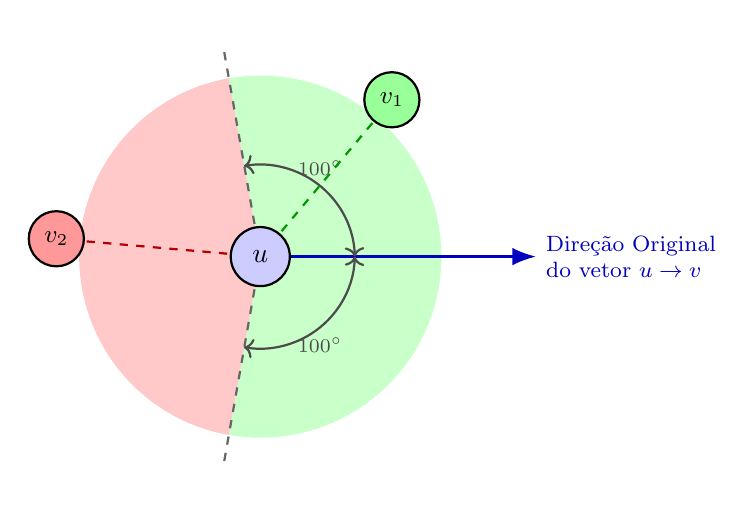
\begin{tikzpicture}[
        node_style/.style={circle, draw, thick, fill=blue!20, minimum size=0.75cm, inner sep=0pt, font=\bfseries},
        sample_node/.style={circle, draw, thick, minimum size=0.7cm, inner sep=0pt, font=\bfseries\small}
    ]
        % Coordenadas base
        \coordinate (U) at (0,0);
        \def\auraradius{2.3cm}

        % Setores angulares de decisão
        % Setor aceitável: de -135° até +135° (arco de 270°)
        \fill[green!25, opacity=0.85] (U) -- ($(U)+(-100:\auraradius)$) arc (-100:100:\auraradius) -- cycle;
        % Setor de violação / distorção excessiva: de 135° até 225° (-135°)
        \fill[red!25, opacity=0.85] (U) -- ($(U)+(100:\auraradius)$) arc (100:260:\auraradius) -- cycle;

        % Linhas tracejadas dos limites angulares de 135°
        \draw[gray!80!black, dashed, thick] (U) -- ($(U)+(100:\auraradius+0.4cm)$) node[above left, font=\footnotesize] {};
        \draw[gray!80!black, dashed, thick] (U) -- ($(U)+(-100:\auraradius+0.4cm)$) node[below left, font=\footnotesize] {};

        % Vetor da direção original (eixo de referência a 0°)
        \draw[-{Latex[length=3mm]}, thick, blue!75!black] (U) -- (3.5,0) node[right, font=\footnotesize, align=left] {Direção Original\\do vetor $u \to v$};

        % Arcos indicando o limiar de tolerância angular
        \draw[<->, thick, gray!60!black] ($(U)+(0:1.2cm)$) arc (1.5:100:1.2cm) node[midway, above, font=\scriptsize] {$100^\circ$};
        \draw[<->, thick, gray!60!black] ($(U)+(0:1.2cm)$) arc (-1.5:-100:1.2cm) node[midway, below, font=\scriptsize] {$100^\circ$};

        % Exemplo de vértice pós-otimização ACEITO (dentro do limiar <= 135°)
        \coordinate (V_ok) at (50:2.6cm);
        \draw[thick, dashed, green!60!black] (U) -- (V_ok);
        \node[sample_node, fill=green!40] at (V_ok) {$v_1$};
        \node[above right, font=\footnotesize, text=green!50!black] at (V_ok) {};

        % Exemplo de vértice pós-otimização DISTORCIDO (fora do limiar > 135°)
        \coordinate (V_bad) at (175:2.6cm);
        \draw[thick, dashed, red!70!black] (U) -- (V_bad);
        \node[sample_node, fill=red!40] at (V_bad) {$v_2$};
        \node[left, font=\footnotesize, text=red!60!black, align=right] at ($(V_bad)+(-0.1,0.25)$) {};

        % Nó base u
        \node[node_style] at (U) {$u$};

    \end{tikzpicture}
    \caption{Critério angular para identificação de distorções em vértices não adjacentes com base no desvio $|\Delta\theta|$. A região verde delimita a faixa de tolerância angular ($|\Delta\theta| \le 100^\circ$) em relação à orientação original. Um vértice $v$, se posicionado em $v_1$ após a otimização, permanece aceito; contudo, caso assuma uma posição como $v_2$, adentra a região crítica por configurar distorção geométrica severa ($|\Delta\theta| > 100^\circ$), tornando-se sujeito à inclusão da restrição corretiva no MIP.}
    \label{fig:criterio_angular_pos_processamento}
\end{figure}

A aplicação iterativa dessa restrição corretiva mostra-se eficaz na mitigação das distorções espaciais, conferindo ao grafo uma forma global substancialmente mais fiel à geografia original da rede. Ademais, por se tratar de uma restrição linear direta, sua adição acarreta um impacto mínimo no esforço computacional exigido do solver, viabilizando a execução fluida de múltiplos ciclos de refinamento incremental. Limiares de tolerância angular $|\Delta\theta|$ inferiores a $100^\circ$ foram avaliados experimentalmente; no entanto, configurações mais restritivas provocaram a inserção de uma quantidade excessiva de restrições no modelo, degradando o tempo de convergência, o que motivou a fixação de $100^\circ$ como o ponto de equilíbrio ideal. A comprovação da eficácia dessa estratégia na estabilização topológica da malha viária é analisada na Seção~\ref{subsec:analise_correcao_iterativa}.

\subsection{Tratamento de Paradas Intermediárias}

A remoção temporária de paradas na etapa de simplificação topológica (Seção~\ref{subsec:remocao_paradas_adjacentes}) faz com que uma única aresta $(u, v)$ no grafo simplificado passe a representar um trajeto que continha múltiplos nós na malha original. Para assegurar que haja espaçamento adequado para a futura reinserção dessas estações sem comprometer a legibilidade, o comprimento mínimo dessa aresta (originalmente estabelecido na Equação~\ref{eq:octi_coords}) deve ser proporcional à quantidade de paradas suprimidas.

Dessa forma, o limite inferior de distância é ajustado para $\ell_{uv} \cdot (k + 1)$, onde $k$ representa o número de vértices intermediários removidos daquele segmento. A formulação matemática dessa restrição é expressa no conjunto de inequações em~\ref{eq:octi_coords_intermediarios}, onde $M$ é uma constante de valor elevado (Big-$M$) e $\alpha_{\text{i}}$ é a variável binária associada à direção selecionada:

\begin{align}
y(u) - y(v) &\le M(1 - \alpha_{\text{i}}(u, v)), && \forall (u, v) \in E, \; \forall i \in \{\text{prec}, \text{orig}, \text{succ}\} \label{eq:octi_coords_intermediarios} \\
-y(u) + y(v) &\le M(1 - \alpha_{\text{i}}(u, v)), \nonumber \\
x(u) - x(v) &\ge -M(1 - \alpha_{\text{i}}(u, v)) + \ell_{uv} \cdot (k + 1). \nonumber \\
&\vdots \nonumber
\end{align}

Concluída a resolução pelo solver MIP, os $k$ vértices intermediários são reincorporados ao grafo por meio de uma interpolação linear equidistante ao longo do segmento resultante $(u, v)$, preservando rigorosamente a ordem topológica e a integridade do trajeto original. 

\subsection{Modelo de Oke}
\label{sec:modelo_oke}

Dentre as abordagens encontradas na literatura, a formulação proposta por Oke e Siddiqui \cite{Oke} destacou-se como a mais promissora para aplicação à malha viária de Porto Alegre, em razão de seu foco principal em eficiência computacional. Essa abordagem introduz simplificações estruturais em relação ao modelo de Nöllenburg e Wolff \cite{Nollenburg}, sendo o principal diferencial a reestruturação de sua função objetivo, que passa a otimizar apenas duas restrições flexíveis (\textit{soft constraints}) em detrimento das três contempladas originalmente, as modificações são conforme detalhado a seguir.

A primeira alteração fundamental ocorre na função objetivo de Nöllenburg e Wolff (Equação~\ref{eq:funcao_objetivo_nollenburg}), da qual se elimina a penalidade de extensão das arestas ($C_{\text{len}}$). Essa modificação converte o modelo em uma formulação estritamente biobjetiva, concentrando o esforço de otimização na minimização de curvas e na preservação da orientação angular relativa, conforme expresso na Equação~\ref{eq:funcao_objetivo_oke}:

\begin{equation}
\min \quad w_{\text{bends}} \cdot C_{\text{bends}} + w_{\text{rpos}} \cdot C_{\text{rpos}}.
\label{eq:funcao_objetivo_oke}
\end{equation}

Em substituição à penalidade flexível, o controle sobre o comprimento dos segmentos passa a ser imposto como uma restrição rígida (\textit{hard constraint}) que estabelece um limite superior ($\ell_{\max}$) para as arestas. Para assegurar espaço suficiente à reinserção posterior dos nós suprimidos, esse teto é igualmente parametrizado em função da quantidade $k$ de vértices intermediários pertencentes ao trecho, estipulando $\ell_{\max}(u, v) = L_{\max} \cdot \ell_{uv} \cdot (k + 1)$. A implementação dessa restrição é descrita pelo conjunto de inequações em~\ref{eq:oke_limite_maximo}:

\begin{align}
x(u) - x(v) &\le L_{\max} \cdot \ell_{uv} \cdot (k + 1), && \forall (u, v) \in E \label{eq:oke_limite_maximo} \\
-x(u) + x(v) &\le L_{\max} \cdot \ell_{uv} \cdot (k + 1), \nonumber \\
y(u) - y(v) &\le L_{\max} \cdot \ell_{uv} \cdot (k + 1), \nonumber \\
-y(u) + y(v) &\le L_{\max} \cdot \ell_{uv} \cdot (k + 1). \nonumber
\end{align}

A definição do multiplicador $L_{\max} = 4$ resultou de calibrações empíricas. O objetivo foi adotar o menor limitador possível que ainda conferisse ao modelo a factibilidade por meio do solver, visto que algumas distorções nos comprimentos das vias são, por vezes, necessárias para manter características visuais mais desejadas como a retilineidade.

Outra contribuição fundamental do modelo de Oke e Siddiqui reside na relaxação da integralidade das coordenadas ($x, y$), declarando-as como variáveis contínuas reais ($x, y \in \mathbb{R}$) em vez de variáveis inteiras. Os autores demonstram que, devido à imposição estrita da octilinearidade (ângulos múltiplos de $45^\circ$) combinada com parâmetros de comprimento e separação inteiros ($\ell_{uv}$ e $\ell_{\max}$), as soluções ótimas encontradas pelo solver convergem naturalmente para a grade geométrica, sem a necessidade de forçar a integralidade dessas variáveis. Essa formulação converte o Programa Inteiro Misto (\textit{MIP}) em um Programa Linear Misto Binário, no qual apenas as variáveis direcionais e topológicas de decisão ($\alpha, \beta, \gamma, \delta$) permanecem discretas. Sob a ótica de desempenho, essa simplificação livra a árvore de busca do CPLEX de ramificar sobre variáveis de posição, reduzindo expressivamente o número de nós explorados e acelerando o tempo de resolução.

Por fim, em relação à resolução multiobjetivo, Oke e Siddiqui propõem a utilização do método $\epsilon$-restrito aumentado (\textit{AUGMECON2})~\cite{MAVROTAS20139652} como alternativa à tradicional combinação linear por pesos. Enquanto a abordagem por pesos adotada por Nöllenburg e Wolff depende da calibração empírica de coeficientes e gera apenas um único layout por execução, o método AUGMECON2 otimiza diretamente um objetivo principal (como a minimização de curvas $C_{\text{bends}}$) enquanto trata o objetivo secundário (a preservação da orientação geográfica $C_{\text{rpos}}$) como uma restrição cujo limite varia sistematicamente. Essa estratégia permite explorar e gerar de forma automatizada um conjunto de soluções alternativas em uma única execução, disponibilizando opções de mapas com diferentes graus de equilíbrio entre simplicidade visual (linhas mais retas) e fidelidade geográfica, sem a necessidade de arbitrar pesos manualmente.

Contudo, a aplicação do método AUGMECON2 mostrou-se incompatível com o algoritmo de correção iterativa de distorções geométricas proposto neste trabalho (Seção~\ref{subsec:correcao_distorcoes}). Como o AUGMECON2 opera através da resolução sequencial de dezenas de subproblemas MIP, sua incorporação exigiria executar essa varredura completa a cada ciclo de adição de restrições angulares, elevando o tempo total de processamento a níveis proibitivos. Diante desse custo computacional acumulado, optou-se por não utilizar o AUGMECON2 no pipeline final, preservando a abordagem de combinação linear ponderada por pesos (Equação~\ref{eq:funcao_objetivo_oke}), a qual viabiliza a execução rápida de uma única instância por ciclo iterativo.

\section{Exportação e Formato de Saída}
\label{sec:exportacao}

Após a resolução do modelo pelo solver CPLEX, as novas coordenadas dos vértices resultantes do processo de otimização precisam ser convertidas em uma representação gráfica apropriada. Conforme apresentado no fluxo geral da arquitetura (Figura~\ref{fig:fluxo_arquitetura}), a exportação dos resultados é realizada pelo módulo \texttt{gtfs\_to\_xml.jl}, que transforma o grafo gerado no formato GraphML, um padrão aberto baseado em XML amplamente utilizado para a descrição e intercâmbio de estruturas de grafos.

A escolha do padrão GraphML assegura a compatibilidade direta com a ferramenta de visualização gráfica (GUI) em Java desenvolvida por Nöllenburg, a qual utiliza a biblioteca JUNG (\textit{Java Universal Network/Graph Framework}) para o processamento e a renderização interativa dos diagramas esquemáticos. Para que a interface interprete corretamente a geometria, a topologia e a identidade visual de cada linha de ônibus, a saída é codificada seguindo a estrutura descrita a seguir:

\begin{itemize}
    \item \textbf{Definição de Atributos (\texttt{<key>}):} No cabeçalho do documento XML, são declaradas as propriedades associadas aos elementos do grafo:
    \begin{itemize}
        \item \textbf{Atributos de Vértices:} São definidos os atributos \texttt{x} e \texttt{y} (coordenadas no plano, do tipo \texttt{double}) e \texttt{label} (identificador textual da estação ou parada, do tipo \texttt{string}).
        \item \textbf{Atributos de Arestas:} Para cada linha de ônibus presente na rede, cria-se uma chave booleana identificadora (e.g., \texttt{l\_T1}). A declaração dessa chave também armazena metadados visuais, como o nome curto e a cor da linha em notação hexadecimal, utilizados pela GUI para desenhar as faixas paralelas coloridas ao longo das arestas.
    \end{itemize}
    \item \textbf{Declaração dos Elementos do Grafo:}
    \begin{itemize}
        \item \textbf{Nós (\texttt{<node>}):} Cada vértice do grafo gerado pelo modelo é representado por um elemento contendo seu identificador exclusivo, suas coordenadas calculadas ($x, y$) e seu respectivo rótulo (\textit{label}).
        \item \textbf{Arestas (\texttt{<edge>}):} Cada segmento da malha conecta um nó de origem (\texttt{source}) a um nó de destino (\texttt{target}). Dentro do elemento da aresta, elementos \texttt{<data>} ativam (com valor \texttt{true}) as chaves booleanas correspondentes a cada uma das linhas de transporte que trafegam naquele trecho.
    \end{itemize}
\end{itemize}

Essa padronização viabiliza a renderização fiel das rotas sobrepostas e permite inspecionar visualmente a eficácia da simplificação geométrica e topológica obtida pelo modelo MIP.

\chapter{Resultados e Análise}
\label{cap:resultados}

Neste capítulo, são apresentados e discutidos os resultados obtidos a partir da aplicação do modelo matemático e do pipeline de esquematização propostos sobre a malha de transporte coletivo por ônibus de Porto Alegre. O objetivo central é avaliar a viabilidade prática da metodologia desenvolvida, confrontando a qualidade estética e topológica dos diagramas gerados com o respectivo custo computacional de resolução.

\section{Configuração dos Experimentos}
\label{sec:configuracao_experimentos}

Para avaliar a viabilidade computacional, a escalabilidade e a qualidade estética da metodologia proposta, foram conduzidos experimentos quantitativos e qualitativos sobre a malha de transporte público por ônibus de Porto Alegre. Esta seção detalha o ambiente computacional, as características dos dados submetidos, os parâmetros de calibração do modelo MIP e do solver, bem como as métricas adotadas para a análise dos resultados.
\subsection{Ambiente Computacional}
\label{subsec:ambiente_computacional}

A implementação do pipeline de pré-processamento, a instanciação do modelo matemático e o algoritmo iterativo de correção angular foram desenvolvidos na linguagem Julia~\cite{bezanson2017julia}. O modelo de otimização foi formulado através do pacote de modelagem matemática \texttt{JuMP.jl}~\cite{lubin2023jump}, integrado ao solver comercial IBM ILOG CPLEX (versão~22.1.1.0)~\cite{cplex2022} por meio da biblioteca \texttt{CPLEX.jl}. A inspeção visual dos mapas e a validação qualitativa das rotas foram realizadas na interface gráfica em Java desenvolvida por Nöllenburg, mediante a leitura de arquivos estruturados no formato GraphML~\cite{brandes2010graph}.

Todos os experimentos de otimização foram executados em um nó de processamento do cluster Phoenix, alocado no Laboratório de Computação de Alto Desempenho (PCAD) da UFRGS, cujas especificações de hardware estão detalhadas na Tabela~\ref{tab:hardware_phoenix}. Nos experimentos conduzidos, foram alocadas 44 das 48 threads disponíveis para execução paralela do solver.

\begin{table}[H]
    \centering
    \caption{Especificações de hardware do nó computacional utilizado no PCAD.}
    \label{tab:hardware_phoenix}
    \resizebox{\linewidth}{!}{%
    \begin{tabular}{llllll}
        \toprule
        \textbf{Partição} & \textbf{CPU} & \textbf{RAM} & \textbf{Acelerador} & \textbf{Disco} & \textbf{Placa-mãe} \\
        \midrule
        \texttt{phoenix} & 2 $\times$ Intel Xeon Gold 5317, 3,0\,GHz (24 \textit{cores}, 48 \textit{threads}) & 128\,GB DDR4 & --- & 223,6\,GB SSD & Supermicro X12DPL-NT6 \\
        \bottomrule
    \end{tabular}%
    }
\end{table}
\subsection{Dados e Instâncias de Teste}
\label{subsec:dados_instancias}

A base de dados experimental é constituída pelos dados oficiais no formato GTFS disponibilizados pela Empresa Pública de Transporte e Circulação (EPTC) de Porto Alegre~\cite{EPTCGTFS}. No padrão adotado pela EPTC, as rotas são categorizadas e codificadas visualmente conforme a divisão operacional do sistema municipal:
\begin{itemize}
    \item \textbf{Bacia Norte / Nordeste (Azul):} atende aos bairros da Zona Norte e ao eixo industrial da capital (destacando-se os eixos das Avenidas Assis Brasil e Sertório);
    \item \textbf{Bacia Sul (Vermelha):} cobre as ligações da Zona Sul e do Extremo Sul da cidade (com destaque para os eixos das Avenidas Praia de Belas, Cavalhada, Oscar Pereira e Restinga);
    \item \textbf{Bacia Leste / Sudeste (Verde):} abrange as linhas radiais da Zona Leste (principais eixos nas Avenidas Bento Gonçalves e Protásio Alves);
    \item \textbf{Linhas Transversais e Circulares (Laranja):} rede composta pelas linhas perimetrais (linhas T1 a T13) e circulares, que desempenham o papel de interligar as diferentes bacias de forma tangencial, sem convergir obrigatoriamente para o Centro Histórico.
\end{itemize}

Devido à elevada escala combinatória da malha viária integral de Porto Alegre — que, mesmo após as etapas de abstração e contração topológica, reúne mais de 1.600 vértices —, a resolução direta da rede completa via MIP revelou-se intratável, esgotando o limite de 24 horas estipulado pelo cluster PCAD sem encontrar uma solução. Dessa forma, enquanto a malha completa foi empregada na validação quantitativa do pipeline de pré-processamento e abstração topológica (Seção~\ref{sec:analise_quantitativa}), a experimentação com o otimizador MIP concentrou-se na geração de layouts para \textbf{subconjuntos operacionais representativos}.

\subsection{Parâmetros do Modelo e do Solver}
\label{subsec:parametros_solver}

Para avaliar o comportamento da otimização sob diferentes compromissos de formulação matemática e complexidade, foram estruturadas e comparadas duas versões do algoritmo de esquematização: a \textbf{versão biobjetiva}, fundamentada em Oke e Siddiqui \cite{Oke}, que otimiza as curvas e a orientação geográfica sob restrição rígida de comprimento das arestas; e a \textbf{versão triobjetiva}, que trata o comprimento das arestas como uma \textit{soft constraint} a ser otimizada, o que reduz a eficiência computacional, mas permite que a extensão dos segmentos se ajuste dinamicamente. Os pesos adotados em cada formulação estão consolidados na Tabela~\ref{tab:pesos_versoes} e foram escolhidos experimentalmente para priorizar a posição relativa ($C_{\text{rpos}}$), fator essencial para preservar o mapa mental do usuário, mantendo a minimização de curvas ($C_{\text{bend}}$) e a contenção de comprimentos ($C_{\text{length}}$) como penalidades secundárias.

\begin{table}[H]
    \centering
    \caption{Pesos adotados nas funções de custo das versões biobjetiva e triobjetiva.}
    \label{tab:pesos_versoes}
    \begin{tabular}{lccc}
        \toprule
        \textbf{Versão} & \textbf{$W_{\text{bend}}$} & \textbf{$W_{\text{rpos}}$} & \textbf{$W_{\text{length}}$} \\
                        & (Curvas)                  & (Posição Relativa)                         & (Comprimento)                \\
        \midrule
        Biobjetiva      & 1,0 & 2,0 & --- \\
        Triobjetiva     & 2,0 & 3,0 & 1,0 \\
        \bottomrule
    \end{tabular}
\end{table}

Para assegurar a tratabilidade computacional e a convergência das execuções em ambas as variantes, os seguintes parâmetros operacionais foram configurados no solver CPLEX:
\begin{itemize}
    \item \textbf{Tolerância de Otimalidade Relativa (\textit{MIP Gap}):} O parâmetro de tolerância do CPLEX (\texttt{CPX\_\allowbreak PARAM\_\allowbreak EPGAP}) não foi mantido fixo em um patamar único. Em vez disso, foi calibrado individualmente para cada subconjunto viário e para cada formulação matemática, adotando-se a estratégia de buscar o \textbf{menor MIP Gap possível} que assegurasse a convergência sem que o processo de busca em árvore executasse indefinidamente, maximizando a qualidade matemática e visual da solução para cada recorte. Os valores empíricos calibrados estão consolidados na Tabela~\ref{tab:mipgap_bacias}. A diferenciação dos limiares justifica-se pela discrepância de complexidade entre os modelos: a imposição de um \textit{gap} excessivamente estrito na formulação triobjetiva acarretaria a inviabilidade computacional da convergência dentro do tempo limite, ao passo que a adoção de um patamar maior na biobjetiva subaproveitaria sua convergência mais favorável, resultando em soluções subótimas;
    \item \textbf{Tempo Limite (\textit{Time Limit}):} Fixado em 12.000 segundos (3 horas e 20 minutos) como teto máximo de processamento por execução;
    \item \textbf{Limite de Memória da Árvore (\textit{Tree Memory Limit}):} Configurado em 110\,GB (\texttt{CPX\_PARAM\_TRELIM = 110000.0}), assegurando que a árvore de busca do \textit{branch-and-bound} dispusesse de capacidade suficiente na memória física;
    \item \textbf{Tolerância de Integralidade:} Ajustada para $10^{-8}$ (\texttt{CPX\_PARAM\_EPINT = 1e-8});
    \item \textbf{Grade Geométrica:} As coordenadas do grid discreto foram delimitadas por $\text{GRID\_WIDTH} = |V|$ e $\text{GRID\_HEIGHT} = \lfloor |V| \times r \rfloor$, em que $r$ representa a proporção geográfica entre os extremos de latitude e longitude da rede;
    \item \textbf{Parâmetros Espaciais:} Fixou-se o comprimento mínimo de aresta em $L_{\min} = 1{,}0$ e a constante de Big-$M$ em $M = 10{,}0 + \max(\text{GRID\_WIDTH}, \text{GRID\_HEIGHT})$.
\end{itemize}

\begin{table}[H]
    \centering
    \caption{Tolerância de otimalidade relativa (\textit{MIP Gap}) adotada por bacia operacional em cada formulação.}
    \label{tab:mipgap_bacias}
    \begin{tabular}{lcc}
        \toprule
        \textbf{Bacia Operacional} & \textbf{Modelo Biobjetivo} & \textbf{Modelo Triobjetivo} \\
        \midrule
        Bacia Norte / Nordeste (Azul)          & 20\% & 60\% \\
        Bacia Sul (Vermelha)                   & 10\% & 30\% \\
        Bacia Leste / Sudeste (Verde)          & 10\% & 30\% \\
        Transversais e Circulares (Laranja)    & 10\% & 20\% \\
        \bottomrule
    \end{tabular}
\end{table}

Adicionalmente, para a otimização do subconjunto da Bacia Norte, foi necessário elevar a constante de comprimento máximo para $L_{\max} = 10$. Esse ajuste decorreu da presença de rotas expressas (linhas SD72 e SD73) que trafegam por rodovias, como trechos da BR-116 e da BR-290; ao percorrerem grandes extensões sem paradas intermediárias, essas rotas geram arestas estruturalmente longas, demandando uma cota superior mais permissiva para viabilizar a convergência do modelo.

\section{Análise Qualitativa}
\label{sec:analise_qualitativa}
A avaliação qualitativa dos mapas gerados concentra-se na inspeção visual dos traçados quanto à conformidade com os princípios clássicos do desenho esquemático octilinear, à capacidade de preservação do mapa mental do usuário e ao impacto das duas formulações matemáticas implementadas (biobjetiva e triobjetiva) sobre a legibilidade da rede viária de Porto Alegre. Em contraste com os grafos obtidos da geometria viária (Grafo híbrido), que exibem densidades desiguais e micro-ondulações no alinhamento das ruas, as saídas produzidas pelo otimizador MIP forçam a retificação ortogonal e diagonal das arestas nos ângulos preferenciais múltiplos de $45^\circ$, conferindo clareza estrutural aos mapas gerados.

A comparação entre as formulações evidencia comportamentos estéticos e topológicos distintos decorrentes da forma como o comprimento das arestas é tratado. Na formulação biobjetiva, o comprimento é modelado como uma restrição rígida, tendo a função objetivo a atribuição exclusiva de minimizar curvas e desvios de posição relativa ($W_{\text{rpos}} = 2{,}0$). Como consequência, o modelo biobjetivo produz traçados com arestas de comprimentos mais homogêneos e regulares na grade discreta. No entanto, em regiões de alta densidade nodal ou nós com conectividade múltipla, essa rigidez dimensional limita a maleabilidade do solver para espalhar os vértices, resultando pontualmente em pequenas inflexões ou dobras forçadas para acomodar arestas de comprimento fixo em espaços reduzidos. Em contrapartida, na formulação triobjetiva, a extensão dos segmentos é relaxada para uma penalidade na função de custo ($W_{\text{length}} = 1{,}0$) com peso reforçado para retilinearidade ($W_{\text{bend}} = 2{,}0$ e $W_{\text{rpos}} = 3{,}0$). Essa flexibilidade permite que o solver alongue ou comprima arestas deliberadamente para desobstruir regiões concorridas e sustentar corredores retos de maior extensão, produzindo trajetos estruturais visualmente mais contínuos e limpos, ainda que ao custo de uma variância maior entre comprimentos de segmentos contíguos e de um esforço computacional substancialmente mais elevado.

As Figuras~\ref{fig:azul_inicial} a \ref{fig:laranja_triobjetiva} apresentam a avaliação visual detalhada, exibindo em escala ampliada o traçado geográfico inicial e os respectivos layouts esquemáticos resultantes das variantes biobjetiva e triobjetiva para cada uma das quatro divisões operacionais analisadas.

\begin{figure}[H]
    \centering
    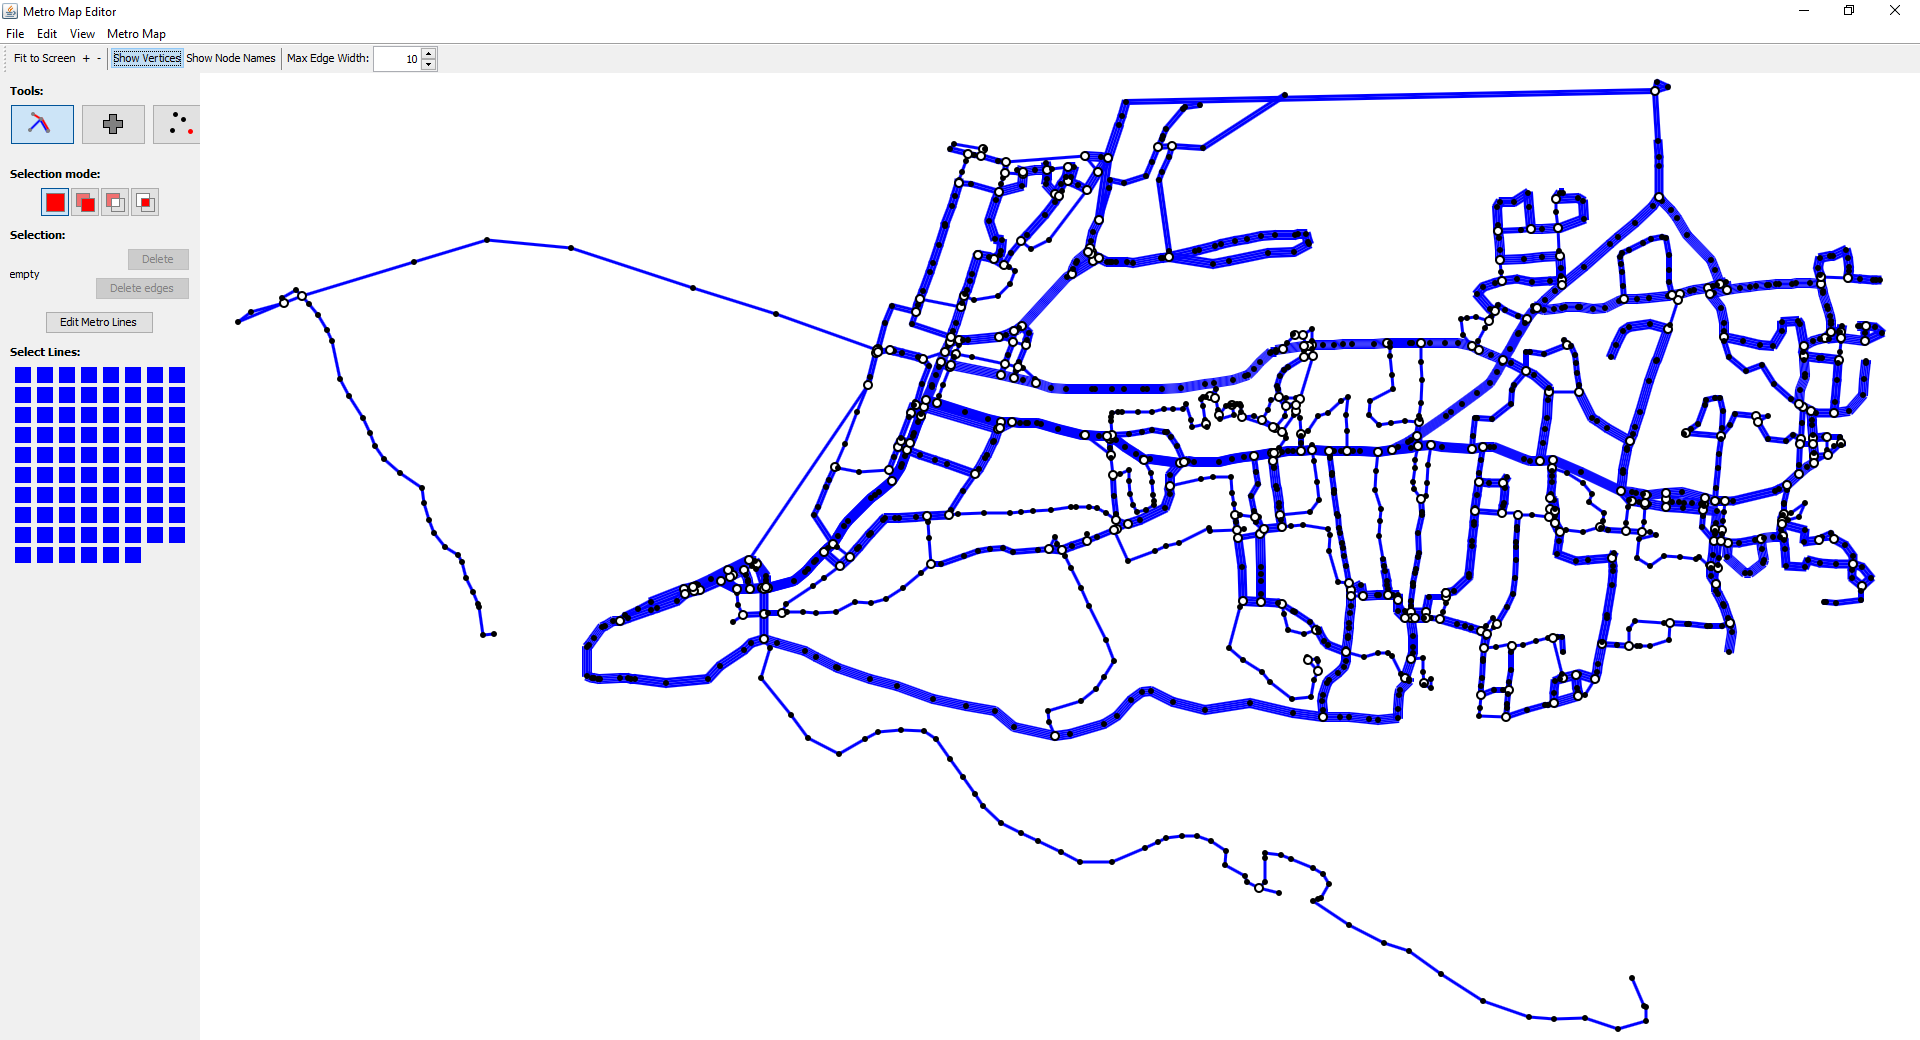
\includegraphics[width=\linewidth, trim=160 2 20 62, clip]{imagens/analiseMapas/inicial_azul.png}
    \caption{Bacia Norte / Nordeste (Azul): traçado geográfico de referência.}
    \label{fig:azul_inicial}
\end{figure}

\begin{figure}[H]
    \centering
    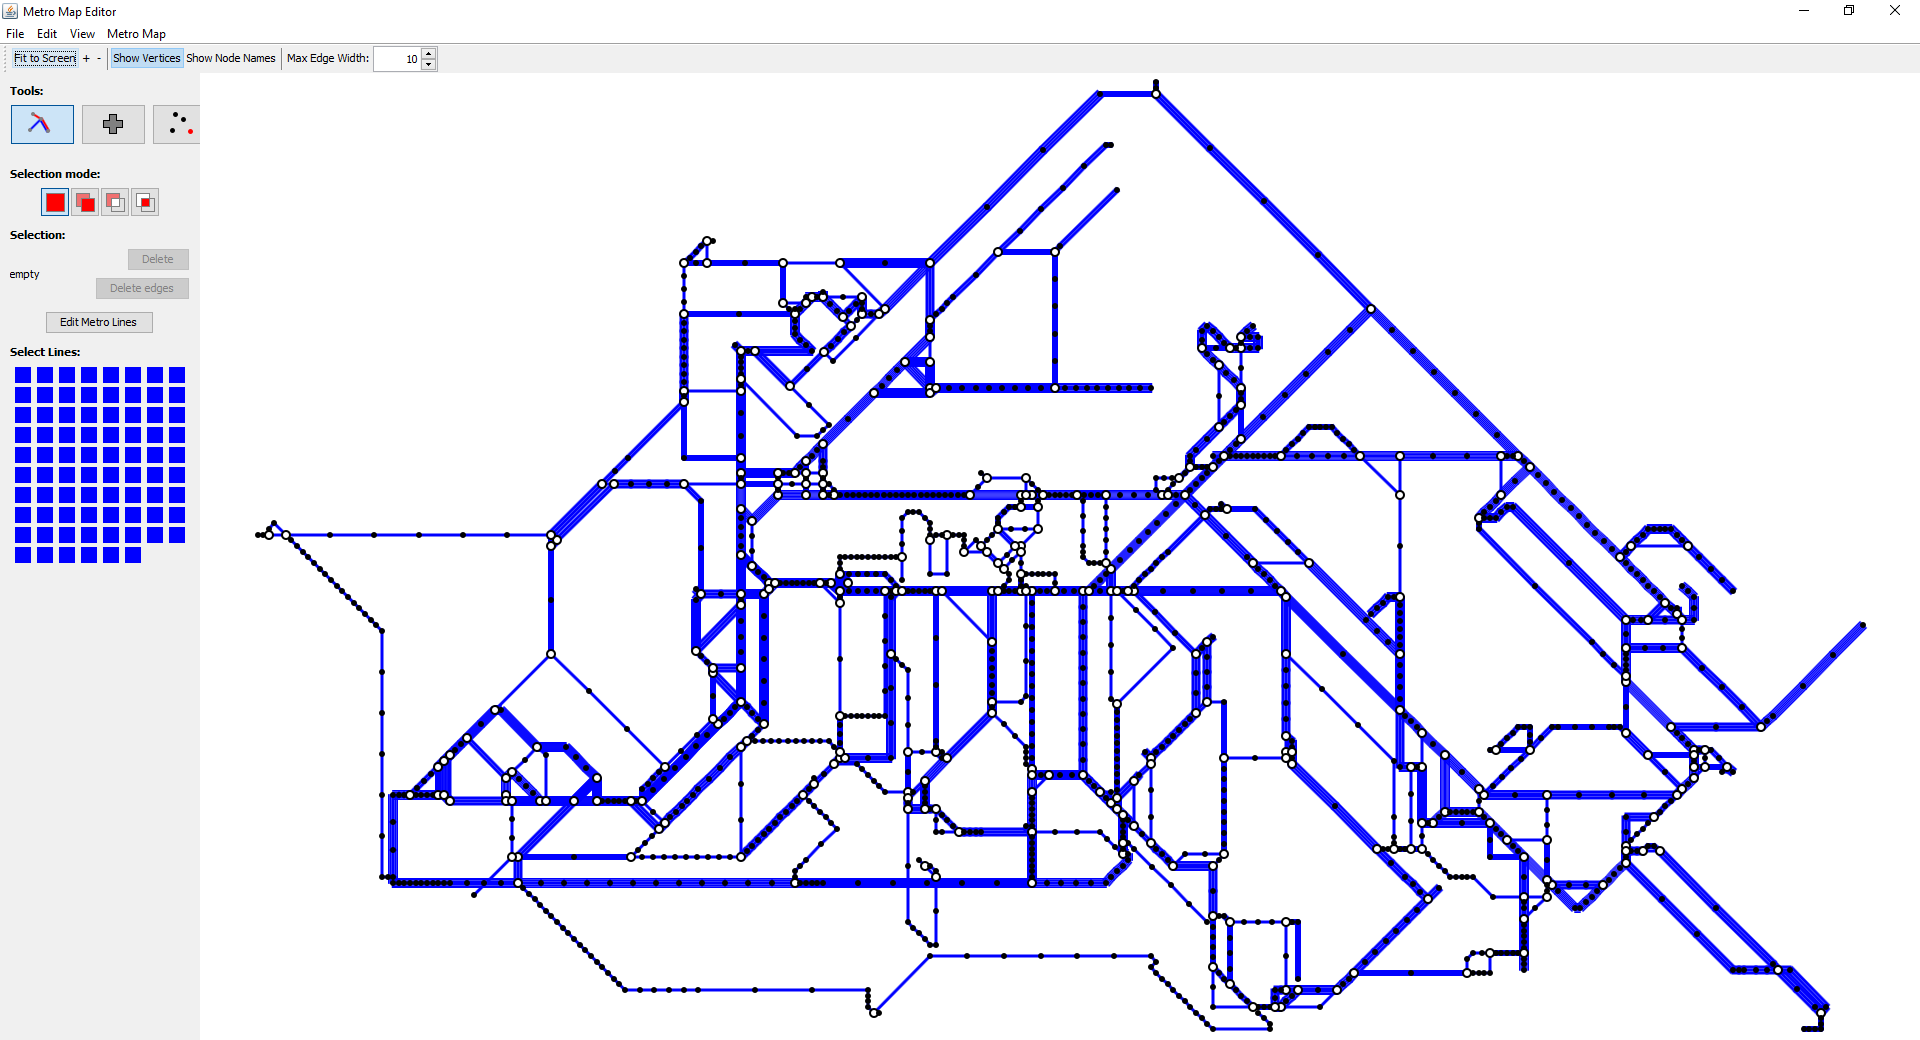
\includegraphics[width=\linewidth, trim=160 2 20 62, clip]{imagens/analiseMapas/biobjetiva_azul.png}
    \caption{Bacia Norte / Nordeste (Azul): esquematização biobjetiva (\textit{MIP Gap} = $20\%$).}
    \label{fig:azul_biobjetiva}
\end{figure}

\begin{figure}[H]
    \centering
    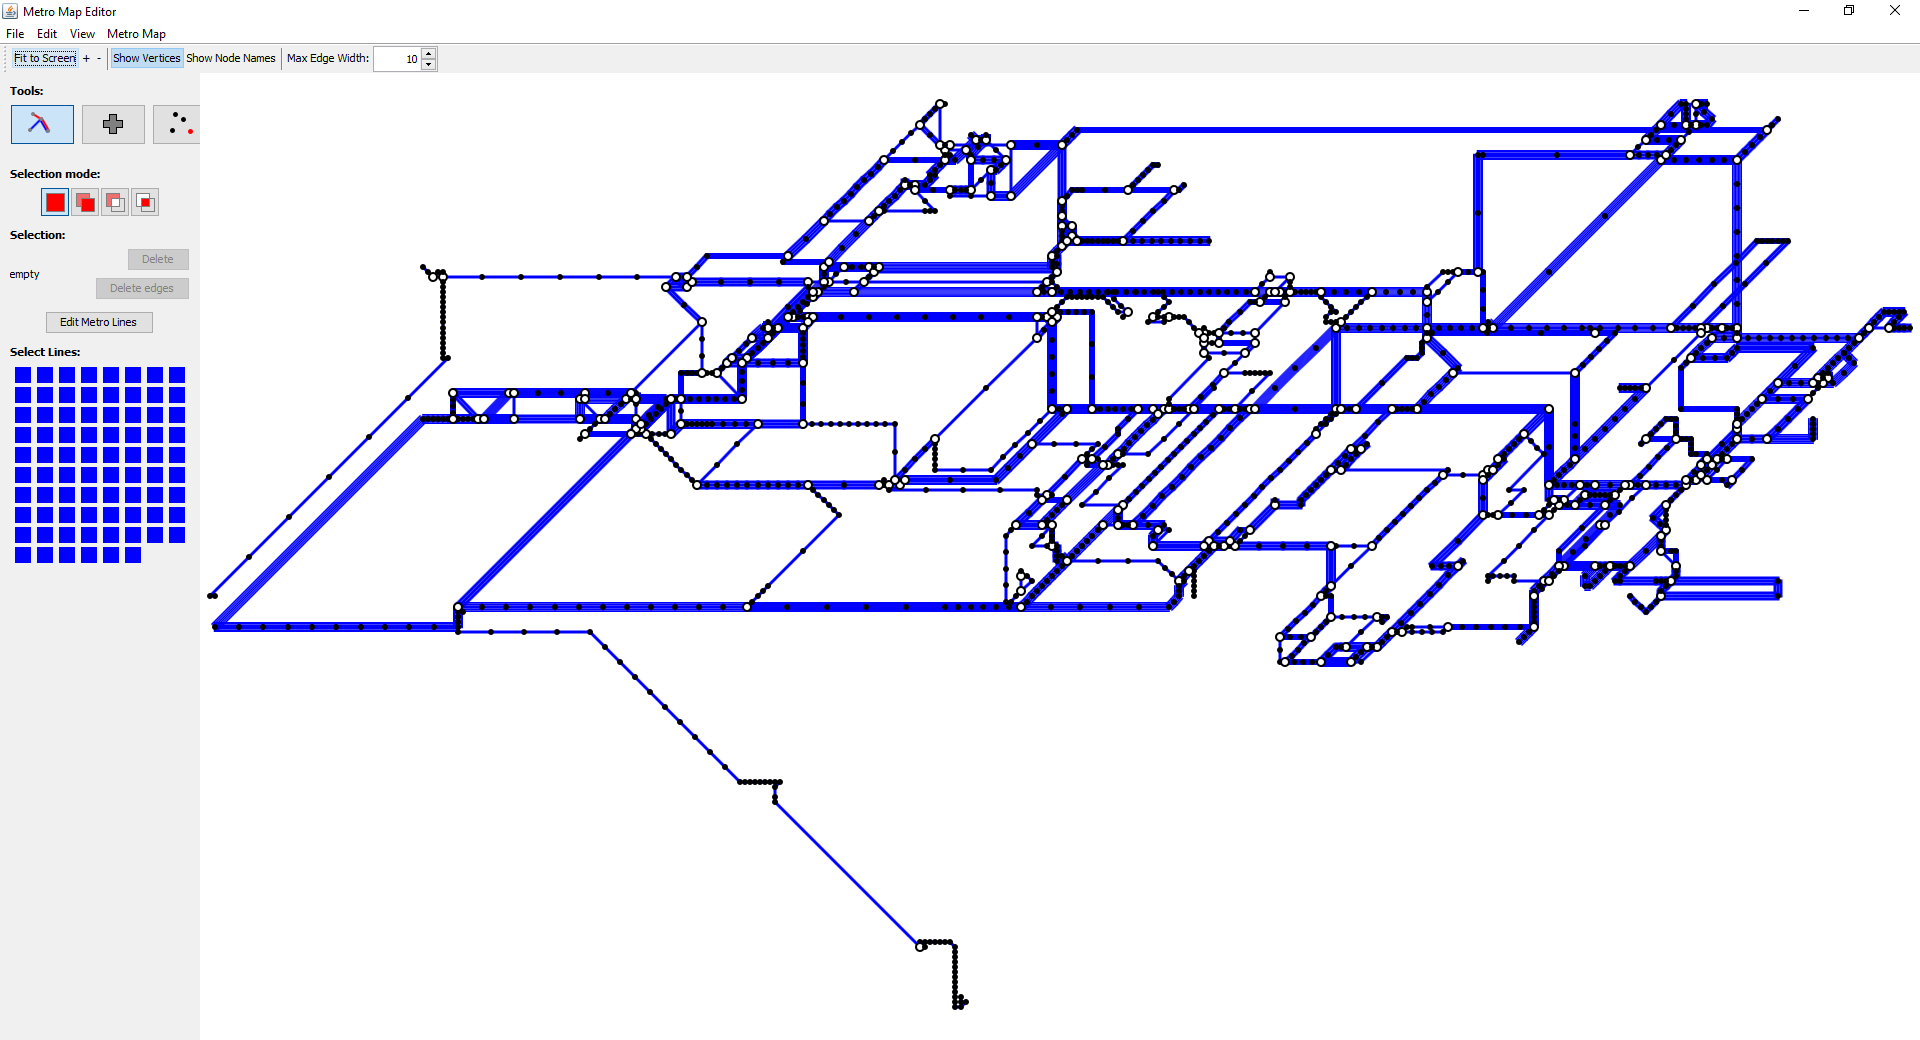
\includegraphics[width=\linewidth, trim=152 2 20 62, clip]{imagens/analiseMapas/triobjetiva_azul.png}
    \caption{Bacia Norte / Nordeste (Azul): esquematização triobjetiva (\textit{MIP Gap} = $60\%$).}
    \label{fig:azul_triobjetiva}
\end{figure}

Na Bacia Norte / Nordeste (Figuras~\ref{fig:azul_inicial}, \ref{fig:azul_biobjetiva} e \ref{fig:azul_triobjetiva}), observa-se claramente o efeito da calibração de $L_{\max} = 10$. Por incorporar itinerários expressos (linhas SD72 e SD73) caracterizados por arestas substancialmente extensas no extremo norte da rede, a utilização da cota máxima convencional ($L_{\max} = 4$) tornava o modelo matemático inviável. No comparativo entre as formulações, a variante triobjetiva (Figura~\ref{fig:azul_triobjetiva}) destacou-se por preservar de forma mais equilibrada a proporção e a geometria global da malha em relação à biobjetiva (Figura~\ref{fig:azul_biobjetiva}); em contrapartida, a formulação biobjetiva foi superior na manutenção do alinhamento vertical das rotas no eixo norte-sul, as quais sofreram inclinações diagonais na solução triobjetiva.

\begin{figure}[H]
    \centering
    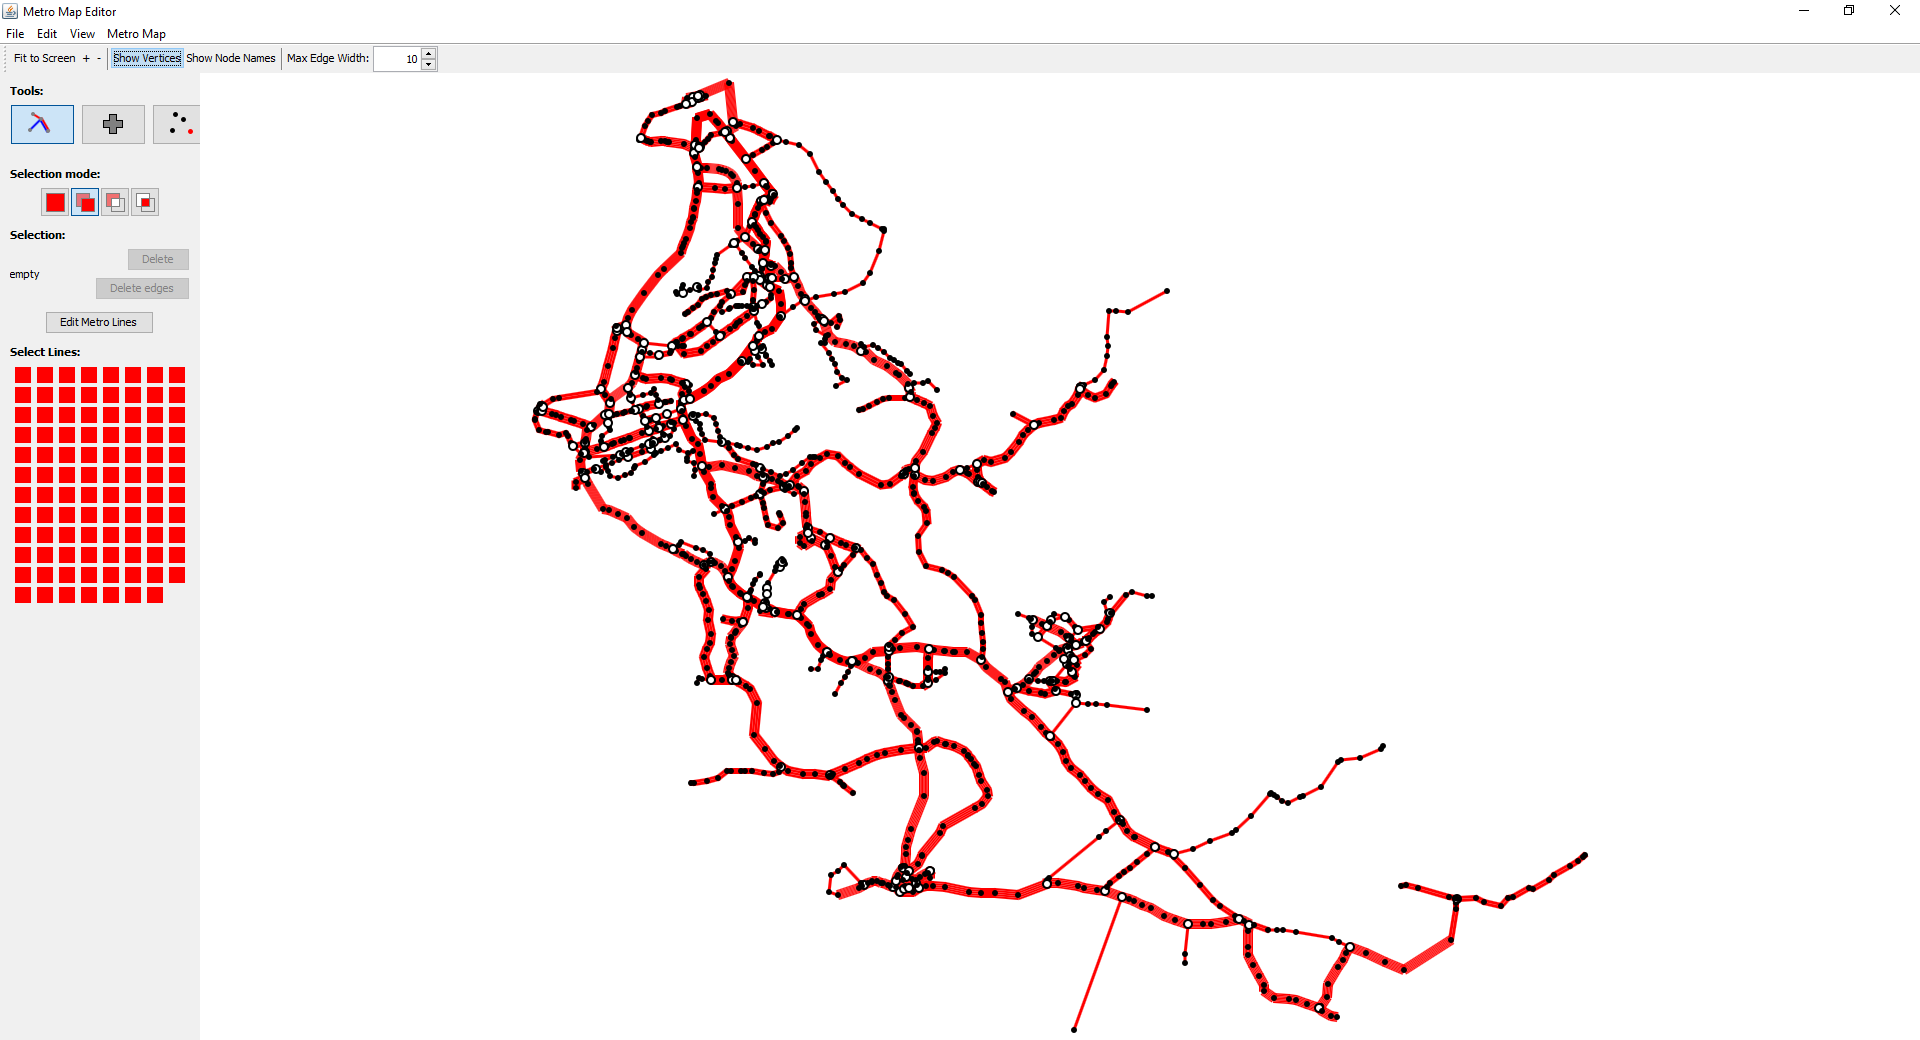
\includegraphics[width=\linewidth, trim=160 2 20 56, clip]{imagens/analiseMapas/inicial_vermelho.png}
    \caption{Bacia Sul (Vermelha): traçado geográfico de referência.}
    \label{fig:vermelho_inicial}
\end{figure}

\begin{figure}[H]
    \centering
    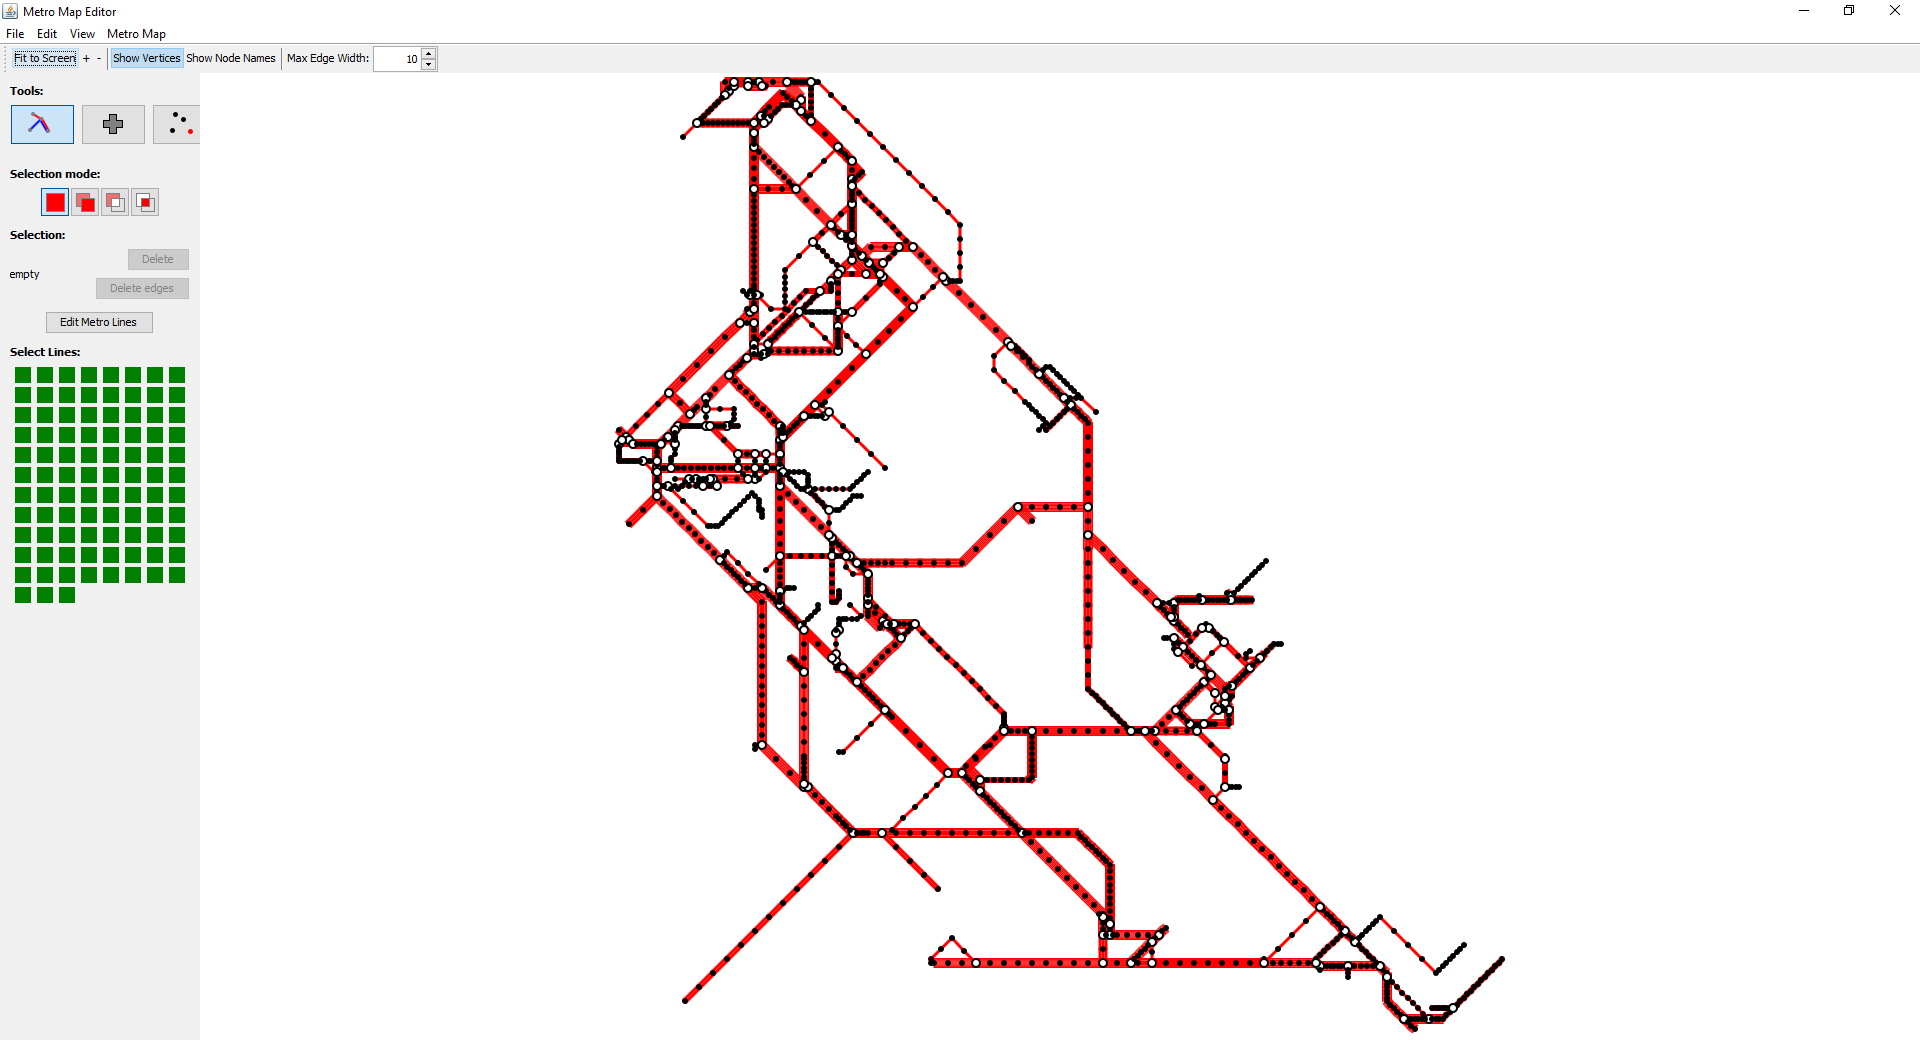
\includegraphics[width=\linewidth, trim=160 2 20 56, clip]{imagens/analiseMapas/biobjetiva_vermelho.png}
    \caption{Bacia Sul (Vermelha): esquematização biobjetiva (\textit{MIP Gap} = $10\%$).}
    \label{fig:vermelho_biobjetiva}
\end{figure}

\begin{figure}[H]
    \centering
    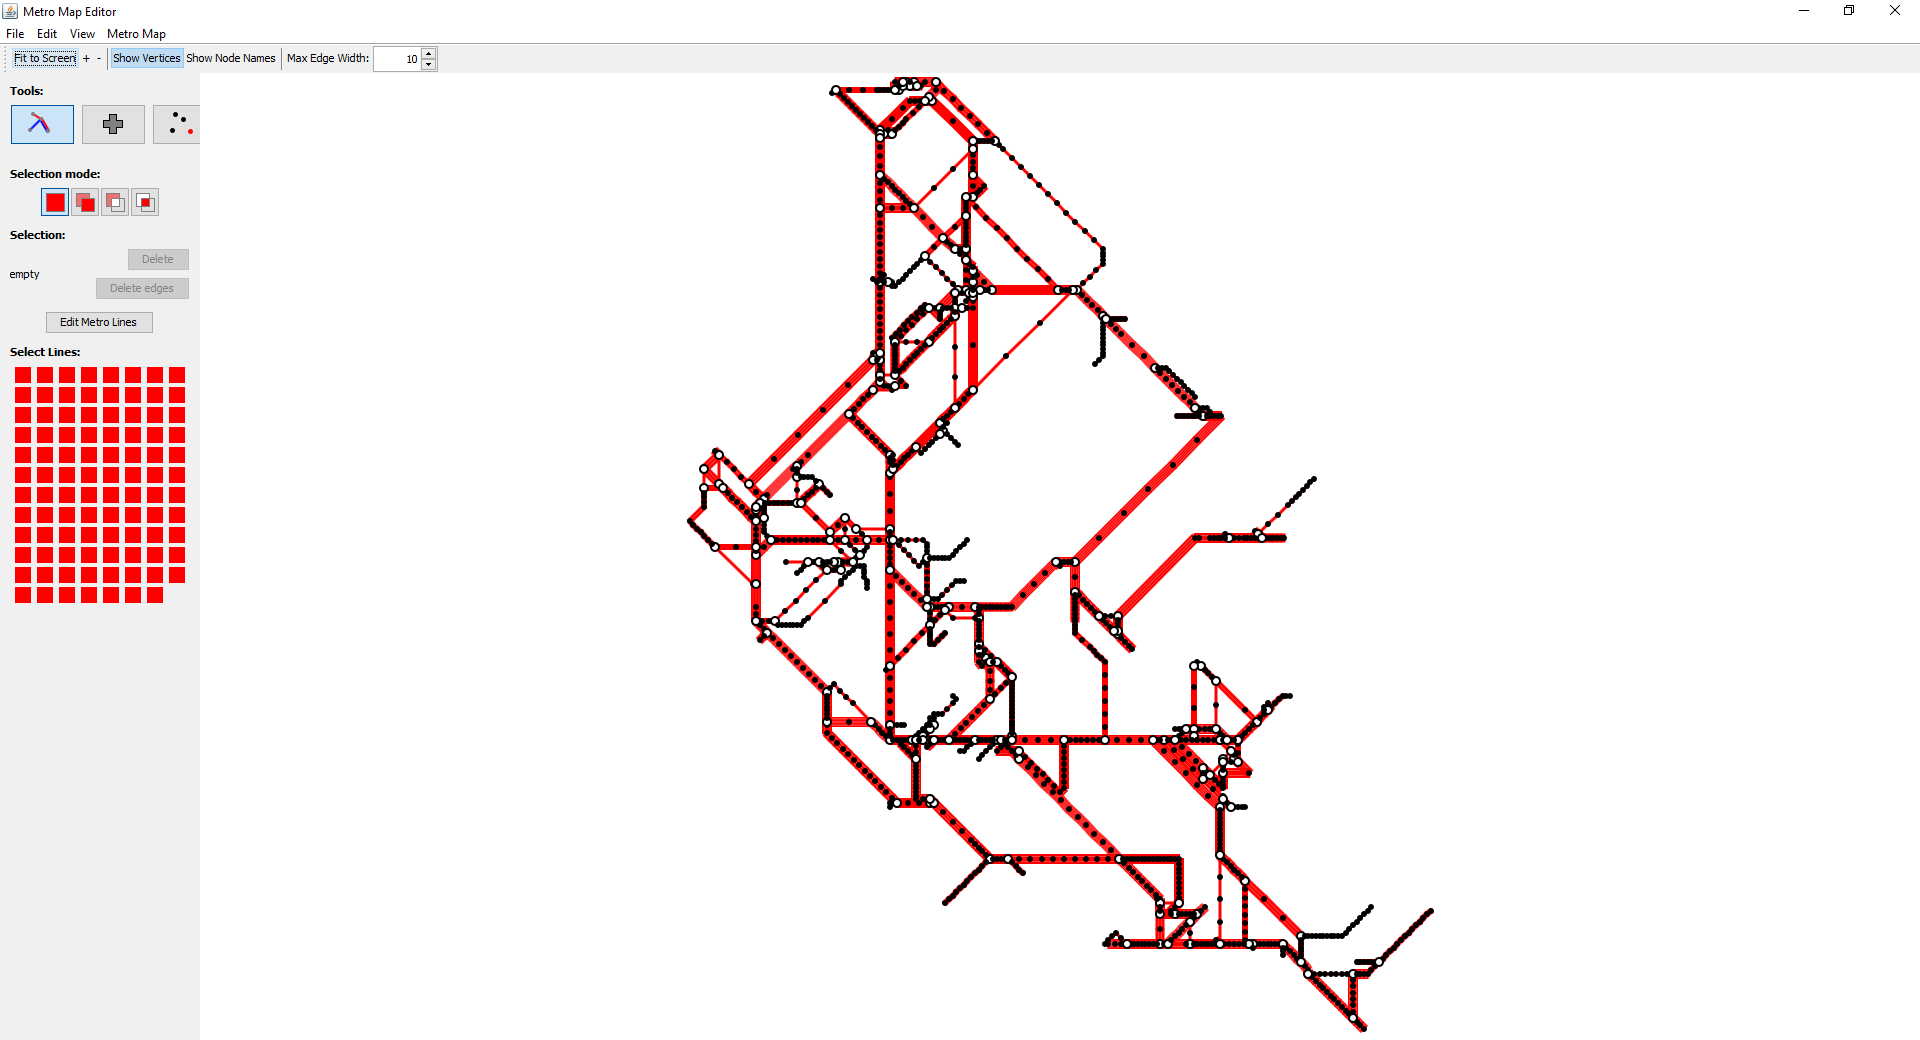
\includegraphics[width=\linewidth, trim=160 2 20 56, clip]{imagens/analiseMapas/triobjetiva_vermelho.png}
    \caption{Bacia Sul (Vermelha): esquematização triobjetiva (\textit{MIP Gap} = $30\%$).}
    \label{fig:vermelho_triobjetiva}
\end{figure}

Para a Bacia Sul (Figuras~\ref{fig:vermelho_inicial}, \ref{fig:vermelho_biobjetiva} e \ref{fig:vermelho_triobjetiva}), ambos os modelos produziram soluções convergentes e consistentes entre si, sendo bem-sucedidos em preservar a estrutura topológica global e a orientação dos principais eixos viários da região. Contudo, nas áreas de maior densidade de vértices e interseções, a formulação triobjetiva apresentou maior dificuldade para organizar os elementos de forma plenamente legível, enquanto a versão biobjetiva manteve uma disposição espacial mais clara e desobstruída nesses trechos concorridos.

\begin{figure}[H]
    \centering
    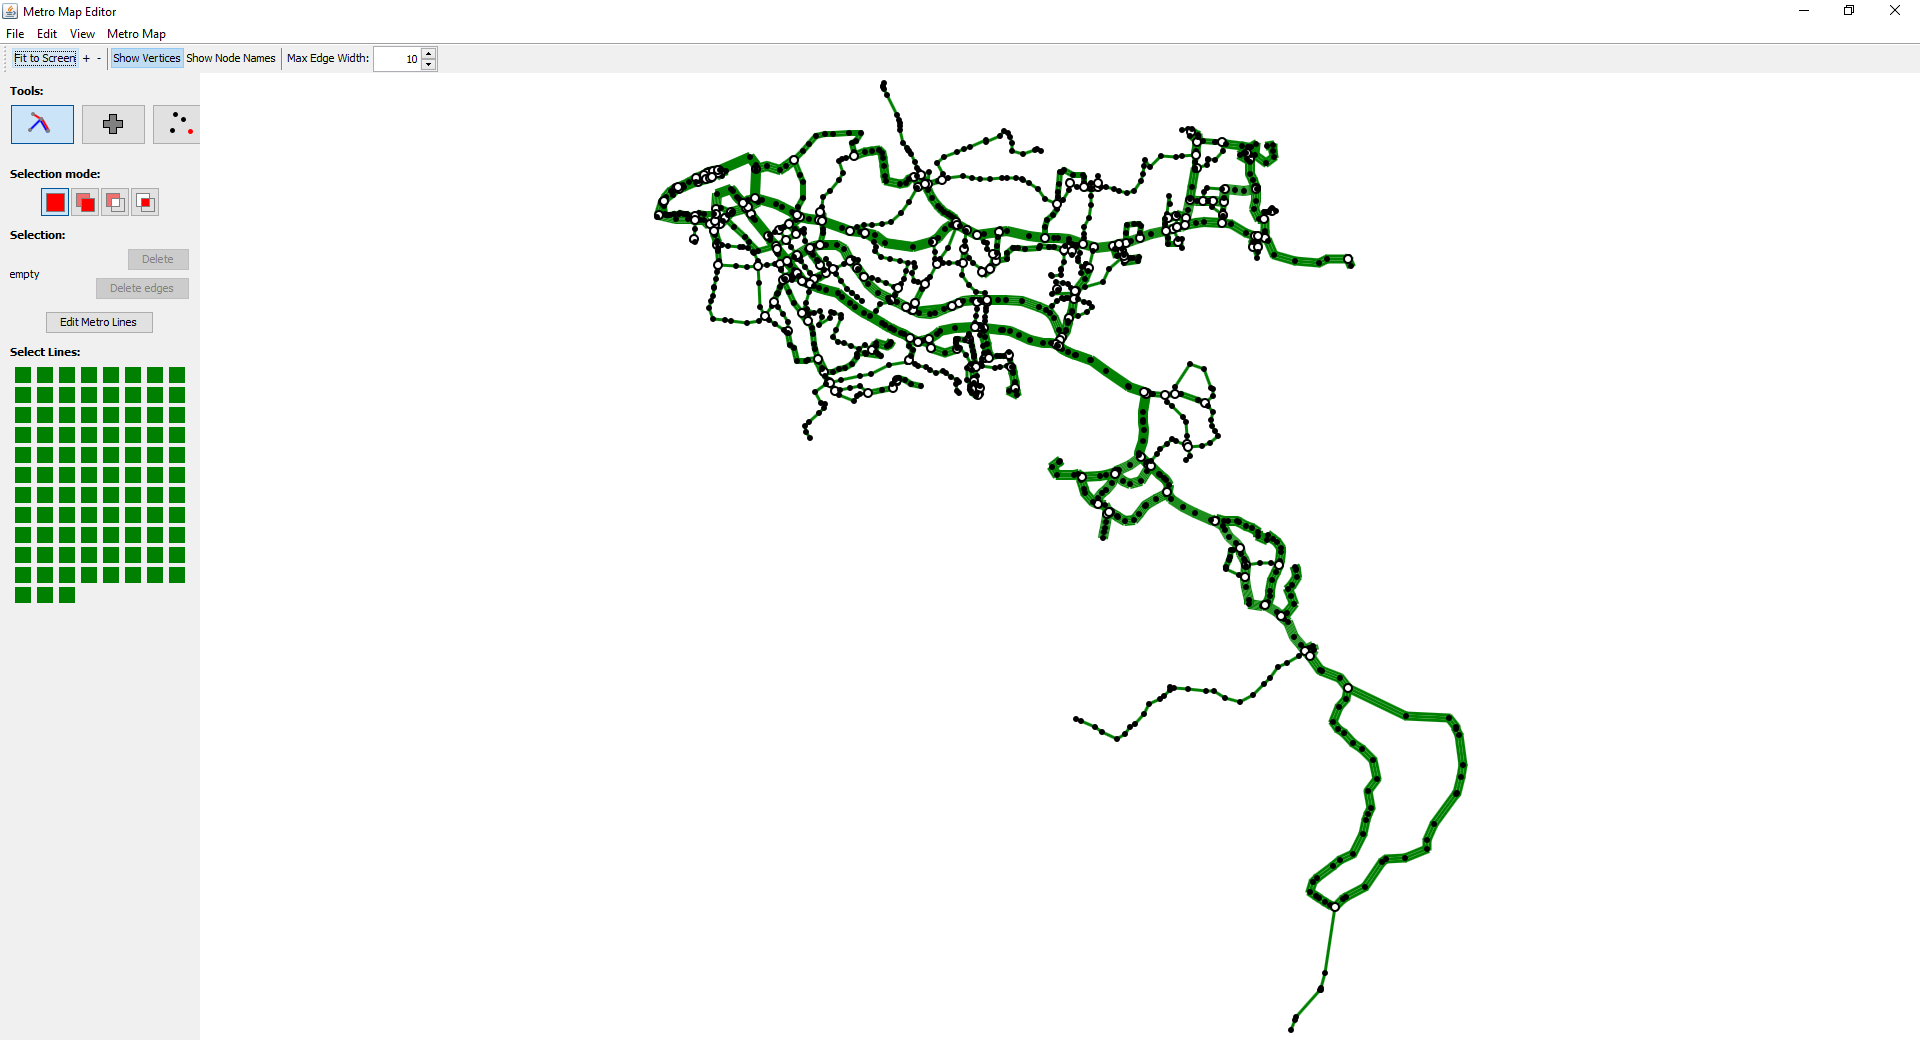
\includegraphics[width=\linewidth, trim=160 2 20 56, clip]{imagens/analiseMapas/inicial_verde.png}
    \caption{Bacia Leste / Sudeste (Verde): traçado geográfico de referência.}
    \label{fig:verde_inicial}
\end{figure}

\begin{figure}[H]
    \centering
    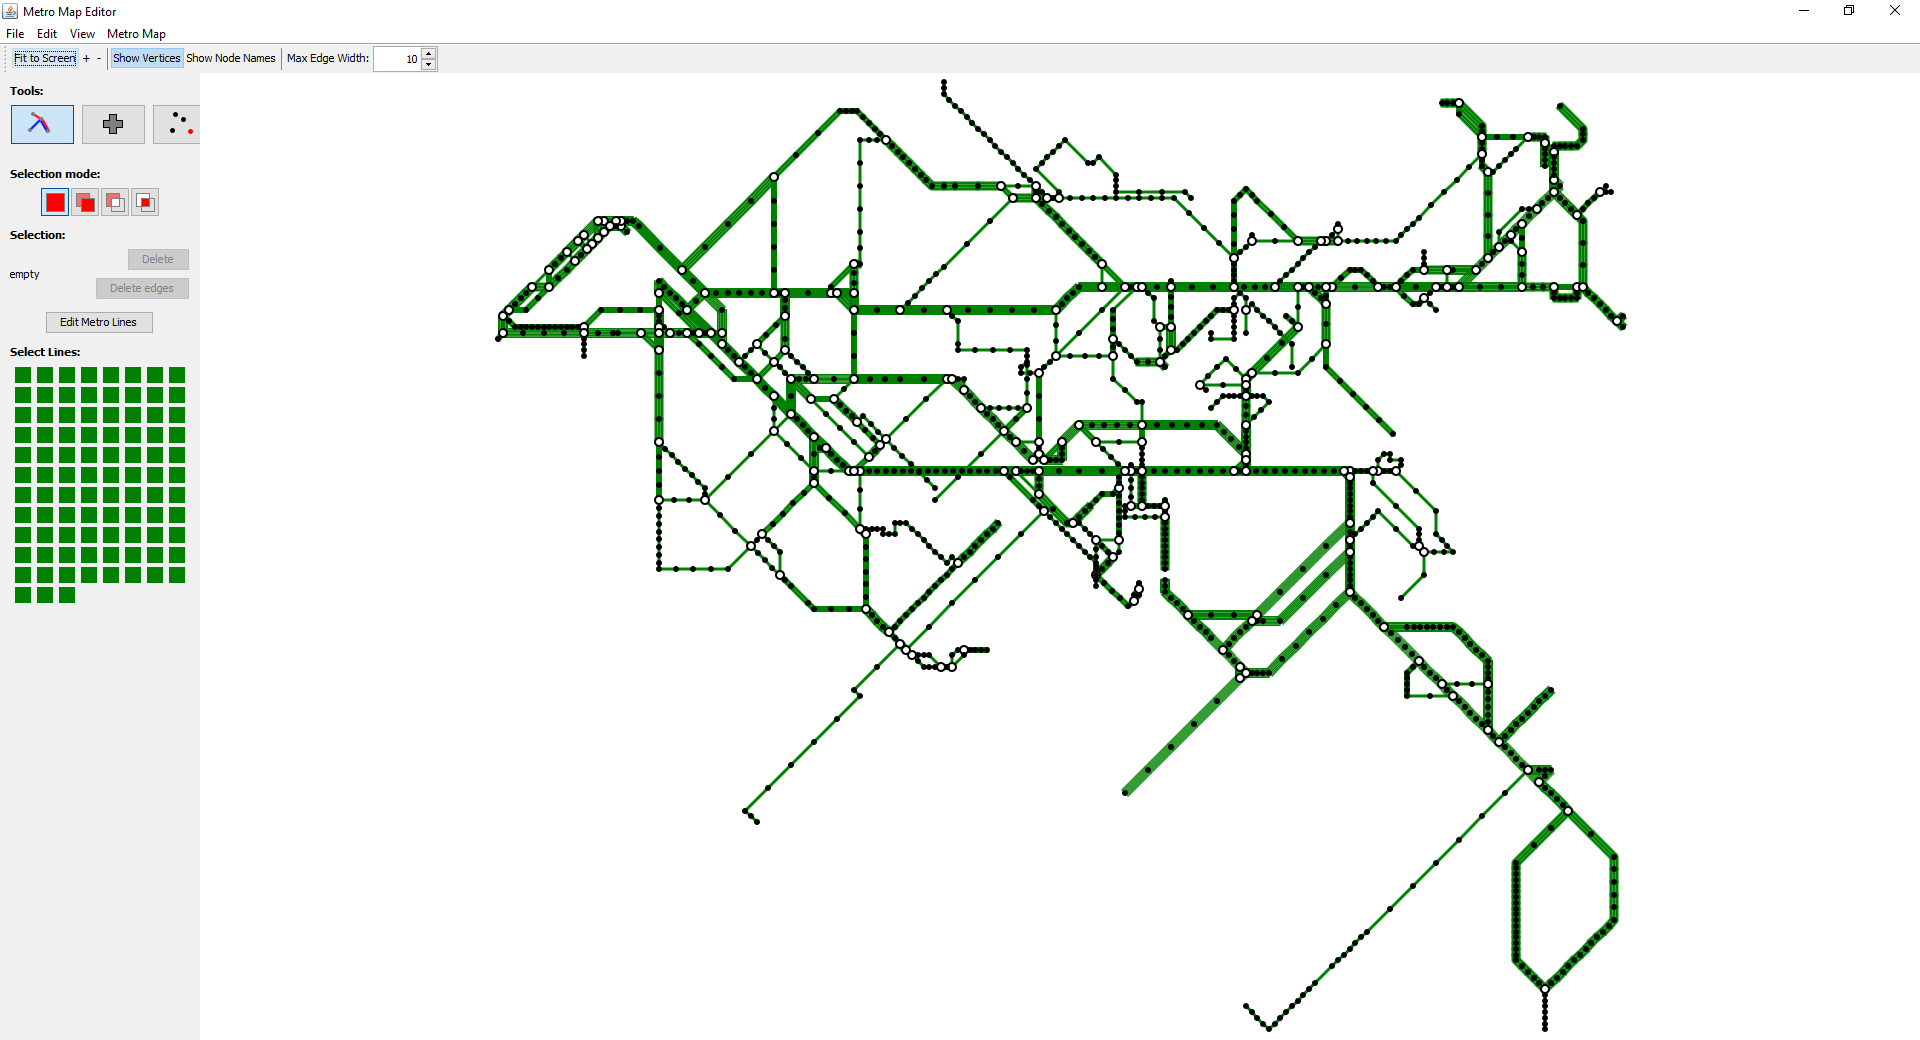
\includegraphics[width=\linewidth, trim=160 2 20 56, clip]{imagens/analiseMapas/biobjetiva_verde.png}
    \caption{Bacia Leste / Sudeste (Verde): esquematização biobjetiva (\textit{MIP Gap} = $10\%$).}
    \label{fig:verde_biobjetiva}
\end{figure}

\begin{figure}[H]
    \centering
    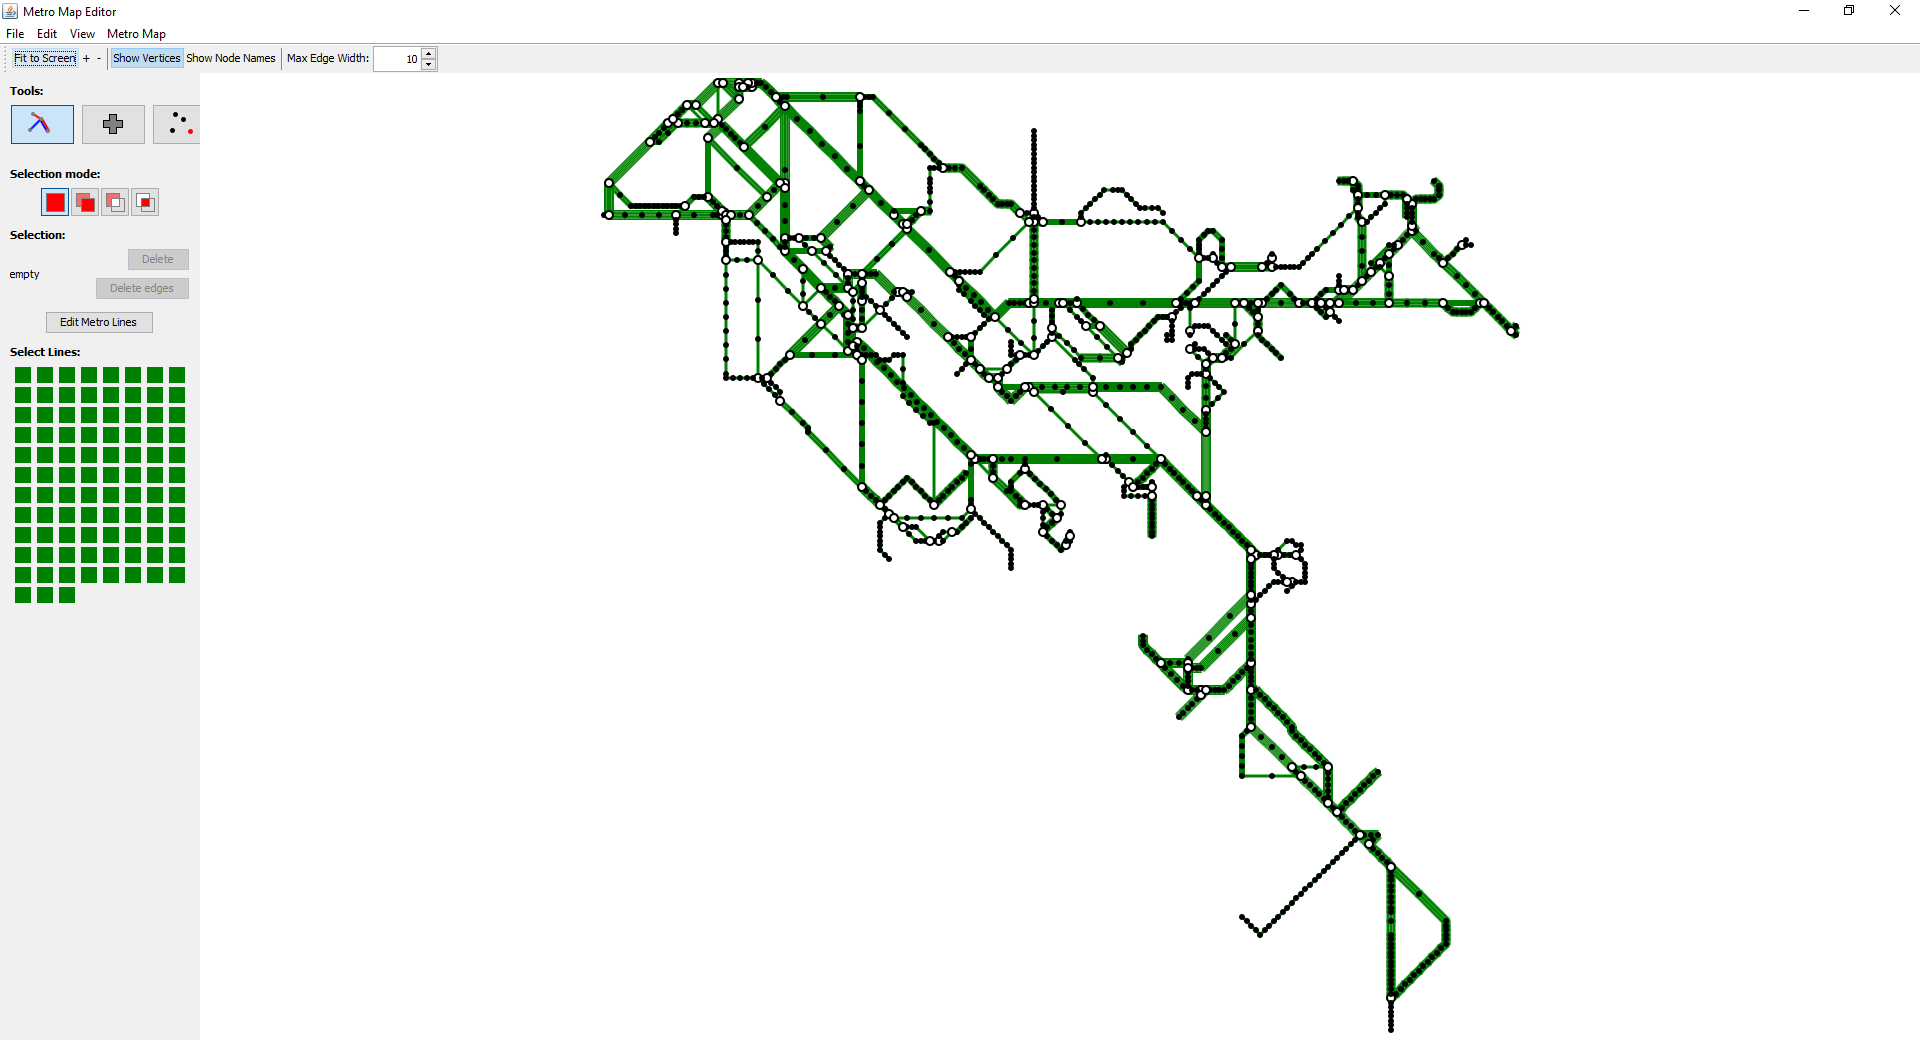
\includegraphics[width=\linewidth, trim=160 2 20 56, clip]{imagens/analiseMapas/triobjetiva_verde.png}
    \caption{Bacia Leste / Sudeste (Verde): esquematização triobjetiva (\textit{MIP Gap} = $30\%$).}
    \label{fig:verde_triobjetiva}
\end{figure}

Na Bacia Leste / Sudeste (Figuras~\ref{fig:verde_inicial}, \ref{fig:verde_biobjetiva} e \ref{fig:verde_triobjetiva}), a versão triobjetiva preservou com maior fidelidade a geometria global e as proporções da malha original. Em contraste, a formulação biobjetiva causou uma compressão vertical acentuada no mapa e estendeu excessivamente certas arestas terminais nas extremidades das rotas, resultando em uma silhueta que dificulta o reconhecimento imediato do traçado frente à sua geometria geográfica de referência.

\begin{figure}[H]
    \centering
    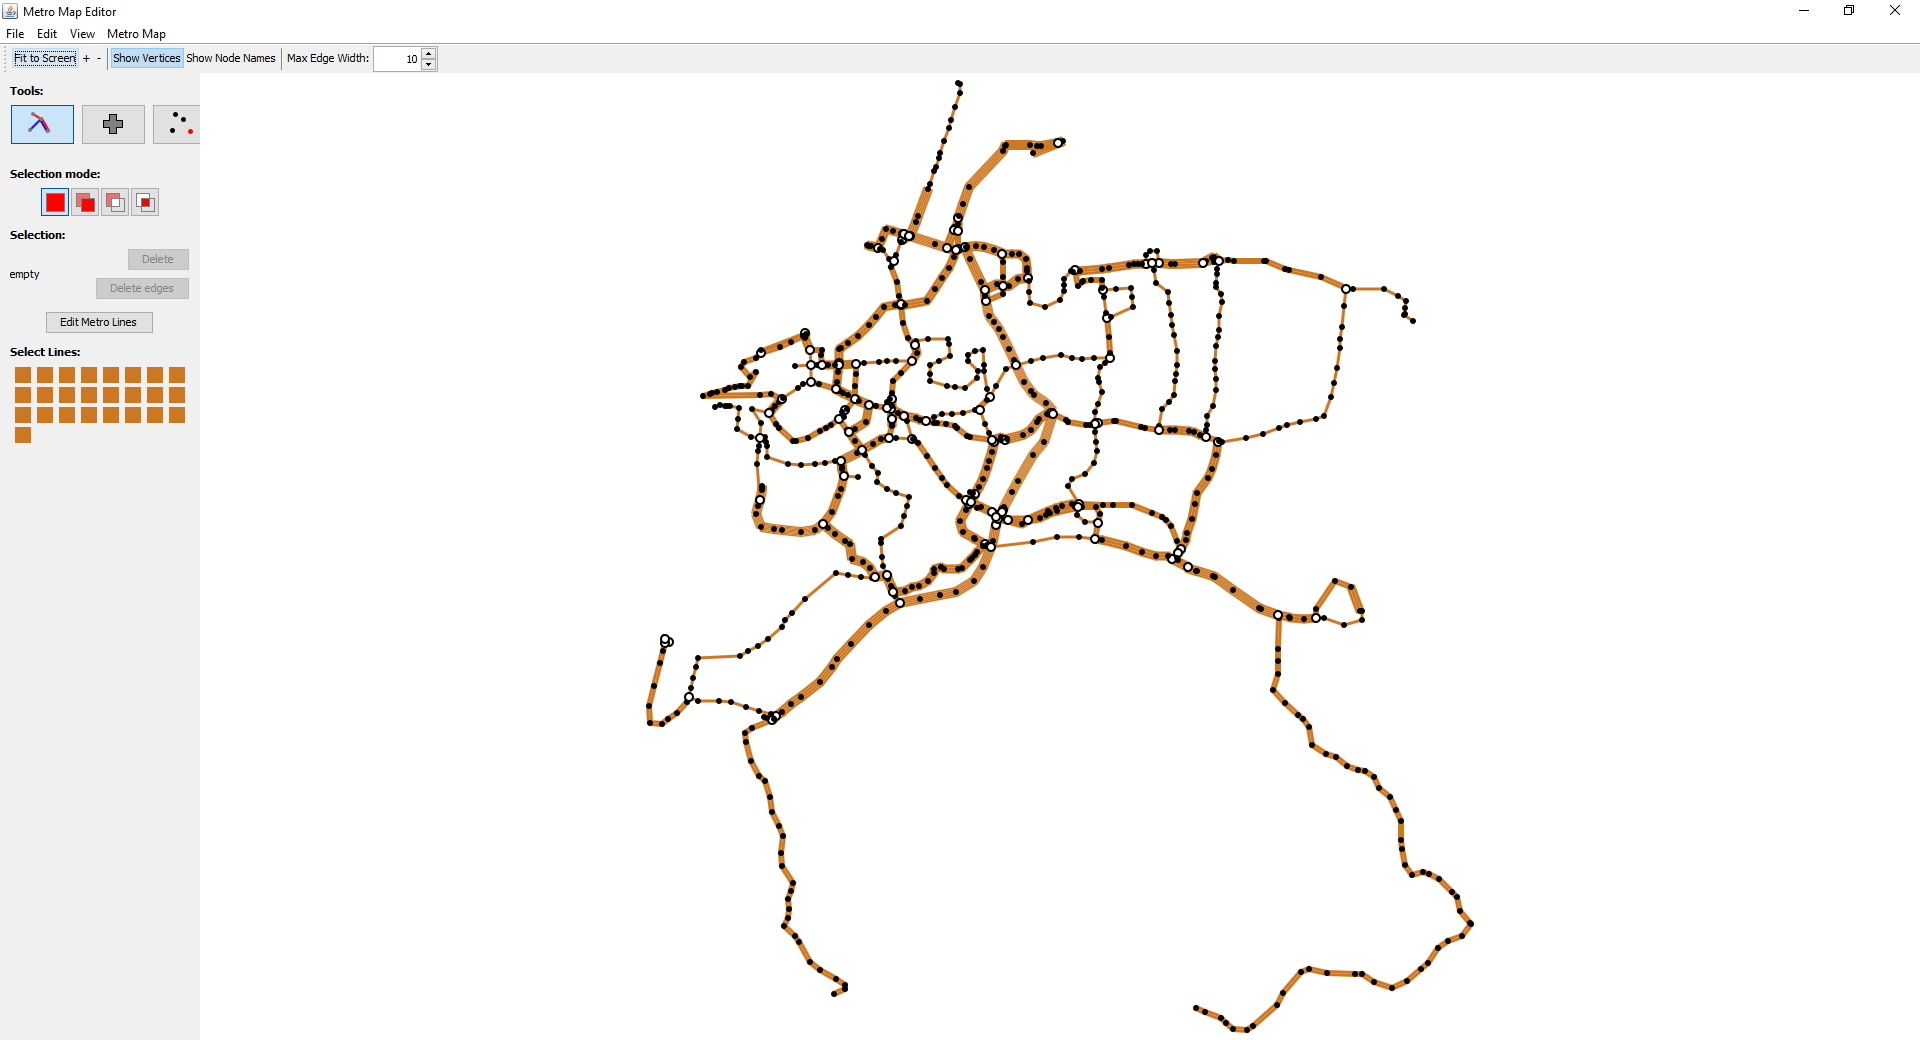
\includegraphics[width=\linewidth, trim=160 2 20 56, clip]{imagens/analiseMapas/inicial_laranja.png}
    \caption{Linhas Transversais e Circulares (Laranja): traçado geográfico de referência.}
    \label{fig:laranja_inicial}
\end{figure}

\begin{figure}[H]
    \centering
    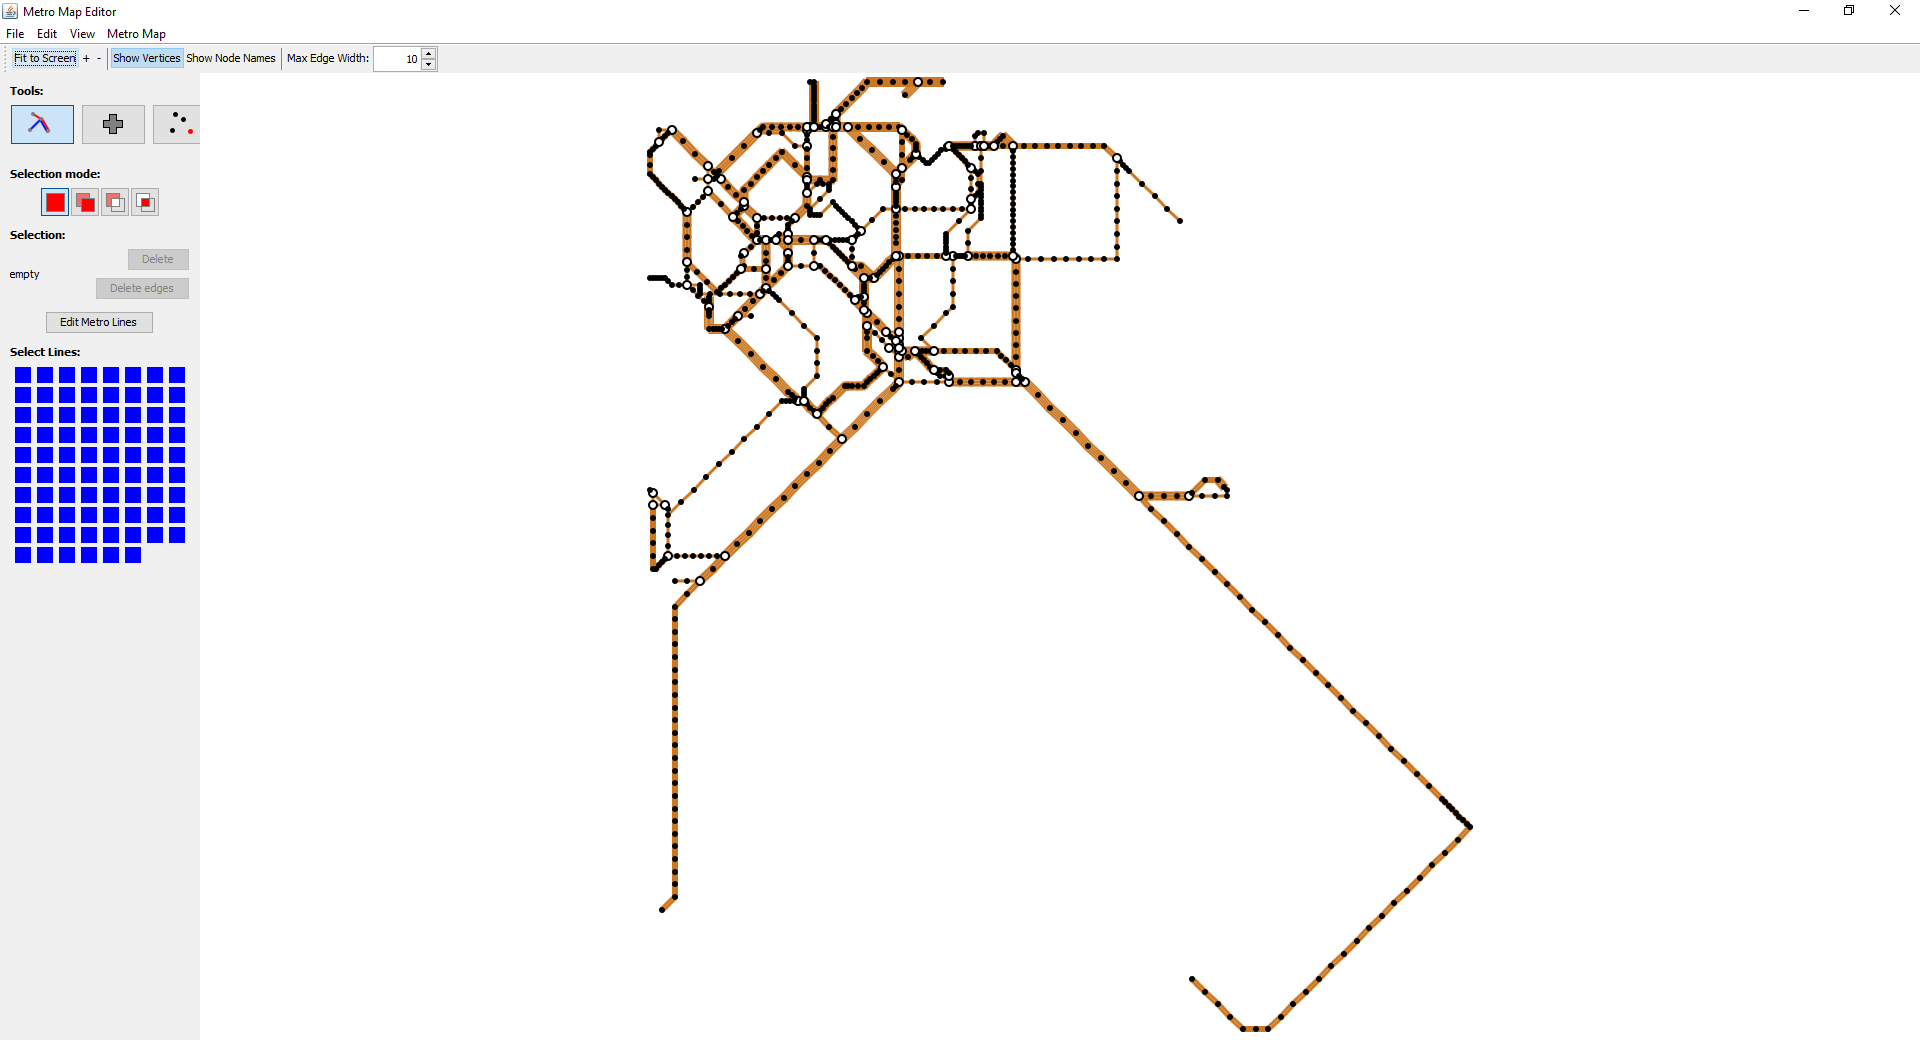
\includegraphics[width=\linewidth, trim=160 2 20 56, clip]{imagens/analiseMapas/biobjetiva_laranja.png}
    \caption{Linhas Transversais e Circulares (Laranja): esquematização biobjetiva (\textit{MIP Gap} = $10\%$).}
    \label{fig:laranja_biobjetiva}
\end{figure}

\begin{figure}[H]
    \centering
    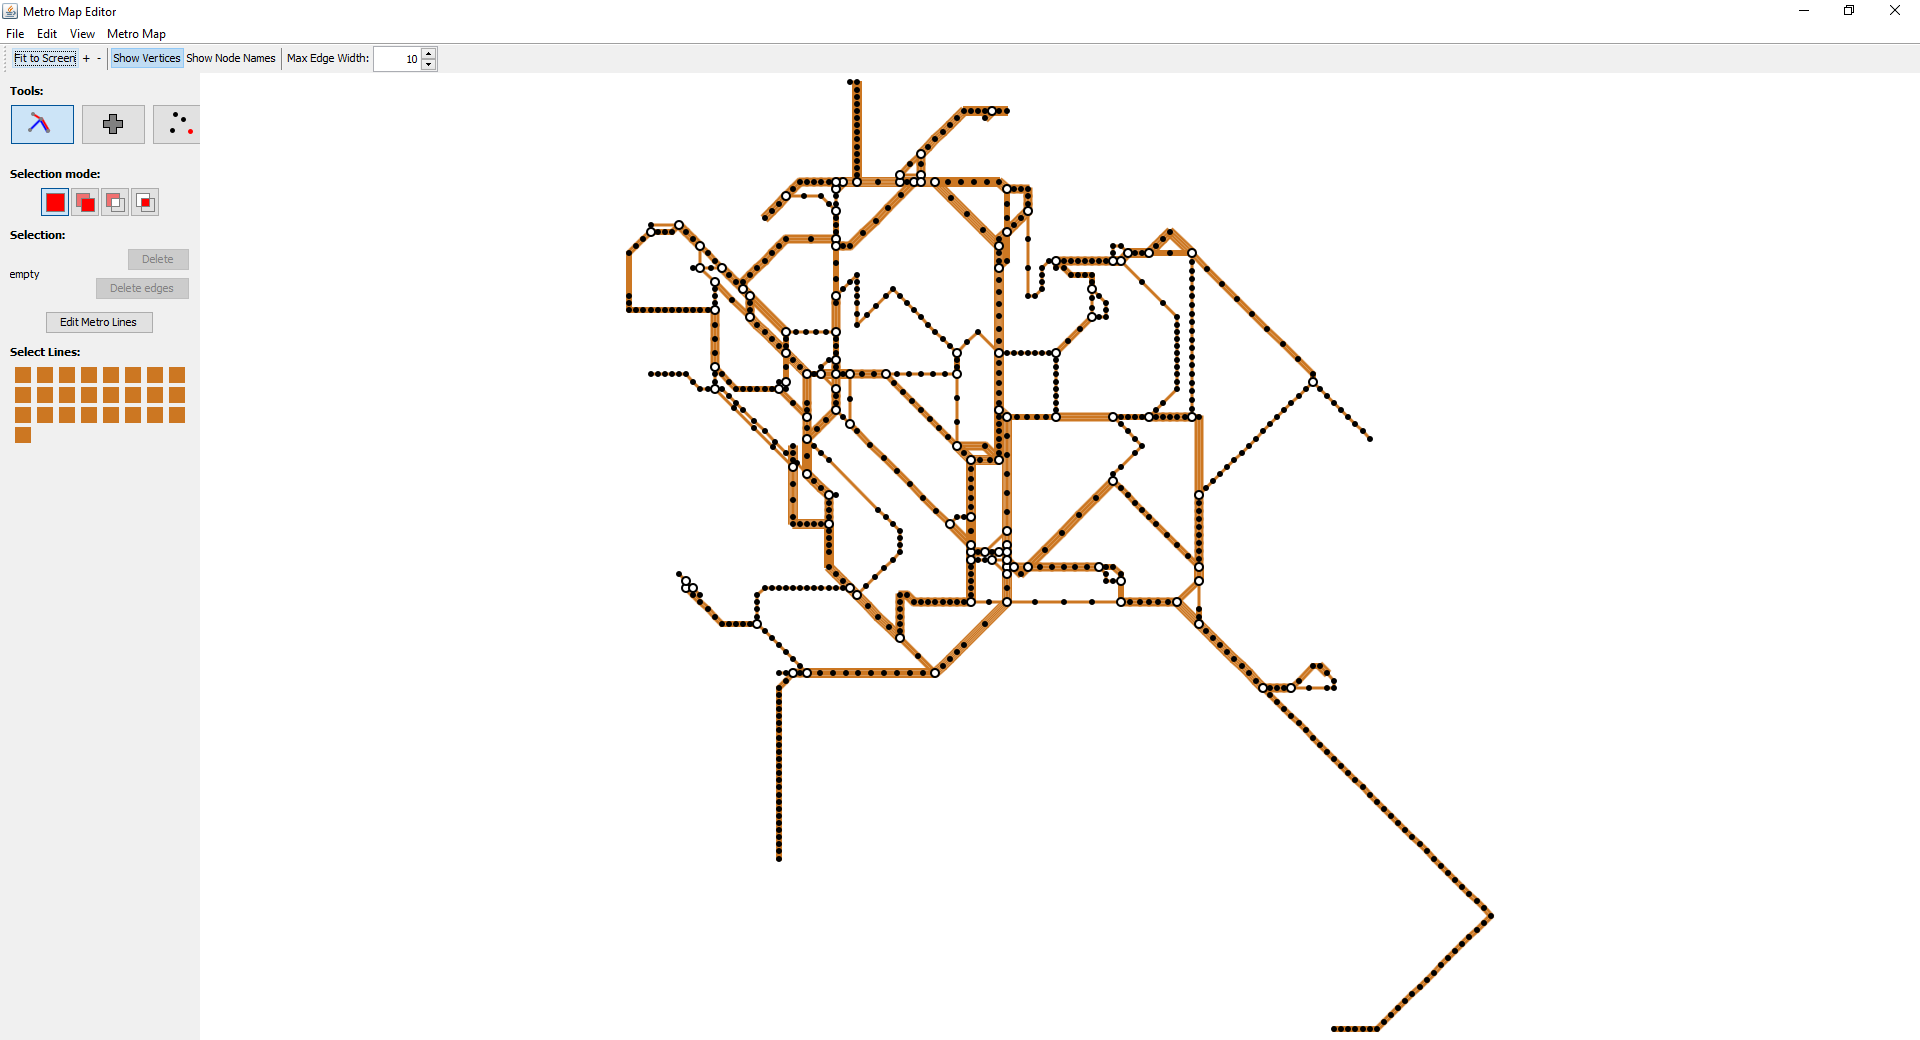
\includegraphics[width=\linewidth, trim=160 2 20 56, clip]{imagens/analiseMapas/triobjetiva_laranja.png}
    \caption{Linhas Transversais e Circulares (Laranja): esquematização triobjetiva (\textit{MIP Gap} = $20\%$).}
    \label{fig:laranja_triobjetiva}
\end{figure}

No subsistema das Linhas Transversais e Circulares (Figuras~\ref{fig:laranja_inicial}, \ref{fig:laranja_biobjetiva} e \ref{fig:laranja_triobjetiva}), ambas as formulações também apresentaram resultados bastante similares. Por se tratar de um recorte viário de topologia relativamente menos complexa, nenhuma das abordagens se sobressaiu visualmente em relação à outra, residindo a principal diferença prática no fato de que a variante triobjetiva promoveu uma maior compressão no comprimento das arestas em comparação à biobjetiva.

A fim de verificar a consistência das proporções dos mapas esquemáticos resultantes em relação à geografia original da rede viária, realizou-se uma avaliação das dimensões espaciais ocupadas pelos grafos gerados. Conforme detalhado na Seção~\ref{subsec:parametros_solver}, o posicionamento dos vértices no modelo MIP é delimitado por uma grade discreta, com largura $\text{GRID\_WIDTH} = |V|$ e altura $\text{GRID\_HEIGHT} = \lfloor |V| \times r_{\text{geo}} \rfloor$, onde $r_{\text{geo}} = (\text{lat}_{\max} - \text{lat}_{\min}) / (\text{lon}_{\max} - \text{lon}_{\min})$ denota a razão de aspecto geográfica da malha sob análise. Além de delimitar o domínio das variáveis de coordenadas ($0 \le x(v) \le \text{GRID\_WIDTH}$ e $0 \le y(v) \le \text{GRID\_HEIGHT}$ para todo $v \in V$), tal configuração condiciona diretamente a magnitude da constante Big-$M$, definida como $M = 10{,}0 + \max(\text{GRID\_WIDTH}, \text{GRID\_HEIGHT})$, parâmetro crucial utilizado para desativar restrições lineares disjuntivas.

Com o intuito de caracterizar o comportamento espacial das soluções, extraiu-se a caixa delimitadora mínima (\textit{bounding box}) que circunscreve o conjunto de vértices de cada bacia operacional após a otimização, sob as formulações biobjetiva e triobjetiva. Esse procedimento permite mensurar as proporções tomadas no plano cartesiano discreto e verificar em que medida o solucionador utilizou o espaço disponibilizado na grade. A Tabela~\ref{tab:bounding_box} sintetiza esses resultados, reunindo as dimensões nominais da grade de entrada, as coordenadas extremas ocupadas pelos nós ($X_{\min}, X_{\max}, Y_{\min}, Y_{\max}$), a extensão linear em cada eixo ($\Delta X = X_{\max} - X_{\min}$ e $\Delta Y = Y_{\max} - Y_{\min}$) e a correspondente taxa de ocupação da área total. Adicionalmente, apresenta-se a razão de aspecto resultante do layout ($r_{\text{layout}} = \Delta Y / \Delta X$) confrontada com a proporção geográfica de referência ($r_{\text{geo}}$), quantificando-se o desvio relativo percentual entre a geometria esquematizada e o traçado real.

\begin{table}[H]
    \centering
    \caption{Dimensões da grade, caixas delimitadoras (\textit{bounding boxes}) e taxas de ocupação espacial por bacia operacional.}
    \label{tab:bounding_box}
    \resizebox{\linewidth}{!}{%
    \begin{tabular}{llcccccccc}
        \toprule
        \textbf{Bacia Operacional} & \textbf{Formulação} & \textbf{Grade Fornecida} & \textbf{$r_{\text{geo}}$} & \textbf{Extensão $X$} & \textbf{Extensão $Y$} & \textbf{Área Útil} & \textbf{Ocup. Área} & \textbf{$r_{\text{layout}}$} & \textbf{Desvio $r$} \\
        \midrule
        \multirow{2}{*}{Norte / Nordeste (Azul)} 
            & Biobjetiva  & \multirow{2}{*}{$588 \times 339$} & \multirow{2}{*}{0,576} & $[0, 284]$ & $[0, 167]$ & $284 \times 167$ & 23,8\% & 0,588 & \textbf{+2,0\%} \\
            & Triobjetiva &                                   &                        & $[0, 335]$ & $[0, 178]$ & $335 \times 178$ & 29,9\% & 0,531 & -7,8\% \\
        \midrule
        \multirow{2}{*}{Sul (Vermelha)} 
            & Biobjetiva  & \multirow{2}{*}{$480 \times 428$} & \multirow{2}{*}{0,892} & $[0, 252]$ & $[0, 270]$ & $252 \times 270$ & 33,1\% & 1,071 & +20,1\% \\
            & Triobjetiva &                                   &                        & $[0, 204]$ & $[172, 428]$ & $204 \times 256$ & 25,4\% & 1,255 & +40,7\% \\
        \midrule
        \multirow{2}{*}{Leste / Sudeste (Verde)} 
            & Biobjetiva  & \multirow{2}{*}{$522 \times 614$} & \multirow{2}{*}{1,176} & $[0, 195]$ & $[0, 164]$ & $195 \times 164$ & 10,0\% & 0,841 & -28,5\% \\
            & Triobjetiva &                                   &                        & $[321, 522]$ & $[405, 614]$ & $201 \times 209$ & 13,1\% & 1,040 & -11,6\% \\
        \midrule
        \multirow{2}{*}{Transversais (Laranja)} 
            & Biobjetiva  & \multirow{2}{*}{$260 \times 300$} & \multirow{2}{*}{1,154} & $[0, 260]$ & $[0, 300]$ & $260 \times 300$ & \textbf{100,0\%} & 1,154 & \textbf{0,0\%} \\
            & Triobjetiva &                                   &                        & $[139, 260]$ & $[0, 133]$ & $121 \times 133$ & 20,6\% & 1,099 & -4,7\% \\
        \bottomrule
    \end{tabular}%
    }
    \vspace{0.15cm}
    \par\raggedright\footnotesize\textit{Nota: $r_{\text{geo}} = \text{GRID\_HEIGHT} / \text{GRID\_WIDTH}$ e $r_{\text{layout}} = \Delta Y / \Delta X$. Desvio $r = (r_{\text{layout}} - r_{\text{geo}}) / r_{\text{geo}}$.}
\end{table}

A análise comparativa dos dados da Tabela~\ref{tab:bounding_box} revela que, de maneira geral, as razões de aspecto dos layouts gerados mantiveram-se consistentes com as proporções geográficas reais das respectivas malhas, preservando a orientação macroscópica essencial ao reconhecimento cognitivo da rede. A maior discrepância proporcional registrada ocorreu na Bacia Sul sob a formulação triobjetiva, cujo desvio alcançou $+40{,}7\%$ em decorrência do alongamento vertical induzido pela flexibilidade na extensão das arestas. Em contrapartida, modelos como o biobjetivo na Bacia Norte ($+2{,}0\%$) e na bacia de Transversais ($0{,}0\%$) demonstraram aderência geométrica quase exata à razão $r_{\text{geo}}$. Nota-se igualmente que a área útil ocupada pelas soluções representou, em média, apenas cerca de 20\% da área total disponibilizada na grade discreta, com exceção notável do subsistema de Transversais na versão biobjetiva, que preencheu integralmente os limites da grade ($100{,}0\%$). Diante dessa constatação de subocupação espacial, experimentos complementares de sensibilidade foram conduzidos a fim de avaliar se a redução do domínio discreto aceleraria a convergência computacional. Todavia, restringir a área da grade não apenas não reduziu o tempo de execução nem produziu melhorias perceptíveis na clareza visual dos mapas resultantes, como chegou a elevar o tempo total de resolução quando se impôs uma grade mais compacta, tal como $\text{GRID\_WIDTH} = |V| / 2$.

Por fim, a Figura~\ref{fig:inspecao_nomes} ilustra a inspeção detalhada de um dos esquemas gerados mediante a sobreposição textual direta das nomenclaturas das paradas. A partir dessa visualização, torna-se evidente que malhas viárias como a de Porto Alegre com alta densidade de nós demanda algoritmos dedicados de posicionamento de rótulos, uma vez que a simples inserção de textos sobre os vértices sobrecarrega a representação e compromete severamente a legibilidade geral do mapa.

\begin{figure}[H]
    \centering
    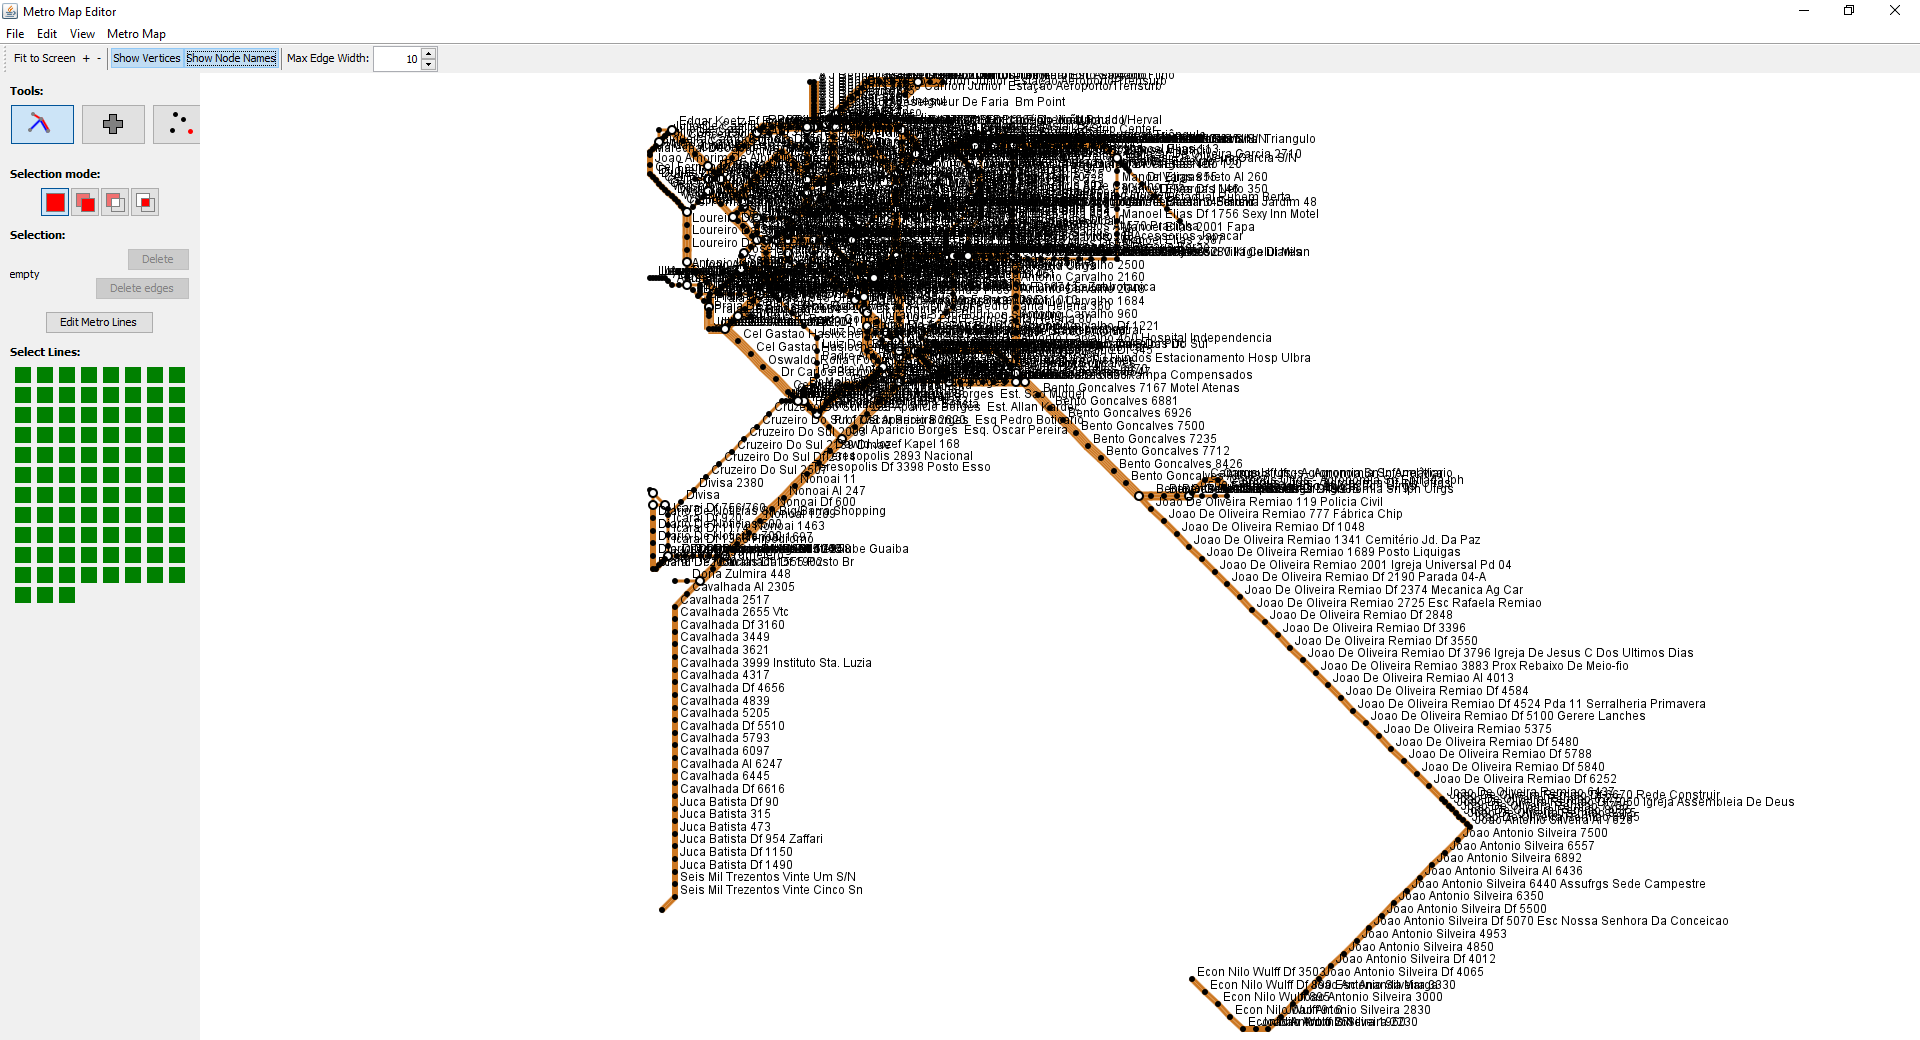
\includegraphics[width=\linewidth, trim=360 2 20 55, clip]{imagens/analiseMapas/nomes.png}
    \caption{Inspeção visual da sobreposição direta de rótulos de paradas.}
    \label{fig:inspecao_nomes}
\end{figure}

Em síntese, o modelo biobjetivo produziu layouts globalmente superiores e mais equilibrados, sobressaindo-se em relação à formulação triobjetiva sobretudo pelo seu custo computacional substancialmente inferior. Essa maior eficiência algorítmica revelou-se um fator determinante na qualidade dos resultados, uma vez que viabilizou a adoção de patamares de \textit{MIP Gap} mais rigorosos sem estourar o limite de tempo estipulado, permitindo ao solver aprofundar a exploração da árvore de busca e encontrar soluções mais refinadas.


\section{Análise Quantitativa}
\label{sec:analise_quantitativa}

\subsection{Grafo Híbrido}
\label{subsec:analise_grafo_hibrido}

A construção do Grafo Híbrido visa solucionar uma limitação intrínseca da estrutura de dados GTFS: enquanto o conjunto de paradas (\texttt{stops.txt} e \texttt{stop\_times.txt}) contém a semântica das viagens e a denominação das estações, ele carece da geometria contínua do traçado das vias; inversamente, os dados de traçado (\texttt{shapes.txt}) fornecem o alinhamento viário geográfico preciso, porém sem a identificação explícita de onde cada parada está situada. O pipeline de pré-processamento proposto integra essas duas fontes por meio da projeção ortogonal (\textit{snapping}) das paradas sobre as arestas do traçado das vias que atendem à rota correspondente, seguida pela supressão de vértices intermediários de traçado sem denominação.

O raio limite de projeção foi fixado em $\delta_{\text{snap}} = 110\,\text{m}$ a partir de calibrações empíricas sobre a base de dados de Porto Alegre. Esse valor correspondeu ao menor limiar de busca capaz de assegurar que \textbf{100\% das paradas físicas cadastradas} fossem devidamente aderidas e ancoradas à malha geométrica de traçados (\textit{shapes}), eliminando completamente a ocorrência de estações órfãs ou desconectadas no grafo.

A aplicação da rotina de validação topológica (detalhada na Seção~\ref{subsec:construcao_grafo_hibrido} e ilustrada na Figura~\ref{fig:fluxo_grafo_hibrido}) sobre a malha integral de ônibus de Porto Alegre produziu os resultados consolidados na Tabela~\ref{tab:estatisticas_grafo_hibrido}. A taxa de retenção global de \textbf{92,89\%} evidencia a consistência da abordagem híbrida com a priorização semântica por compatibilidade de rotas durante o \textit{snapping}. Sem a aplicação desse critério, a taxa de retenção é reduzida para $80{,}26\%$. O modelo com priorização consegue transferir a quase totalidade das informações semânticas e operacionais de paradas para o esqueleto geométrico contínuo das vias. Cabe enfatizar que devido à totalidade das paradas fundidas à malha geográfica, a estatística das paradas faltantes não decorreu por falta das paradas, mas sim por estas paradas terem sido anexadas a arestas incorretas. Esse índice de retenção assegura que a representação simplificada submetida ao solver MIP preserve com alta fidelidade a experiência de viagem e as opções de conexão do sistema de transporte da capital gaúcha.

\begin{table}[H]
    \centering
    \caption{Estatísticas de retenção de paradas na construção do Grafo Híbrido completo de Porto Alegre.}
    \label{tab:estatisticas_grafo_hibrido}
    \begin{tabular}{lrr}
        \toprule
        \textbf{Métrica} & \textbf{Quantidade} & \textbf{Proporção (\%)} \\
        \midrule
        Total de instâncias de paradas nas rotas ($\sum |\mathcal{S}_{\text{stops}}|$) & 16.425 & 100,00\% \\
        Paradas retidas (com priorização semântica) & 15.257 & \textbf{92,89\%} \\
        Paradas retidas (sem priorização) & 13.182 & \textbf{80,26\%} \\
        \bottomrule
    \end{tabular}
\end{table}

\subsection{Calibração dos Limiares de Distância}
\label{subsec:thresholds_distancias}

Na construção do grafo a ser otimizado, a escolha conjunta dos parâmetros $(D_{\text{merge}}, D_{\text{snap}})$ — que definem, respectivamente, a distância máxima para unificar paradas próximas em um único nó e a distância máxima para projetar e inserir uma parada sobre uma aresta adjacente —, empregados na etapa de fusão de paradas descrita na Seção~\ref{subsec:snapping}, desempenha um papel determinante na complexidade topológica do grafo resultante. No contexto da formulação MIP para mapas esquemáticos octolineares, o grau dos vértices ($\deg(v)$) constitui um fator crítico de desempenho.

Dessa forma, a calibração do par $(D_{\text{merge}}, D_{\text{snap}})$ busca maximizar a simplificação de microsegmentos desnecessários e, simultaneamente, \textbf{minimizar o grau máximo do grafo ($\Delta(G)$) e a quantidade de vértices com grau $\deg(v) > 4$}.

Para determinar a configuração ideal, realizou-se uma varredura paramétrica avaliando 36 combinações com $D_{\text{merge}}, D_{\text{snap}} \in \{0, 10, 20, 30, 40, 50\}\,\text{m}$. A Tabela~\ref{tab:grid_thresholds} consolida os resultados obtidos na malha viária de Porto Alegre, indicando em cada célula o grau máximo alcançado ($\Delta$) e, entre parênteses, a contagem total de nós com grau estritamente superior a 4 ($N_{>4}$).

\begin{table}[H]
    \centering
    \caption{Grau máximo ($\Delta$) e quantidade de vértices com grau $> 4$ ($N_{>4}$) para diferentes combinações de limiares de fusão ($D_{\text{merge}}$) e projeção em arestas ($D_{\text{snap}}$).}
    \label{tab:grid_thresholds}
    \begin{tabular}{ccccccc}
        \toprule
        \textbf{$D_{\text{merge}}$ \textbackslash\ $D_{\text{snap}}$} & \textbf{0\,m} & \textbf{10\,m} & \textbf{20\,m} & \textbf{30\,m} & \textbf{40\,m} & \textbf{50\,m} \\
        \midrule
        \textbf{0\,m}  & \cellcolor{yellow!25} 6 (5)  & \cellcolor{yellow!25} 6 (6)  & \cellcolor{yellow!25} 6 (5)  & \cellcolor{green!25} 5 (4)  & \cellcolor{yellow!25} 6 (5)  & \cellcolor{yellow!25} 6 (8)  \\
        \textbf{10\,m} & \cellcolor{yellow!25} 6 (5)  & \cellcolor{yellow!25} 6 (6)  & \cellcolor{yellow!25} 6 (5)  & \cellcolor{green!25} 5 (3)  & \cellcolor{yellow!25} 6 (4)  & \cellcolor{yellow!25} 6 (7)  \\
        \textbf{20\,m} & \cellcolor{yellow!25} 6 (8)  & \cellcolor{yellow!25} 6 (9)  & \cellcolor{yellow!25} 6 (7)  & \cellcolor{yellow!25} 6 (6)  & \cellcolor{green!25} \textbf{5 (3)} & \cellcolor{yellow!25} 6 (8)  \\
        \textbf{30\,m} & \cellcolor{red!25} 7 (8)     & \cellcolor{yellow!25} 6 (9)  & \cellcolor{yellow!25} 6 (7)  & \cellcolor{yellow!25} 6 (5)  & \cellcolor{yellow!25} 6 (3)  & \cellcolor{yellow!25} 6 (4)  \\
        \textbf{40\,m} & \cellcolor{red!25} 7 (16)    & \cellcolor{red!25} 7 (17)    & \cellcolor{yellow!25} 6 (14) & \cellcolor{yellow!25} 6 (11) & \cellcolor{yellow!25} 6 (8)  & \cellcolor{yellow!25} 6 (6)  \\
        \textbf{50\,m} & \cellcolor{yellow!25} 6 (23) & \cellcolor{yellow!25} 6 (24) & \cellcolor{yellow!25} 6 (21) & \cellcolor{yellow!25} 6 (20) & \cellcolor{yellow!25} 6 (16) & \cellcolor{yellow!25} 6 (15) \\
        \bottomrule
    \end{tabular}
    \vspace{0.15cm}
    \par\raggedright\footnotesize\textit{Nota: Células coloridas conforme o grau máximo: verde ($\Delta = 5$), amarelo ($\Delta = 6$) e vermelho ($\Delta = 7$). Formato das células: $\Delta(G) \ (N_{>4})$, com a configuração adotada destacada em negrito.}
\end{table}

Diante do empate entre os pares $(10\,\text{m}, 30\,\text{m})$ e $(20\,\text{m}, 40\,\text{m})$ — ambos atingindo $\Delta(G) = 5$ com apenas 3 nós de grau superior a 4 —, o par $(20\,\text{m}, 40\,\text{m})$ foi selecionado por apresentar limiares maiores, proporcionando maior nível de abstração visual ao mapa e reduzindo de forma mais expressiva a quantidade de nós presentes.

\subsection{Impacto das Etapas de Abstração na Complexidade do Grafo}
\label{subsec:impacto_etapas_abstracao}

A viabilidade computacional da formulação MIP em redes de transporte urbano de grande porte está estritamente condicionada a duas dimensões topológicas: a escala absoluta do grafo (quantificada pelo número de vértices $|V|$ e de arestas $|E|$) e a distribuição dos graus de conectividade dos nós. Em particular, vértices com grau $\deg(v) > 4$ impõem desafios à ordenação circular de arestas e aumentam a árvore de busca (\textit{branch-and-bound}) do solver, enquanto nós com grau superior a 8 violam a capacidade de acomodação de uma grade octolinear.

Para avaliar quantitativamente a eficácia dos métodos de abstração desenvolvidos no módulo de pré-processamento (\texttt{data\_parser.jl}, ilustrado na Figura~\ref{fig:fluxo_arquitetura}), monitorou-se a evolução métrica e estrutural do grafo de Porto Alegre ao longo das quatro principais etapas do pipeline:

\begin{enumerate}
    \item \textbf{Grafo de Paradas Original ($G_{\text{stops}}$):} construído exclusivamente pelas conexões diretas entre paradas consecutivas em cada viagem;
    \item \textbf{Grafo Híbrido ($G_{\text{híbrido}}$):} obtido pela projeção ortogonal das paradas sobre a geometria viária contínua (\texttt{shapes.txt}) com $\delta_{\text{snap}} = 110\,\text{m}$ e subsequente contração de nós de traçado intermediários desprovidos de denominação;
    \item \textbf{Pós Fusão de Paradas:} resultante da aplicação dos limiares calibrados na Seção~\ref{subsec:thresholds_distancias} ($D_{\text{merge}} = 20\,\text{m}$ e $D_{\text{snap}} = 40\,\text{m}$), unificando paradas fisicamente próximas e eliminando microsegmentos redundantes;
    \item \textbf{Pós Remoção de Adjacentes:} aplicação do critério angular $\varphi$ discutido na Seção~\ref{subsec:remocao_paradas_adjacentes}, contraindo vértices intermediários de grau 2 com deflexão fora do intervalo de preservação ($\varphi \notin [80^\circ, 150^\circ]$).
\end{enumerate}

A Tabela~\ref{tab:evolucao_abstracao} sintetiza o impacto de cada uma dessas etapas nas dimensões e na conectividade da rede viária municipal.

\begin{table}[H]
    \centering
    \caption{Evolução da dimensão e da complexidade topológica do grafo de Porto Alegre ao longo das etapas de abstração de dados.}
    \label{tab:evolucao_abstracao}
    \resizebox{\linewidth}{!}{%
    \begin{tabular}{lrrrr}
        \toprule
        \textbf{Etapa do Pipeline} & \textbf{Vértices ($|V|$)} & \textbf{Arestas ($|E|$)} & \textbf{Grau Máx. ($\Delta$)} & \textbf{Nós com $\deg(v) > 4$} \\
        \midrule
        Grafo de Paradas ($G_{\text{stops}}$) & 3.831 & 4.382 & 8 & 61 \\
        Grafo Híbrido ($G_{\text{híbrido}}$)   & 4.858 & 5.368 & 6 & 5 \\
        Pós Fusão de Paradas                  & 4.174 & 4.660 & \textbf{5} & \textbf{3} \\
        Pós Remoção de Adjacentes             & \textbf{1.603} & \textbf{2.071} & \textbf{5} & \textbf{3} \\
        \bottomrule
    \end{tabular}%
    }
\end{table}

Os resultados evidenciam que o pipeline de abstração é determinante para a viabilidade computacional do modelo: a transição para a malha híbrida e a subsequente fusão de paradas eliminaram os vértices de grau crítico ($\Delta = 8 \to 5$, reduzindo de 61 para apenas 3 os nós com $\deg(v) > 4$), enquanto a remoção de paradas colineares adjacentes proporcionou uma contração de $61{,}6\%$ nos vértices (de 4.174 para 1.603) e $55{,}6\%$ nas arestas (de 4.660 para 2.071). Essa simplificação estrutural mitiga o custo combinatório das restrições de ordem circular no solver MIP e viabiliza a convergência da otimização das bacias operacionais de Porto Alegre em tempo hábil, preservando a legibilidade e a coerência topológica da rede.

\subsection{Eficácia da Correção Iterativa Angular}
\label{subsec:analise_correcao_iterativa}

Conforme discutido na Seção~\ref{subsec:correcao_distorcoes}, a imposição direta de restrições de não-cruzamento entre arestas não adjacentes (regras clássicas de complexidade $O(|E|^2)$ propostas por Nöllenburg e Wolff) mostrou-se computacionalmente intratável para redes densas de ônibus como a de Porto Alegre. Para contornar esse obstáculo sem comprometer a integridade visual dos mapas, este trabalho propôs uma abordagem alternativa: o modelo MIP é inicialmente resolvido sem restrições de cruzamento e, em seguida, submetido a um ciclo iterativo que identifica desvios angulares excessivos ($|\Delta\theta| > 100^\circ$) e colapsos de distância sob a norma $L_\infty$ entre pares de nós, reintroduzindo sob demanda apenas restrições direcionais lineares (Equação~\ref{eq:pos_restricao_direcao}).

Para comprovar empiricamente a eficácia dessa proposta e demonstrar que a correção iterativa angular é capaz de restaurar a planaridade e a ordem topológica da rede, realizou-se a quantificação exata dos cruzamentos geométricos entre arestas não-incidentes ao longo das iterações do processo. A Tabela~\ref{tab:evolucao_cruzamentos} compara a contagem de cruzamentos observada na primeira iteração ($i = 1$, antes de qualquer intervenção corretiva) com a solução obtida na última iteração ($i = N$) para cada bacia operacional e formulação avaliada.

\begin{table}[H]
    \centering
    \caption{Comparativo da quantidade de cruzamentos entre a primeira iteração ($i=1$) e a iteração final ($i=N$) do algoritmo de correção iterativa angular.}
    \label{tab:evolucao_cruzamentos}
    \resizebox{\linewidth}{!}{%
    \begin{tabular}{llcccccc}
        \toprule
        \textbf{Bacia Operacional} & \textbf{Formulação} & \textbf{Iter. Final ($N$)} & \textbf{Cruzamentos ($i=1$)} & \textbf{Cruzamentos ($i=N$)} & \textbf{Variação ($\Delta$)} & \textbf{Redução (\%)} & \textbf{Cortes Angulares} \\
        \midrule
        \multirow{2}{*}{Norte / Nordeste (Azul)} 
            & Biobjetiva  & 44 & 85 & \textbf{4} & -81 & \textbf{95,3\%} & 2.435 \\
            & Triobjetiva & 50 & 22 & 12         & -10 & 45,5\%          & 3.638 \\
        \midrule
        \multirow{2}{*}{Sul (Vermelha)} 
            & Biobjetiva  & 11 & 32 & \textbf{4} & -28 & \textbf{87,5\%} & 598 \\
            & Triobjetiva & 34 & 9  & 10         & +1  & -11,1\%         & 462 \\
        \midrule
        \multirow{2}{*}{Leste / Sudeste (Verde)} 
            & Biobjetiva  & 15 & 49 & \textbf{5} & -44 & \textbf{89,8\%} & 1.003 \\
            & Triobjetiva & 14 & 23 & \textbf{5} & -18 & 78,3\%          & 476 \\
        \midrule
        \multirow{2}{*}{Transversais (Laranja)} 
            & Biobjetiva  & 8  & 3  & \textbf{0} & -3  & \textbf{100,0\%}& 28 \\
            & Triobjetiva & 3  & 1  & 1          & 0   & 0,0\%           & 31 \\
        \midrule
        \multirow{2}{*}{\textbf{Total Acumulado}} 
            & \textbf{Biobjetiva}  & --- & \textbf{169} & \textbf{13} & \textbf{-156} & \textbf{92,3\%} & \textbf{4.064} \\
            & \textbf{Triobjetiva} & --- & \textbf{55}  & \textbf{28} & \textbf{-27}  & 49,1\%          & \textbf{4.607} \\
        \bottomrule
    \end{tabular}%
    }
    \vspace{0.15cm}
    \par\raggedright\footnotesize\textit{Nota: A coluna ``Cortes Angulares'' reporta o total acumulado de restrições lineares direcionais adicionadas ao modelo pelo algoritmo até a convergência.}
\end{table}

Os resultados comprovam a eficácia prática e o poder de estabilização topológica do algoritmo de correção iterativa proposto. Na formulação biobjetiva, a realimentação angular eliminou \textbf{92,3\%} dos cruzamentos da malha urbana (reduzindo de 169 para apenas 13), alcançando uma redução de $95{,}3\%$ na Bacia Norte e a planaridade estrita (zero cruzamentos) nas Linhas Transversais, superando amplamente a variante triobjetiva (que estabilizou com 28 cruzamentos). Fundamentalmente, como os cortes inseridos consistem apenas em restrições lineares direcionais e não em restrições combinatórias explícitas de não-cruzamento ($O(|E|^2)$), essa expressiva redução demonstra que os entrelaçamentos acidentais em redes de ônibus decorrem essencialmente de distorções e inversões geográficas macroscópicas. Dessa forma, ao restaurar a coerência angular relativa entre os nós, o algoritmo faz com que grande parte das arestas se desembaracem de maneira natural.

Vale ressalvar, contudo, que a correção angular nem sempre acarreta a redução de cruzamentos em todas as instâncias, como verificado na Bacia Sul sob a formulação triobjetiva, na qual a contagem oscilou ligeiramente de 9 para 10 cruzamentos. Esse comportamento ocorre porque existem cruzamentos geométricos sutis que não são detectados unicamente pela análise angular por envolverem pares de nós cujo desvio $|\Delta\theta|$ permaneça dentro da faixa de tolerância de $100^\circ$. Todavia, mesmo com a presença dessas exceções pontuais, o método comprovou ser amplamente eficaz no balanço global, eliminando a grande maioria dos conflitos topológicos sem incorrer no custo computacional proibitivo das formulações de não-cruzamento.

\subsection{Desempenho Computacional e Convergência das Otimizações MIP}
\label{subsec:desempenho_computacional_mip}

A resolução exata dos modelos matemáticos foi conduzida no cluster computacional Phoenix sobre os quatro recortes operacionais do sistema de transporte de Porto Alegre. Para cada subconjunto viário, foram executadas tanto a formulação biobjetiva quanto a triobjetiva, acopladas ao loop iterativo de detecção e realimentação de restrições angulares e de sobreposição espacial não-adjacente. A Tabela~\ref{tab:desempenho_mip} consolida as métricas computacionais extraídas dos registros de execução do solver CPLEX 22.1.1.0 e da análise topológica dos grafos resultantes, contemplando o esforço algorítmico do \textit{branch-and-bound}, o tempo de processamento total acumulado, a contagem de cruzamentos entre arestas e a qualidade geométrica final atestada pelo diagnóstico pós-otimização.

Para cada solução obtida, verificou-se a quantidade de cruzamentos gerados entre arestas não-incidentes, fenômeno que constitui uma degradação topológica da rede. Adicionalmente, quantificou-se a presença de vértices posicionados sobre arestas não-adjacentes, uma vez que tais sobreposições não apenas geram interpretações topológicas incorretas no mapa final, como também podem mascarar cruzamentos geométricos caso um vértice colapse exatamente sobre o traçado de uma aresta à qual não pertence.

\begin{table}[H]
    \centering
    \caption{Desempenho computacional e métricas de convergência do solver CPLEX para as formulações biobjetiva e triobjetiva por bacia operacional.}
    \label{tab:desempenho_mip}
    \resizebox{\linewidth}{!}{%
    \begin{tabular}{llccrrrcc}
        \toprule
        \textbf{Bacia Operacional} & \textbf{Formulação} & \textbf{$|V|$} & \textbf{$|E|$} & \textbf{Iterações} & \textbf{Restr. Angulares} & \textbf{Tempo Total (s)} & \textbf{Cruzamentos} & \textbf{Sobreposições Finais} \\
        \midrule
        \multirow{2}{*}{Norte / Nordeste (Azul)} 
            & Biobjetiva  & 588 & 760 & 44 & 2.435 & 33.393{,}9 & \textbf{4} & \textbf{1} \\
            & Triobjetiva & 588 & 760 & 50 & 3.638 & 18.840{,}7 & 12 & 17 \\
        \midrule
        \multirow{2}{*}{Sul (Vermelha)} 
            & Biobjetiva  & 480 & 578 & 11 & 598   & 6.832{,}6  & \textbf{4} & \textbf{5} \\
            & Triobjetiva & 480 & 578 & 34 & 462   & 31.496{,}1 & 10 & 14 \\
        \midrule
        \multirow{2}{*}{Leste / Sudeste (Verde)} 
            & Biobjetiva  & 522 & 635 & 15 & 1.003 & 6.493{,}5  & \textbf{5} & \textbf{4} \\
            & Triobjetiva & 522 & 635 & 14 & 476   & 10.490{,}5 & \textbf{5} & 11 \\
        \midrule
        \multirow{2}{*}{Transversais (Laranja)} 
            & Biobjetiva  & 260 & 319 & 8  & 28    & \textbf{185{,}5}   & \textbf{0} & 3 \\
            & Triobjetiva & 260 & 319 & 3  & 31    & 415{,}0    & 1 & 3 \\
        \bottomrule
    \end{tabular}%
    }
\end{table}

A análise comparativa dos dados empíricos evidencia as causas fundamentais das diferenças de comportamento observadas entre as abordagens:

\begin{enumerate}
    \item \textbf{Complexidade Estrutural do Modelo:} A formulação triobjetiva otimiza as arestas de forma a penalizar a extensão de cada segmento na grade discreta. Essa flexibilização amplia consideravelmente o espaço contínuo relaxado da formulação e impõe um esforço substancialmente maior durante a geração de planos de \textit{branch-and-bound} da árvore no solver;
    \item \textbf{Tempo Computacional e Impacto da Tolerância de Otimalidade (\textit{MIP Gap}):} Na Bacia Sul (Vermelha), enquanto a variante biobjetiva convergiu plenamente em 11 iterações demandando um total de 6.832{,}6 segundos (1,9 horas), a variante triobjetiva exigiu 34 iterações e acumulou 31.496{,}1 segundos (8,7 horas). Mesmo nas Linhas Transversais (Laranja), cuja topologia mais enxuta possui 260 vértices, o tempo despendido pela versão triobjetiva (415{,}0\,s) foi mais do que o dobro do registrado pela biobjetiva (185{,}5\,s). Essa disparidade temporal torna-se ainda mais expressiva quando se considera que a formulação triobjetiva foi configurada um \textit{MIP Gap} consideravelmente mais permissivos (conforme Tabela~\ref{tab:mipgap_bacias}). Isso evidencia que, caso a variante triobjetiva fosse submetida aos mesmos níveis rigorosos de convergência da biobjetiva, o tempo de resolução extrapolaria os limites operacionais estipulados, comprovando a ineficiência computacional intrínseca da penalização suave de comprimentos;
    \item \textbf{Dinâmica do Mecanismo de Realimentação Angular ($|\Delta\theta|$):} O processo iterativo de corte angular comprovou ser altamente eficiente para estabilizar a coerência geográfica global. Em redes densas como a Bacia Norte e a Bacia Leste, o algoritmo identificou e corrigiu milhares de distorções pontuais (2.435 restrições adicionadas na Bacia Azul biobjetiva e 1.003 na Bacia Verde biobjetiva), garantindo que os mapas finais ficassem livres de inversões direcionais drásticas;
    \item \textbf{Ocorrência de Cruzamentos entre Arestas:} A análise topológica dos arquivos \textit{GraphML} finais demonstrou que a formulação biobjetiva foi substancialmente mais eficaz em minimizar cruzamentos acidentais entre arestas não-incidentes. Na Bacia Norte, o modelo biobjetivo registrou apenas 4 cruzamentos contra 12 na triobjetiva; na Bacia Sul, foram 4 cruzamentos na biobjetiva contra 10 na triobjetiva; e no subsistema das Linhas Transversais, a solução biobjetiva alcançou uma representação estritamente planar (0 cruzamentos na malha otimizada), contra 1 na triobjetiva. Esse comportamento decorre da rigidez dimensional imposta pelo modelo biobjetivo, que restringe deslocamentos excessivos de vértices;
    \item \textbf{Incidência de Sobreposições Topológicas Finais:} A última coluna da Tabela~\ref{tab:desempenho_mip} reporta a contagem de nós localizados sobre arestas não-adjacentes no diagnóstico pós-otimização. Constata-se que a formulação biobjetiva apresentou uma contenção expressivamente superior de sobreposições: na Bacia Norte, registrou-se apenas 1 nó sobreposto na biobjetiva contra 17 na triobjetiva; na Bacia Leste, 4 contra 11; e na Bacia Sul, 5 contra 14. 
\end{enumerate}

Esses indicadores quantitativos justificam e confirmam as conclusões estéticas obtidas na Seção~\ref{sec:analise_qualitativa}: o modelo biobjetivo não apenas demonstrou ser computacionalmente mais ágil e tratável para instâncias urbanas de grande escala, como também produziu mapas com sensivelmente menos cruzamentos de linhas, menor taxa de colapso de nós e maior desobstrução visual, estabelecendo-se como a formulação mais recomendável para a esquematização da malha viária avaliada.

\chapter{Conclusão}
\label{cap:conclusao}

Este trabalho investigou a aplicação de técnicas de Programação Inteira Mista (MIP) para a geração automatizada de mapas esquemáticos octilineares do sistema de transporte público por ônibus de Porto Alegre, partindo exclusivamente de dados abertos no padrão GTFS. Ao transpor o problema clássico de esquematização cartográfica — tradicionalmente restrito a redes de metrô e modais sobre trilhos com topologias compactas e regulares — para a complexa malha viária rodoviária urbana de uma metrópole brasileira, esta pesquisa delimitou tanto as potencialidades estéticas do paradigma exato quanto os limites práticos de sua escalabilidade computacional.

\section{Síntese do Trabalho}
\label{sec:sintese_trabalho}

Para viabilizar a otimização matemática sobre uma base de dados ruidosa e fragmentada, foi desenvolvido um pipeline de pré-processamento que integrou as paradas físicas (\texttt{stops.txt}) à geometria contínua das vias (\texttt{shapes.txt}). Esse procedimento resultou na construção do Grafo Híbrido, cuja técnica de \textit{snapping} com priorização semântica por rota alcançou uma taxa global de retenção de 92,89\% das paradas cadastradas. Subsequentemente, a calibração de limiares de fusão ($D_{\text{merge}} = 20\,\text{m}$, $D_{\text{snap}} = 40\,\text{m}$) e a contração angular de vértices adjacentes de grau 2 reduziram a escala da rede metropolitana em mais de 58\% (de 3.831 para 1.603 vértices), reduzindo a quantidade de nós de maior grau ($\Delta(G) > 4$) que dificultavam a solução de restrições circulares.

A experimentação comparou duas formulações matemáticas acopladas a um loop iterativo de cortes geométricos: a formulação biobjetiva (baseada em Oke e Siddiqui, com cota rígida de comprimento) e a triobjetiva (utilizando todas as adaptações de Oke, com exceção da transformação da penalidade de tamanho de aresta para uma restrição). As otimizações foram executadas no ambiente de alto desempenho do cluster Phoenix sobre os quatro principais recortes operacionais da cidade (Bacias Norte, Sul, Leste e Linhas Transversais).

Os resultados quantitativos e visuais comprovaram que a esquematização automatizada via MIP é factível e produz diagramas de alta qualidade geométrica para bacias urbanas individuais. Em todas as instâncias avaliadas, a formulação biobjetiva sobressaiu-se amplamente: além de exigir um custo computacional sensivelmente inferior (reduzindo tempos de execução de 8,7 horas para menos de 2 horas na Bacia Sul), a sua rigidez dimensional restringiu o estiramento desordenado de arestas, resultando em até três vezes menos cruzamentos acidentais e numa contenção substancialmente mais eficaz de sobreposições nodais.

Não obstante o sucesso alcançado nas bacias individuais, a investigação revelou empiricamente a existência de uma barreira intransponível de escalabilidade para os modelos de otimização linear exata. Mesmo dispondo de infraestrutura computacional de grande porte (44 \textit{threads} e 110\,GB de memória dedicados à árvore de busca) e empregando o modelo relaxado de Oke e Siddiqui, a malha viária integral de Porto Alegre — congregando mais de 1.600 vértices mesmo após profunda simplificação topológica — revelou-se insolúvel dentro dos horizontes temporais práticos. Conclui-se, portanto, que redes completas de transporte rodoviário urbano de grande porte situam-se além da fronteira de tratabilidade direta dos solucionadores MIP contemporâneos, demandando abordagens modulares ou particionadas para sua viabilização.

\section{Contribuições}
\label{sec:contribuicoes}

As principais contribuições técnico-científicas desenvolvidas ao longo deste trabalho compreendem:

\begin{enumerate}
    \item \textbf{Metodologia de Fusão Topológica para Dados GTFS:} Formulação de um fluxo algorítmico automatizado para harmonização entre traçados geométricos contínuos e sequências pontuais de paradas, garantindo que 100\% das estações físicas fossem ancoradas à malha sem a geração de vértices desconectados;
    \item \textbf{Estratégia de Redução de Complexidade Estrutural:} Estabelecimento de regras heurísticas de contração baseadas no ângulo $\varphi$ e varredura paramétrica de distâncias que diminuíram drasticamente o grau máximo da rede ($\Delta(G)$ reduzido para 5), tornando tratáveis as restrições lineares de ordenamento angular ao redor dos nós;
    \item \textbf{Mecanismo Iterativo de Estabilização Topológica:} Proposição e implementação de um ciclo de realimentação que identifica dinamicamente violações de orientação geográfica ($|\Delta\theta| > 100^\circ$) e colapsos em distância $L_\infty$, reinserindo cortes lineares sem a sobrecarga computacional de proibir exaustivamente todos os cruzamentos da malha viária;
    \item \textbf{Estudo Comparativo Inédito em Cenário Real:} Avaliação empírica detalhada entre abordagens biobjetivas e triobjetivas com enfoque no transporte público por ônibus em Porto Alegre, RS, fornecendo parâmetros objetivos de \textit{MIP Gap}, tempos de resolução, contagem geométrica de cruzamentos e índices de sobreposição.
\end{enumerate}

\section{Trabalhos Futuros}
\label{sec:trabalhos_futuros}

A partir dos desafios e das oportunidades identificados ao longo do projeto, sugerem-se as seguintes direções para investigações futuras:

\begin{enumerate}
    \item \textbf{Aperfeiçoamento da Construção do Grafo Híbrido:} Embora o pipeline proposto tenha atingido uma taxa de retenção expressiva de 92,89\% das paradas cadastradas, a representação ainda não alcançou a exatidão absoluta (100\%). Uma frente de pesquisa essencial consiste no desenvolvimento de técnicas mais robustas de fusão e desambiguação espacial, visando eliminar completamente as perdas de paradas vinculadas a arestas incorretas e obter um grafo perfeitamente aderente à realidade operacional das linhas de Porto Alegre;
    \item \textbf{Desenvolvimento de Interface Gráfica (GUI) e Estudos de UI/UX:} Conforme evidenciado na Seção~\ref{sec:analise_qualitativa} (Figura~\ref{fig:inspecao_nomes}), a visualização clássica adaptada do visualizador Java/JUNG não oferece recursos adequados para a inspeção de redes complexas, omitindo a identificação textual clara de itinerários e estações. Torna-se imperativo o desenvolvimento de uma interface interativa moderna com suporte a camadas, filtros operacionais por bacia e níveis dinâmicos de detalhe (\textit{zoom levels}), fundamentada em princípios de ergonomia visual e experiência do usuário (UI/UX);
    \item \textbf{Algoritmos Dedicados de Posicionamento de Rótulos:} A simples sobreposição direta dos nomes das paradas compromete a legibilidade de grafos viários densos. Propõe-se integrar uma etapa pós-MIP baseada em técnicas dedicadas de posicionamento cartográfico de rótulos (como as propostas por Nöllenburg e Wolff para metrô), otimizando a rotação e a alocação de caixas textuais ao longo dos corredores desobstruídos;
    \item \textbf{Ordenação Fina de Linhas nos Segmentos:} Aplicar sobre a malha esquematizada as diretrizes metodológicas de Sadahiro et al. \cite{Sadahiro2016} e Brosi e Bast \cite{brosi2023large}, determinando a ordem relativa das rotas paralelas em cada segmento viário a fim de minimizar lacunas vazias (\textit{gaps}) e deslocamentos laterais espúrios (\textit{shifts}).
    \item \textbf{Aperfeiçoamento na Calibração de Parâmetros e Limiares Heurísticos:} Embora limiares essenciais tenham sido calibrados experimentalmente, como a fusão e projeção de paradas $(D_{\text{merge}}, D_{\text{snap}})$ investigadas na Seção~\ref{subsec:thresholds_distancias} (Tabela~\ref{tab:grid_thresholds}), diversos outros parâmetros foram definidos heuristicamente. Recomenda-se conduzir análises ou calibração automática de hiperparâmetros sobre fatores determinantes do pipeline, tais como os limites angulares $[\varphi_{\min}, \varphi_{\max}]$ para remoção de paradas adjacentes (Seção~\ref{subsec:remocao_paradas_adjacentes}), o limiar de tolerância ao desvio $|\Delta\theta|$ no mecanismo corretivo iterativo (Seção~\ref{subsec:correcao_distorcoes}), as dimensões da grade discreta ($\text{GRID\_WIDTH}$ e $\text{GRID\_HEIGHT}$) com seus impactos no Big-$M$ e a ponderação dos pesos da função objetivo (Seção~\ref{subsec:parametros_solver}).

\end{enumerate}

%==============================================================================
% Back matter
%==============================================================================

% Appendices start with \appendix (optional \annexname for annexes)
% \appendix

% \chapter{Exemplo de Apêndice}

% Apêndices contêm material elaborado pelo próprio autor.

% \annex

% \chapter{Exemplo de Anexo}

% Anexos contêm material de terceiros reproduzido para documentação.

%------------------------------------------------------------------------------
% References (ABNT author-date style)
%------------------------------------------------------------------------------
\bibliographystyle{abntex2-alf}
\bibliography{tcc-gustavo}

\end{document}
